\documentclass{book}
\usepackage{graphicx} % Required for inserting images

\graphicspath{ {./images/} }
\usepackage{geometry}
\usepackage{hyperref}
\usepackage{amsmath}
\usepackage{amsfonts}
\newgeometry{
left=   1 in,
bottom= 1.5 in,
right=  1 in,
top=    1 in
}

\title{Data Mining Notes}
\author{Riccardo Cappi}
\date{June 2024}

\begin{document}

\maketitle

\section{Disclaimer}
These are just my notes that I used to prepare for the exam. So, probably, there will be both spelling and conceptual errors. Feel free to contact me at riccardo.cappi@studenti.unipd.it if you find any errors. This is the github repo where you can find the latex files of the notes: \url{https://github.com/riccardocappi/Computer-Science-notes}

\tableofcontents

\chapter{Lec 03 - PCA}

\section{Unsupervised Learning}
Most of this course focuses on \textbf{supervised learning} methods such as regression and classification. In that setting we observe both a set of features $X_1, X_2, . . . , X_p$ for each object, as well as a response or
outcome variable $Y$. The goal is then to predict $Y$ using $X_1, X_2, . . . , X_p$.\\\\
Here we instead focus on \textbf{unsupervised learning}, where we observe only the features $X_1, X_2, . . . , X_p$. We are not interested in prediction, because we do not have an associated response variable $Y$. The goal is to discover interesting things about the measurements: is there an informative way to visualize the data? Can we discover subgroups among the variables or among the observations?

\section{Recall of mean, variance, covariance}
Recall of the formulas for mean, variance and covariance:
\begin{itemize}
    \item \textbf{Mean:} $\overline{X} = \frac{1}{n}\sum_{i=1}^n x_i$

    \item \textbf{Variance:} $Var(X) = \frac{1}{n}\sum_{i=1}^n (x_i - \overline{X})^2$

    \item \textbf{Covariance:} $Cov(X,Y) = \frac{1}{n}\sum_{i=1}^n (x_i - \overline{X})(y_i - \overline{Y})$
\end{itemize}

\section{Principal Components Analysis (PCA)}
PCA produces a low-dimensional representation of a dataset. It finds a sequence of linear combinations of the variables that have maximal variance, and are mutually uncorrelated.
\\\\
PCA is an unsupervised approach, since it involves only a set of features $X_1, X_2,...,X_p$, and no associated response $Y$. Apart from producing derived variables for use in supervised learning problems, PCA also serves as a tool for data visualization.

\subsection{What Are Principal Components?}
Suppose that we wish to visualize $n$ observations with measurements on a
set of $p$ features, $X_1, X_2,...,X_p$, as part of an exploratory data analysis. We would like to find a low-dimensional representation of the data that captures as much of the information as possible. For instance, if we can obtain a two-dimensional representation of the data that captures most of the information, then we can plot the observations in this low-dimensional space.\\\\
PCA provides a tool to do just this. It finds a low-dimensional representation of a data set that contains as much as possible of the variation. The idea is that each of the $n$ observations lives in $p$-dimensional space, but not all of these dimensions are equally interesting. PCA seeks a small number of dimensions that are as interesting as possible, where the concept of interesting is measured by the amount that the observations vary along each dimension.  Each of the dimensions found by PCA is a linear combination of the $p$ features. We now explain the manner in which these dimensions, or principal components, are found.\\\\
The \textit{first principal component} of a set of features $X_1, X_2,...,X_p$ is the normalized linear combination of the features
\[Z_1 = \phi_{11}X_1 + \phi_{21}X_2 + ... +\phi_{p1}X_p\]
that has the largest variance. By normalized, we mean that $\sum_{j=1}^p \phi_{j1}^2 = 1$. We refer to the elements $\phi_{11},...,\phi_{p1}$ as the loadings of the first principal component; together, the loadings make up the principal component loading vector $\phi_1$. We constrain the loadings so that their sum of squares is equal to one, since otherwise setting these elements to be arbitrarily large in absolute value could result in an arbitrarily large variance.\\\\
Given a $n \times p$ data set $\textbf{X}$, how do we compute the first principal component? Since we are only interested in variance, we assume that each of the variables in $\textbf{X}$ has been centered to have mean zero (that is, the column means of $\textbf{X}$ are zero) \footnote{We can do this by subtracting the mean of each column from the values of that column.}. We then look for the linear combination of the sample feature values of the form:
\begin{equation}
    z_{i1} = \phi_{11}x_{i1} + \phi_{21}x_{i2} + ... +\phi_{p1}x_{ip}
    \label{z}
\end{equation}
that has \textbf{largest sample variance}, subject to the constraint that $\sum_{j=1}^p \phi_{j1}^2 = 1$. In other words, the first principal component loading vector solves the optimization problem:
\begin{equation}
    \text{maximize}_{\phi_{11}, ..., \phi_{p1}}\left\{\frac{1}{n}\sum_{i=1}^n\left(\sum_{j=1}^p \phi_{j1}x_{ij}\right)^2\right\} \quad \text{subject to } \sum_{j=1}^p \phi_{j1}^2 = 1
    \label{first comp}
\end{equation}
From \ref{z}, we can write the objective in \ref{first comp} as:
\[\frac{1}{n}\sum_{i=1}^n z_{i1}^2\]
Note that in \ref{first comp} the variance is computed without subtracting the mean because, since $\frac{1}{n}\sum_{i=1}^n x_{i,j} = 0$,  the average of the $z_{11},...,z_{n1}$ will be zero as well. Hence the objective that we are maximizing in \ref{first comp}  is just the sample variance of the $n$ values of $z_{i1}$. We refer to $z_{11},...,z_{n1}$ as the \textit{scores} of the first principal component. Problem \ref{first comp} can be solved via an eigendecomposition, a standard technique in linear algebra.\\\\
There is a nice geometric interpretation for the first principal component. The loading vector $\phi_1$ with elements $\phi_{11}, \phi_{21},...,\phi_{p1}$ defines a direction in feature space along which the data vary the most. If we project the $n$ data points $x_1,...,x_n$ onto this direction, the projected values are the principal component scores $z_{11},...,z_{n1}$ themselves. 

\subsection{Example}
From the figure below we can see that The green solid line represents the first principal component direction of the data. We can see by eye that this is the direction along which there is the greatest variability in the data. That is, if we projected the 100 observations onto this line, then the resulting projected observations would have the largest possible variance.
\begin{center}
    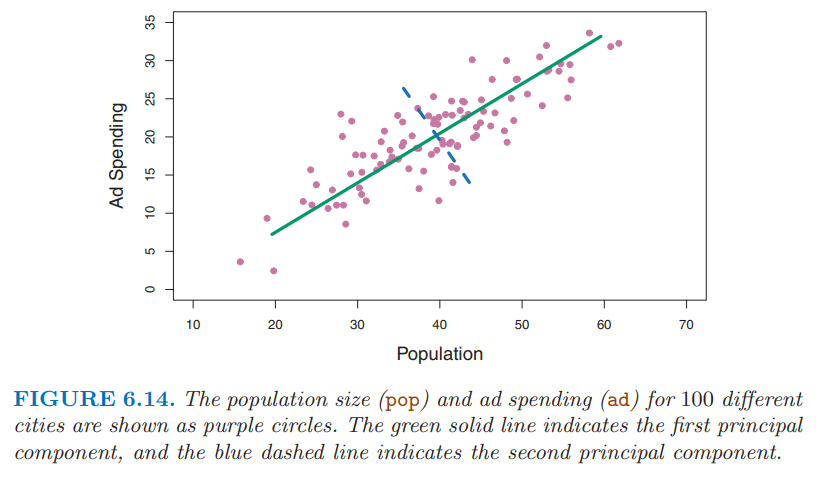
\includegraphics[scale=0.8]{images/first princ comp.png}
\end{center}
Projecting a point onto a line simply involves finding the location on the line which is closest to the point. The first principal component in the figure is given by the formula:
\begin{equation}
    Z_1 = 0.839 \times (pop - \overline{pop}) + 0.544 \times (ad - \overline{ad})
    \label{example}
\end{equation}
Here $\phi_{11} = 0.839$ and $\phi_{21} = 0.544$ are the principal component loadings, which define the direction referred to above. In \ref{example}, $\overline{pop}$ indicates the mean of all $pop$ values in this data set, and $\overline{ad}$ indicates the mean of all advertising spending. The idea is that out of every possible linear combination of $pop$ and $ad$ such that $\phi_{11}^2 + \phi_{21}^2 = 1$, this particular linear combination
yields the highest variance: i.e. this is the linear combination for which $Var(\phi_{11} \times (pop - \overline{pop}) + \phi_{21} \times (ad - \overline{ad}))$ is maximized.

\subsection{Further principal components}
After the first principal component $Z_1$ of the features has been determined, we can find the second principal component $Z_2$. The second principal component is the linear combination of $X_1,...,X_p$ that has maximal variance out of all linear combinations that are \textit{uncorrelated} with $Z_1$. The second principal component scores $z_{12}, z_{22},...,z_{n2}$ take the form
\[z_{i2} = \phi_{12} x_{i1} + \phi_{22}x_{i2} + ... + \phi_{p2} x_{ip}\]
where $\phi_2$ is the second principal component loading vector.  It turns out that constraining $Z_2$ to be uncorrelated with $Z_1$ is equivalent to constraining the direction $\phi_2$ to be orthogonal (perpendicular) to the direction $\phi_1$, and so on.\\\\
Once we have computed the principal components, we can plot them
against each other in order to produce low-dimensional views of the data. For instance, we can plot the score vector $Z_1$ against $Z_2$, $Z_1$ against $Z_3$,
$Z_2$ against $Z_3$, and so forth.\\\\
We illustrate the use of PCA on the \textbf{USArrests} data set. For each of the
50 states in the United States, the data set contains the number of arrests
per 100,000 residents for each of three crimes: \textbf{Assault}, \textbf{Murder}, and \textbf{Rape}. We also record \textbf{UrbanPop} (the percent of the population in each state living in urban areas). The principal component score vectors have length $n = 50$, and the principal component loading vectors have length $p = 4$. PCA was performed after standardizing each variable to have mean zero and standard deviation one.
\begin{center}
    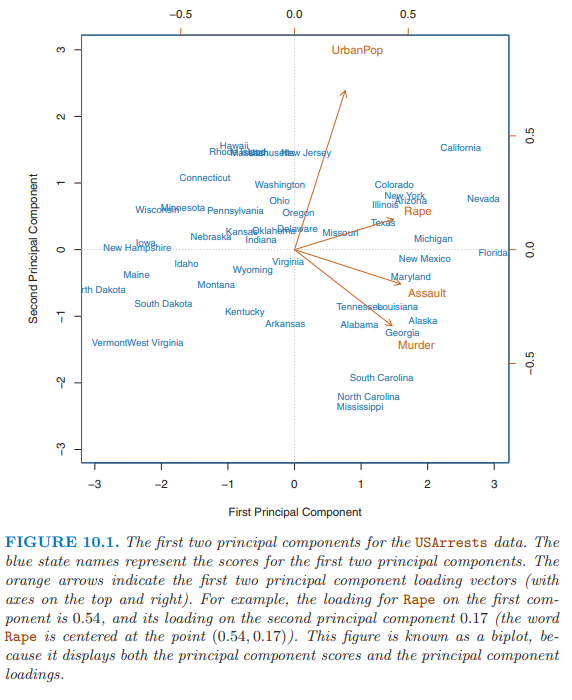
\includegraphics[]{images/biplot.png}
\end{center}
The figure above plots the first two principal components of these data. The figure represents both the principal component scores and the loading vectors in a single biplot display. The loadings are also given in the table below: 
\begin{center}
    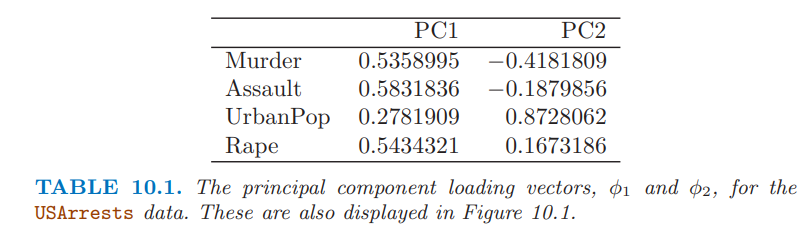
\includegraphics[scale=0.6]{images/table.png}
\end{center}
From the figure we see that the first loading vector places approximately
equal weight on \textbf{Assault}, \textbf{Murder}, and \textbf{Rape}, with much less weight on \textbf{UrbanPop}. Hence this component roughly corresponds to a measure of overall rates of serious crimes. The second loading vector places most of its weight
on \textbf{UrbanPop} and much less weight on the other three features. Hence, this
component roughly corresponds to the level of urbanization of the state. Overall, we see that the crime-related variables (\textbf{Murder}, \textbf{Assault}, and \textbf{Rape}) are located close to each other, and that the \textbf{UrbanPop} variable is far from the other three. This indicates that the crime-related variables are correlated with each other—states with high murder rates tend to have high
assault and rape rates—and that the \textbf{UrbanPop} variable is less correlated with the other three.\\\\
We can examine differences between the states via the two principal component score vectors shown in the figure. Our discussion of the loading vectors suggests that states with large positive scores on the first component, such as California, Nevada and Florida, have high crime rates, while states like North Dakota, with negative scores on the first component, have low crime rates. California also has a high score on the second component, indicating a high level of urbanization, while the opposite is true for states like Mississippi. States close to zero on both components, such as Indiana, have approximately average levels of both crime and urbanization.

\section{Another Interpretation of Principal Components}
The first two principal component loading vectors in a simulated three-dimensional data set are shown in the left-hand panel of the Figure below.
\begin{center}
    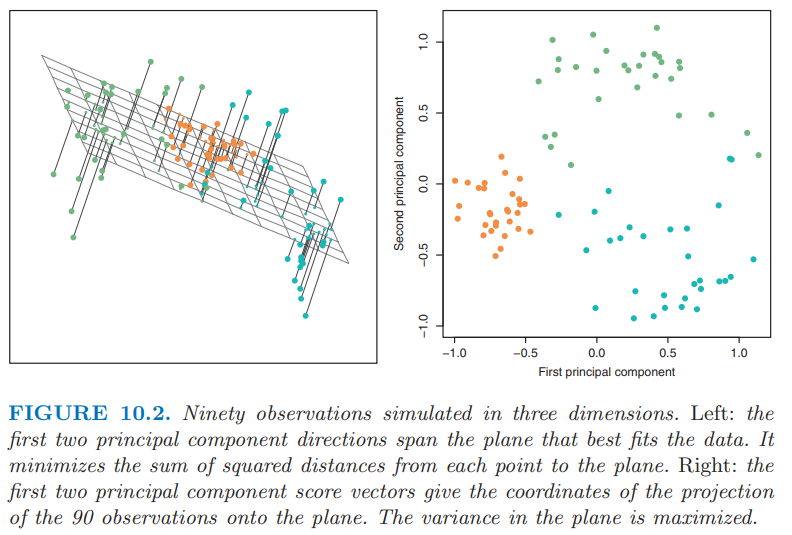
\includegraphics[scale=0.8]{images/3d pca.png}
\end{center}
Principal components provide low-dimensional linear surfaces that are closest to the observations. We expand upon that interpretation here. The first principal component loading vector has a very special property: it is the line in $p$-dimensional space that is closest to the n observations (using average squared Euclidean distance as a measure of closeness). The appeal of this interpretation is clear: we seek a single dimension of the data that lies as close as possible to all of the data points, since such a line will likely provide a good summary of the data.\\\\
The notion of principal components as the dimensions that are closest to the n observations extends beyond just the first principal component.  For instance, the first two principal components of a data set span the plane that is closest to the n observations, in terms of average squared Euclidean distance.

\section{Scaling the Variables}
We have already mentioned that before PCA is performed, the variables should be centered to have mean zero. Furthermore, the results obtained when we perform PCA will also depend on whether the variables have been individually scaled (each multiplied by a different constant).
\begin{center}
    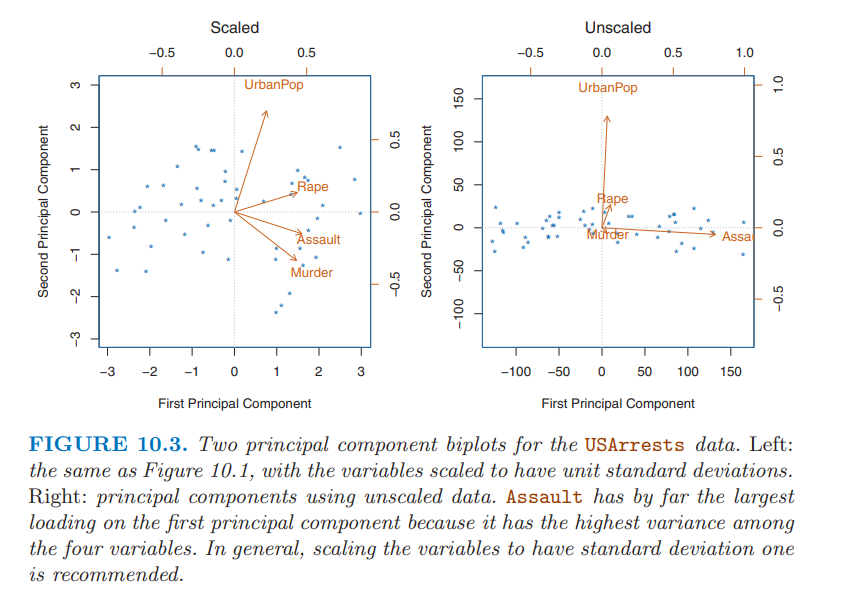
\includegraphics[scale=0.8]{images/scaled pca.png}
\end{center}
From the figure above, we see that scaling does indeed have a substantial effect on the results obtained. In these data, the variables are measured in different units; \textbf{Murder}, \textbf{Rape}, and \textbf{Assault} are reported as the number of occurrences per 100, 000 people, and \textbf{UrbanPop} is the percentage of the state’s population that lives in an urban area. These four variables have variance 18.97, 87.73, 6945.16, and 209.5, respectively. Consequently, if we perform PCA on the unscaled variables, then the first principal component loading vector will have a very large loading for \textbf{Assault}, since that variable has by far the highest variance.
\\\\
Because it is undesirable for the principal components obtained to depend on an arbitrary choice of scaling, we typically scale each variable to have standard deviation one before we perform PCA. In certain settings, however, the variables may be measured in the same units. In this case, we might not wish to scale the variables to have standard deviation one before performing PCA.

\section{The Proportion of Variance Explained}
In Figure 10.2, we performed PCA on a three-dimensional data set (lefthand panel) and projected the data onto the first two principal component loading vectors in order to obtain a two-dimensional view of the data  (i.e. the principal component score vectors; right-hand panel). We see that this two-dimensional representation of the three-dimensional data does successfully capture the major pattern in the data.\\\\
We can now ask a natural question: how much of the information in a given data set is lost by projecting the observations onto the first few principal components? That is, how much of the variance in the data is not contained in the first few principal components? More generally, we are interested in knowing the \textbf{proportion of variance explained} (PVE) by each principal component.\\\\
The total variance present in a data set (assuming that the variables have been centered to have mean zero) is defined as:
\[\sum_{j=1}^p Var(X_j) = \sum_{j=1}^p \frac{1}{n} \sum_{i=1}^n x_{ij}^2\]
and the variance explained by the $m$-th principal component is
\[\frac{1}{n}\sum_{i=1}^n z_{im}^2\]
Therefore, the PVE of the $m$-th principal component is given by:
\[\frac{\sum_{i=1}^n z_{im}^2}{\sum_{j=1}^p\sum_{i=1}^n x_{ij}^2}\]
In total, there are $min(n - 1, p)$ principal components, and their PVEs sum to one.

\section{Deciding How Many Principal Components to Use}
If we use principal components as a summary of our data, how many components are sufficient?  Unfortunately, there is no single (or simple!) answer to this question. We typically decide on the number of principal components required to visualize the data by examining a scree plot, such as the one shown in the left-hand panel of Figure 10.4.
\begin{center}
    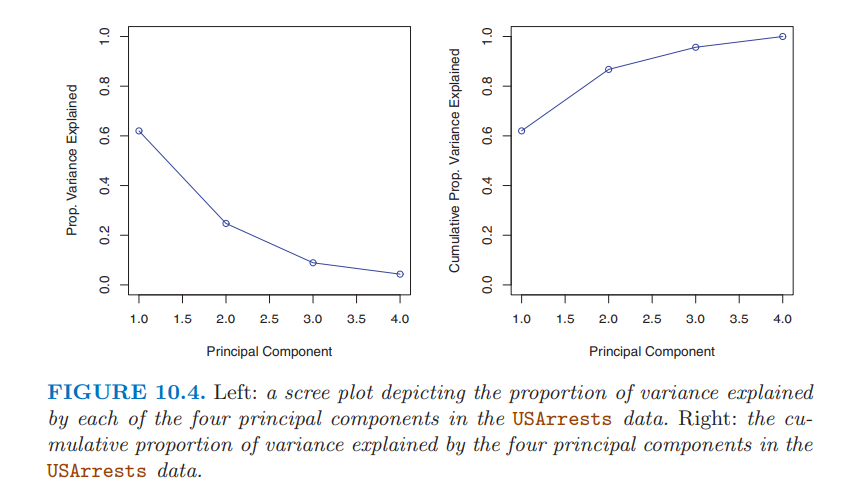
\includegraphics[scale=0.8]{images/scree plot.png}
\end{center}

\chapter{Lec 04 - 05 - Statistical Learning}

\maketitle

\section{What Is Statistical Learning?}
In order to motivate our study of statistical learning, we begin with a simple example. Suppose that we are statistical consultants hired by a client to provide advice on how to improve sales of a particular product. The Advertising data set consists of the sales of that product in 200 different markets, along with advertising budgets for the product in each of those markets for three different media: TV, radio, and newspaper.\\\\
In this setting, the advertising budgets are \textit{input} variables while sales is an \textit{output} variable. The input variables are typically denoted using the symbol $X$, with a subscript to distinguish them. So $X_1$ might be the TV budget, $X_2$ the radio budget, and $X_3$ the newspaper budget. The inputs go by different names, such as \textit{predictors}, \textit{independent variables}, \textit{features}, while the output variable—in this case, sales—is often called the \textit{response}.
\begin{center}
    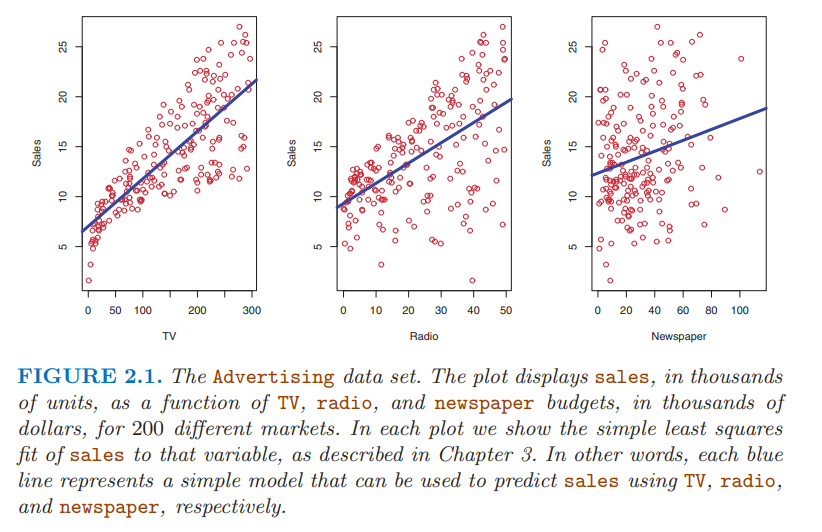
\includegraphics[scale=0.8]{images/tv adv.png}
\end{center}
More generally, suppose that we observe a quantitative response $Y$ and $p$
different predictors, $X_1, X_2,...,X_p$. We assume that there is some
relationship between $Y$ and $X = (X_1, X_2,...,X_p)$, which can be written
in the very general form
\[Y = f(X) + \epsilon\]
Here $f$ is some fixed but \textbf{unknown function} of $X_1,...,X_p$, and $\epsilon$ is a random error term, which is independent of $X$ and has mean zero \footnote{ $\epsilon$ captures measurement errors and other discrepancies}.  In this formulation, $f$ represents the systematic information that $X$ provides about $Y$. In essence, statistical learning refers to a set of approaches for \textbf{estimating}
$f$. 


\section{Prediction}
With a good estimate for $f$ we can make predictions of $Y$ at new points $X = x$. We can predict $Y$ using
\[\hat{Y} = \hat{f}(X)\]
where $\hat{f}$ represents our estimate for $f$, and $\hat{Y}$ represents the resulting prediction for $Y$. The accuracy of $\hat{Y}$ as a prediction for $Y$ depends on two quantities, which we will call the \textit{reducible error} and the \textit{irreducible error}. In general, $\hat{f}$ will not be a perfect estimate for $f$, and this inaccuracy will introduce some error. This error is reducible because we can potentially improve the
accuracy of $\hat{f}$ by using the most appropriate statistical learning technique to estimate $f$. However, even if it were possible to form a perfect estimate for $f$, our prediction would still have some error in it! This is because $Y$ is also a function of
$\epsilon$, which, by definition, cannot be predicted using $X$. Therefore, variability
associated with $\epsilon$ also affects the accuracy of our predictions. This is known
as the irreducible error.\\\\
Consider a given estimate $\hat{f}$ and a set of predictors $X$, which yields the prediction $\hat{Y} = \hat{f(X)}$. Assume for a moment that both $\hat{f}$ and $X$ are fixed. Then, it is easy to show that
\begin{center}
    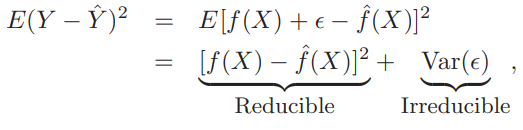
\includegraphics[scale=0.5]{images/formula.png}
\end{center}
where $E(Y - \hat{Y})^2$ represents the average, or expected value, of the squared difference between the predicted and actual value of $Y$ , and $Var(\epsilon)$ represents the variance associated with the error term $\epsilon$. 

\section{How to estimate \textit{f}: Nearest neighbor averaging}
One of the simplest methods to estimate $f$ is to compute the mean over all observations for a given $X$:
\[\hat{f}(x) = E(Y | X = x)\]
where $E(Y | X = x)$ is the expected value (average) of $Y$ given $X = x$. However, typically we have few or zero data points for an exact $X = x$, so we cannot compute $E(Y|X=x)$. Then, we can reformulate $\hat{f}$ as the average of of all the data points in some neighborhood of $x$ $\mathcal{N}(x)$:
\[\hat{f}(x) = \text{Ave}(Y | X \in \mathcal{N}(x))\]
\textbf{Nearest neighbor averaging} can be pretty good for small $p$ (low-dimensional data), i.e. $p \leq 4$. This decrease in performance as the dimension increases is a common problem for this kind of model, and results from the fact that in higher dimensions there is effectively a reduction in sample size. This is due to the so called \textbf{curse of dimensionality}, that is, the $K$ observations that are nearest to a given test observation $x$ may be very far away from $x$ in $p$-dimensional space when $p$ is large, leading to a very poor prediction of $f(x)$.
\begin{center}
    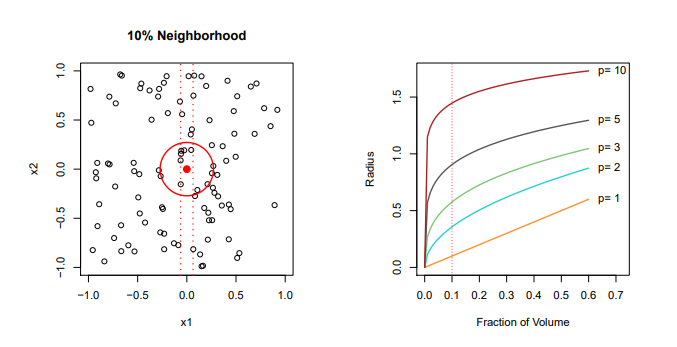
\includegraphics[]{images/curse dimensionality.png}
\end{center}
The concept is that we need to get a reasonable fraction of the $K$ values of $y_i$ to average to bring the variance down, e.g. 10\%. However, A 10\% neighborhood in high dimensions need no longer be local, so we lose the spirit of estimating $E(Y|X=x)$ by local averaging.


\section{Parametric Methods}
Parametric methods involve a two-step model-based approach.
\begin{enumerate}
    \item First, we make an assumption about the functional form, or shape, of $f$. For example, one very simple assumption is that $f$ is linear in $X$: 
    \begin{equation}
        f(X) = \beta_0 + \beta_1 X_1 + \beta_2 X_2 + ... + \beta_p X_p
        \label{linear}
    \end{equation}
    This is a \textbf{linear model}.

    \item After a model has been selected, we need a procedure that uses the training data to \textit{fit} or \textit{train} the model. In the case of the linear model \ref{linear}, we need to estimate the parameters $\beta_0, \beta_1,...,\beta_p$. That is, we want to find values of these parameters such that
    \[Y \approx \beta_0 + \beta_1 X_1 + \beta_2 X_2 + ... + \beta_p X_p\]
\end{enumerate}
The model-based approach just described is referred to as parametric;
it reduces the problem of estimating $f$ down to one of estimating a set of parameters. The potential disadvantage of a parametric approach is that the model we choose will usually not match the true unknown form of $f$.\\\\
A linear model gives a reasonable fit here:
\begin{center}
    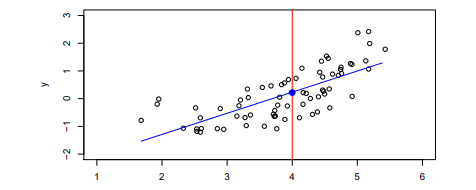
\includegraphics[]{images/linear.png}
\end{center}
A \textbf{quadratic} model $\hat{f}(X) = \beta_0 + \beta_1 X + \beta_2 X^2$ fits slightly better:
\begin{center}
    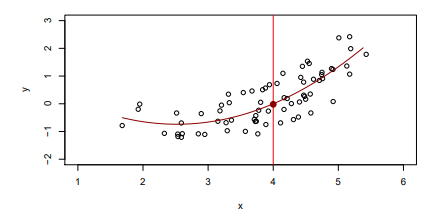
\includegraphics[]{images/quadratic.png}
\end{center}
If the chosen model is too far from the true $f$, then our estimate will be poor. We can try to address this problem by choosing \textit{flexible} models that can fit many different possible functional forms for $f$. But in general, fitting a more flexible model requires estimating a greater number of parameters. These more complex models can lead to a phenomenon known as \textbf{overfitting} the data, which essentially means they model the random noise in the training data, rather than the intended outputs.

\section{Some trade-offs}
Of the many methods that we will examine, some are less flexible, or more restrictive, in the sense that they can produce just a relatively small range of shapes to estimate $f$. For example, the linear regression presented before is a relatively inflexible approach, because it can only generate linear functions. On the other hand, other methods are more flexible.\\\\
One might reasonably ask the following question: \textit{why would we ever
choose to use a more restrictive method instead of a very flexible approach?} There are several reasons that we might prefer a more restrictive model. For example, restrictive models are much more interpretable. In contrast, very flexible approaches can lead to such complicated estimates of $f$ that it is difficult to understand how any individual predictor is associated with the response.\\\\
The figure below provides an illustration of the trade-off between flexibility and interpretability for some methods:
\begin{center}
    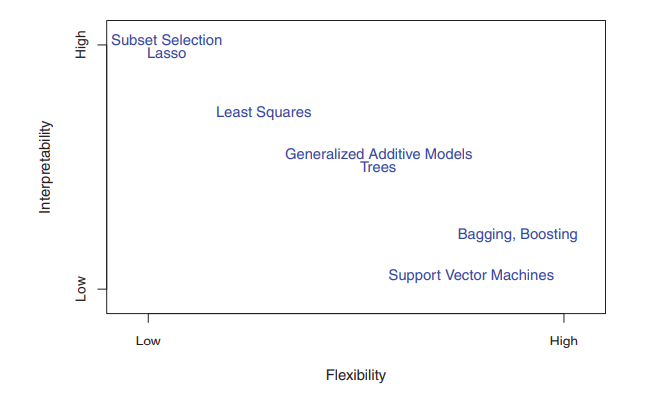
\includegraphics[scale=0.8]{images/trade-off.png}
\end{center}

\section{Assessing Model Accuracy}
In order to evaluate the performance of a statistical learning method on a given data set, we need some way to measure how well its predictions actually match the observed data. In the regression setting, the most commonly-used measure is the \textbf{mean squared error} (MSE), given by
\begin{equation}
    MSE_{Tr} = \frac{1}{n} \sum_{i=1}^n (y_i - \hat{f}(x_i))^2
    \label{MSE}
\end{equation}
The $MSE_{Tr}$ is computed using the training data that was used to fit the model, and so should more accurately be referred to as the training $MSE$. But in general, we do not really care how well the method works on the training data. Rather, we are interested in \textit{the accuracy of the predictions that we obtain when we apply our method to previously unseen test data}.\\\\
How can we go about trying to select a method that minimizes the test
$MSE_{Te}$?  In some settings, we may have a test data set available, that is,
we may have access to a set of observations that were not used to train
the statistical learning method. We can then simply evaluate \ref{MSE} on the
test observations, and select the learning method for which the test $MSE_{Te}$ is smallest. But what if no test observations are available? In that case, one might imagine simply selecting a statistical learning method that minimizes the training $MSE_{Tr}$. Unfortunately, there is a fundamental problem with this strategy: there is no guarantee that the method with the lowest training $MSE_{Tr}$ will also have the lowest test $MSE_{Te}$. The figure below illustrates this phenomenon on a simple example:
\begin{center}
    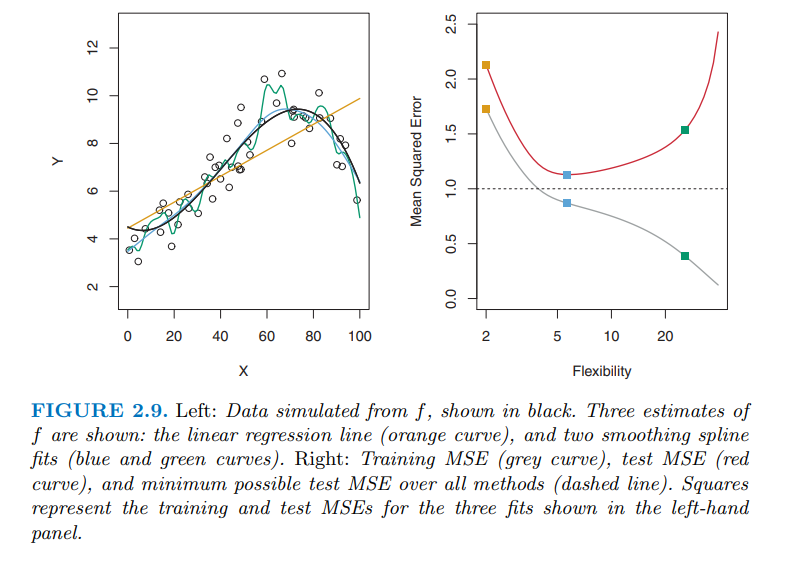
\includegraphics[scale=0.8]{images/overfit_1.png}
\end{center}
As model flexibility increases, training $MSE_{Tr}$ will decrease, but the test $MSE_{Te}$ may not. When a given method yields a small training $MSE_{Tr}$ but a large test $MSE_{Te}$, we are said to be \textit{overfitting} the data. This happens because our statistical learning procedure is working too hard to find patterns in the training data, and may be picking up some patterns that are just caused by random chance rather than by true properties of the unknown function $f$.
\begin{center}
    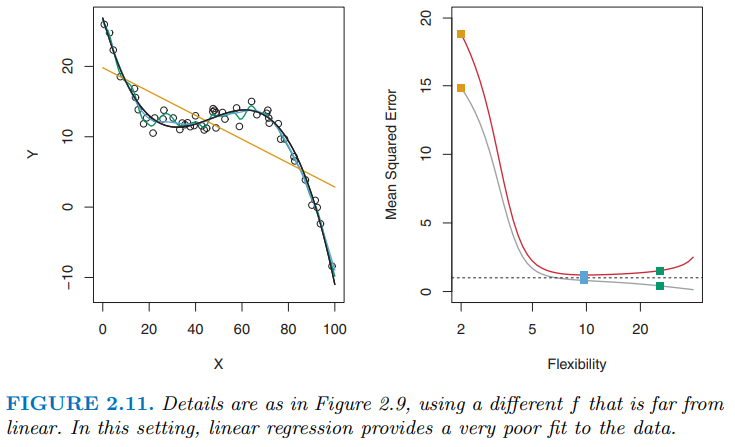
\includegraphics[scale=0.8]{images/overfit_2.png}
\end{center}
The figure above displays an example in which $f$ is highly non-linear. The
training and test $MSE_{Tr}$ curves still exhibit the same general patterns, but now there is a rapid decrease in both curves before the test $MSE_{Te}$ starts to increase slowly.\\\\
In practice, one can usually compute the training $MSE_{Tr}$ with relative
ease, but estimating test $MSE_{Te}$ is considerably more difficult because usually no test data are available. We will discuss a variety of approaches that can be used in practice to estimate $MSE_{Te}$. One important method is \textit{cross-validation}, which is a method for estimating test $MSE_{Te}$ using the training data.

\section{Bias-Variance Trade-Off}
It is possible to show that the expected test $MSE_{te}$, for a given value $x_0$, can always be decomposed into the sum of three fundamental quantities:
\begin{itemize}
    \item the variance of $\hat{f}(x_0)$,
    \item the squared bias of $\hat{f}(x_0)$,
    \item and the variance of the error term $\epsilon$
\end{itemize}
\begin{equation}
    E(y_0 - \hat{f}(x_0))^2 = \text{Var}(\hat{f}(x_0)) + [\text{Bias}(\hat{f}(x_0))]^2 + \text{Var}(\epsilon)
    \label{bias-variance}
\end{equation}
Equation \ref{bias-variance} refers to the average test $MSE_{Te}$ that we would obtain if we repeatedly estimated $f$ using a large number of training sets, and tested each at $x_0$.\\\\
Equation \ref{bias-variance}  tells us that in order to minimize the expected test error, we need to select a statistical learning method that simultaneously achieves low variance and low bias. What do we mean by the variance and bias of a statistical learning method?\\\\
Variance refers to the amount by which $\hat{f}$ would change if we estimated it using a different training data set. Ideally, the estimate for $f$ should not vary too much between training sets. However, if a method has high variance, then small changes in the training data can result in large changes in $\hat{f}$. In general, more flexible statistical methods have higher variance.\\\\
On the other hand, bias refers to the error that is introduced by approximating a real-life problem, which may be extremely complicated, by a much simpler model.\\\\
As a general rule, as we use more flexible methods, the variance will increase and the bias will decrease. The relative rate of change of these two quantities determines whether the test MSE increases or decreases. Therefore, we need to choose the flexibility based on average test error amounts to a bias-variance trade-off. As we increase the flexibility of a class of methods, the bias tends to initially decrease faster than the variance increases. Consequently, the expected test $MSE_{Te}$ declines. However, at some point increasing flexibility has little impact on the bias but starts to significantly increase the variance. When this happens the test $MSE_{Te}$ increases following the $U$-shape curve presented in the figures above.

\chapter{Lec 06 - Linear Regression}

\section{Linear Regression}
Linear regression is a simple approach to supervised learning. It assumes that the dependence of $Y$ on $X_1, X_2, . . . X_p$ is linear. Although it may seem overly simplistic, linear regression is extremely useful both conceptually and practically. Consider the following advertising data:
\begin{center}
    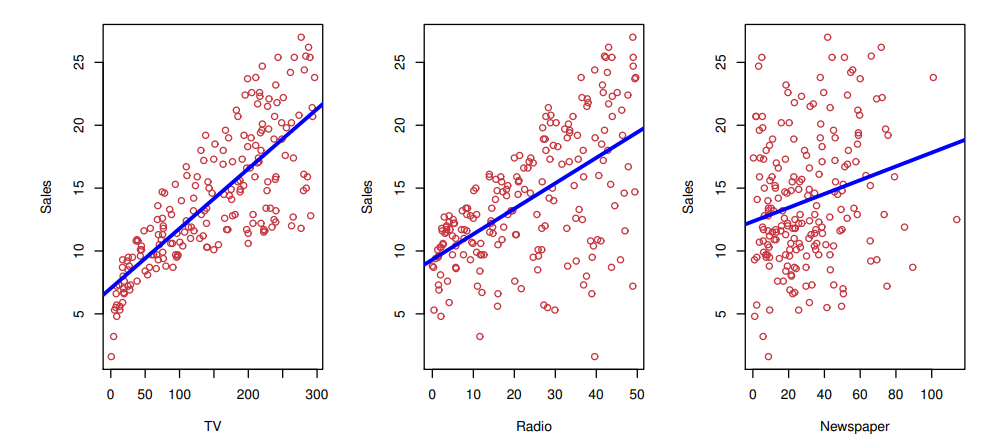
\includegraphics[scale=0.7]{images/advertising_lr.png}
\end{center}
Suppose that in our role as statistical consultants we are asked to suggest, on the basis of this data, a marketing plan for next year that will result in high product sales. What information would be useful in order to provide such a recommendation? Here are a few important questions that we might seek to address:
\begin{enumerate}
    \item Is there a relationship between advertising budget and sales?

    \item How strong is the relationship between advertising budget and sales?

    \item Which media contribute to sales?

    \item How accurately can we predict future sales?

    \item Is the relationship linear?

    \item Is there synergy among the advertising media?
\end{enumerate}
\textit{Simple linear regression} lives up to its name: it is a very straightforward approach for predicting a quantitative response $Y$ on the basis of a single predictor variable $X$. It assumes that there is approximately a linear relationship between $X$ and $Y$. Mathematically, we can write this linear relationship as:
\[Y \approx \beta_0 + \beta_1 X\]
For example, $X$ may represent TV advertising and $Y$ may represent sales. $\beta_0$ and $\beta_1$ are two unknown constants that represent
the \textit{intercept} and \textit{slope} terms in the linear model. Together, $\beta_0$ and $\beta_1$ are known as the model \textit{coefficients} or \textit{parameters}. Once we have used our training data to produce estimates $\hat{\beta}_0$ and $\hat{\beta}_1$ for the model coefficients, we can predict future sales on the basis of a particular value of TV advertising by computing
\[\hat{y} = \hat{\beta}_0 + \hat{\beta}_1 x\]
where $\hat{y}$ indicates a prediction of $Y$ on the basis of $X = x$.

\section{Estimating the Coefficients}
Let $\{(x_1, y_1), (x_2, y_2), ..., (x_n, y_n)\}$ be the $n$ observation pairs. Let $\hat{y}_i = \hat{\beta}_0 + \hat{\beta}_1 x_i$ be the prediction for $Y$ based on the $i$-th value of $X$. Then $e_i = y_i - \hat{y}_i$ represents the $i$-th residual, that is,  the difference between the $i$-th observed response value and the $i$-th response value that is predicted by our linear model. We define the residual sum of squares (RSS) as
\[\text{RSS} = e_1^2 + e_2^2 + ... + e_n^2\]
or equivalently as
\[\text{RSS} = (y_1 - \hat{\beta}_0 + \hat{\beta}_1 x_1)^2 + (y_2 - \hat{\beta}_0 + \hat{\beta}_1 x_2)^2 + ... + (y_n - \hat{\beta}_0 + \hat{\beta}_1 x_n)^2\]
The least squares approach chooses $\hat{\beta}_0$ and $\hat{\beta}_1$ to minimize the RSS. Using some calculus, one can show that the minimizers are
\[
\begin{split}
    \hat{\beta}_1 = & \frac{\sum_{i=1}^n (x_i - \overline{x}) (y_i - \overline{y})}{\sum_{i=1}^n (x_i - \overline{x})^2} \\
    \hat{\beta}_0 = & \overline{y} - \hat{\beta}_1 \overline{x}
\end{split}
\]
where $\overline{y} \equiv \frac{1}{n}\sum_{i=1}^n y_i$ and $\overline{x} \equiv \frac{1}{n}\sum_{i=1}^n x_i$ are the sample means.
\begin{center}
    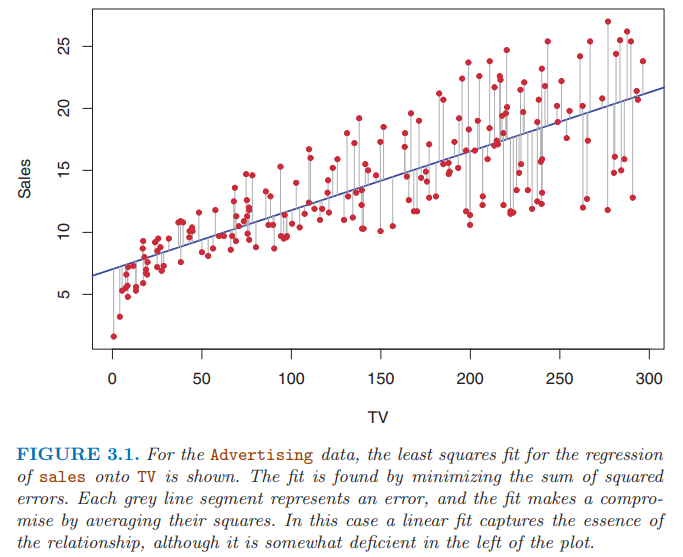
\includegraphics[scale=0.8]{images/linear_reg adv.png}
\end{center}

\section{Assessing the Accuracy of the Coefficient Estimates}
Recall that we assume that the true relationship between $X$ and $Y$ takes the form $Y = f(X) + \epsilon$ for some unknown function $f$, where $\epsilon$ is a mean-zero random error term. If $f$ is to be approximated by a linear function, then we can write this relationship as
\begin{equation}
    Y = \beta_0 + \beta_1X + \epsilon
    \label{pop_regr}
\end{equation}
Here $\beta_0$ is the intercept term, that is, the expected value of $Y$ when $X = 0$,
and $\beta_1$ is the slope, the average increase in $Y$ associated with a one-unit increase in $X$.\\\\
The model given by \ref{pop_regr} defines the \textit{population regression line}, which is the best linear approximation to the true relationship between $X$ and $Y$. The least squares regression coefficient estimates characterize the \textit{least squares line}.
\begin{center}
    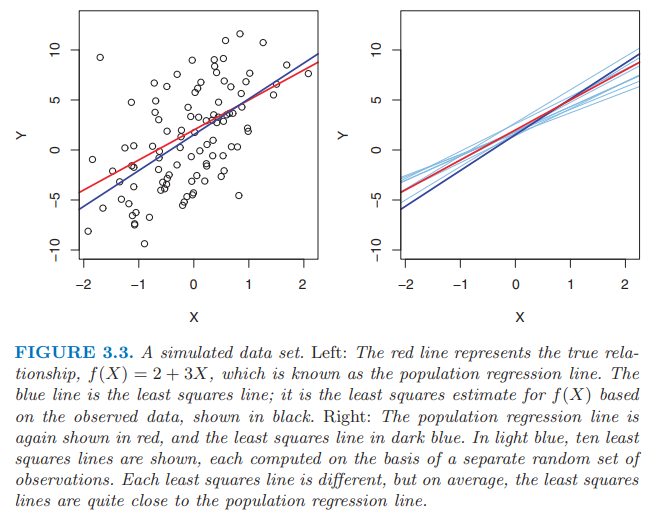
\includegraphics[scale=0.8]{images/pop_reg vs lsr.png}
\end{center}
At first glance, the difference between the population regression line and the least squares line may seem subtle and confusing. We only have one data set, and so what does it mean that two different lines describe the relationship between the predictor and the response? Fundamentally, the concept of these two lines is a natural extension of the standard statistical approach of using information from a sample to estimate characteristics of a large population.\\\\
For example, suppose that we are interested in knowing the population mean $\mu$ of some random variable $Y$.  Unfortunately, $\mu$ is unknown, but we do have access to $n$ observations from $Y$, which we can write as $y_1,...,y_n$, and which we can use to estimate $\mu$. A reasonable estimate is $\hat{\mu} = \overline{y}$, where $\overline{y} = \frac{1}{n}\sum_{i=1}^n y_i$ is the sample mean. The sample mean and the population mean are different, but in general the sample mean will provide a good estimate of the population mean. In the same way, the unknown coefficients $\beta_0$ and $\beta_1$ in linear regression define the population regression line. We seek to estimate these unknown coefficients using $\hat{\beta}_0$ and $\hat{\beta}_1$.\\\\
We continue the analogy with the estimation of the population mean
$\mu$ of a random variable $Y$. A natural question is as follows: how accurate is the sample mean $\hat{\mu}$ as an estimate of $\mu$?  the average of $\hat{\mu}$’s over many data sets will be very close to $\mu$, but that a single estimate $\hat{\mu}$ may be a substantial underestimate or overestimate of $\mu$. How far off will that single estimate of $\hat{\mu}$ be?  In general, we answer this question by computing the standard error of $\hat{\mu}$, written as $\text{SE}(\hat{\mu})$.
\[\text{Var}(\hat{\mu}) = \text{SE}(\hat{\mu})^2 = \frac{\sigma^2}{n}\]
Roughly speaking, the standard error tells us the average amount that this estimate $\hat{\mu}$ differs from the actual value of $\mu$. In a similar vein, we can wonder how close $\hat{\beta}_0$
and $\hat{\beta}_1$ are to the true values $\beta_0$ and $\beta_1$. To compute the standard errors
associated with $\hat{\beta}_0$ and $\hat{\beta}_1$, we use the following formulas:
\[\text{SE}(\hat{\beta}_0)^2 = \sigma^2 \left[ \frac{1}{n} + \frac{\overline{x}^2}{\sum_{i=1}^n (x_i - \overline{x})^2}\right], \quad \text{SE}(\hat{\beta}_1)^2 = \frac{\sigma^2}{\sum_{i=1}^n (x_i - \overline{x})^2}\]
where $\sigma^2 = \text{Var}(\epsilon)$\\\\
Standard errors can be used to compute confidence intervals. A 95\% confidence interval is defined as a range of values such that with 95\% probability, the range will contain the true unknown value of the parameter. For linear regression, the 95\% confidence interval for $\beta_1$
approximately takes the form
\[\hat{\beta}_1 \pm 2 \cdot \text{SE}(\hat{\beta}_1)\]
That is, there is approximately a 95\% chance that the interval
\[\left[\hat{\beta}_1 - 2 \cdot \text{SE}(\hat{\beta}_1), \,\, \hat{\beta}_1 + 2 \cdot \text{SE}(\hat{\beta}_1)\right]\]
will contain the true value of $\beta_1$. Similarly, a confidence interval for $\beta_0$ approximately takes the form
\[\hat{\beta}_0 \pm 2 \cdot \text{SE}(\hat{\beta}_0)\]
For the advertising data, the 95\% confidence interval for $\beta_1$ is $[0.042, 0.053]$.\\\\
Standard errors can also be used to perform hypothesis tests on the coefficients. The most common hypothesis test involves testing the \textit{null hypothesis} of
\[H_0 \,\, :\,\, \text{There is no relationship between $X$ and $Y$}\]
versus the \textit{alternative hypothesis}
\[H_A \,\, : \,\, \text{There is some relationship between $X$ and $Y$}\]
Mathematically, this corresponds to testing
\[H_0 \,\, : \,\, \beta_1 = 0\]
versus
\[H_A \,\, : \,\, \beta_1 \neq 0\]
since if $\beta_1 = 0$ then the model reduces to $Y = \beta_0 + \epsilon$, and $X$ is
not associated with $Y$. To test the null hypothesis, we need to determine whether $\hat{\beta}_1$, our estimate for $\beta_1$, is sufficiently far from zero that we can be confident that $\beta_1$ is non-zero. How far is far enough? This of course depends on the accuracy of $\hat{\beta}_1$, that is, it depends on $\text{SE}(\hat{\beta}_1)$. If $\text{SE}(\hat{\beta}_1)$ is small, then even relatively small values of $\hat{\beta}_1$ may provide strong evidence that $\beta_1 \neq 0$, and hence that there is a relationship between $X$ and $Y$. In contrast, if $\text{SE}(\hat{\beta}_1)$ is large, then $\hat{\beta}_1$ must be large in absolute value in order for us to reject the null hypothesis. In practice, we compute a $t$-statistic, given by
\begin{equation}
    t = \frac{\hat{\beta}_1 - 0}{\text{SE}(\hat{\beta}_1)}
    \label{t-stat}
\end{equation}
which measures the number of standard deviations that $\hat{\beta}_1$ is away from 0. If there really is no relationship between $X$ and $Y$ (i.e. assuming $\beta_1 = 0$), then we expect that \ref{t-stat} will have a $t$-distribution with $n - 2$ degrees of freedom.
\begin{center}
    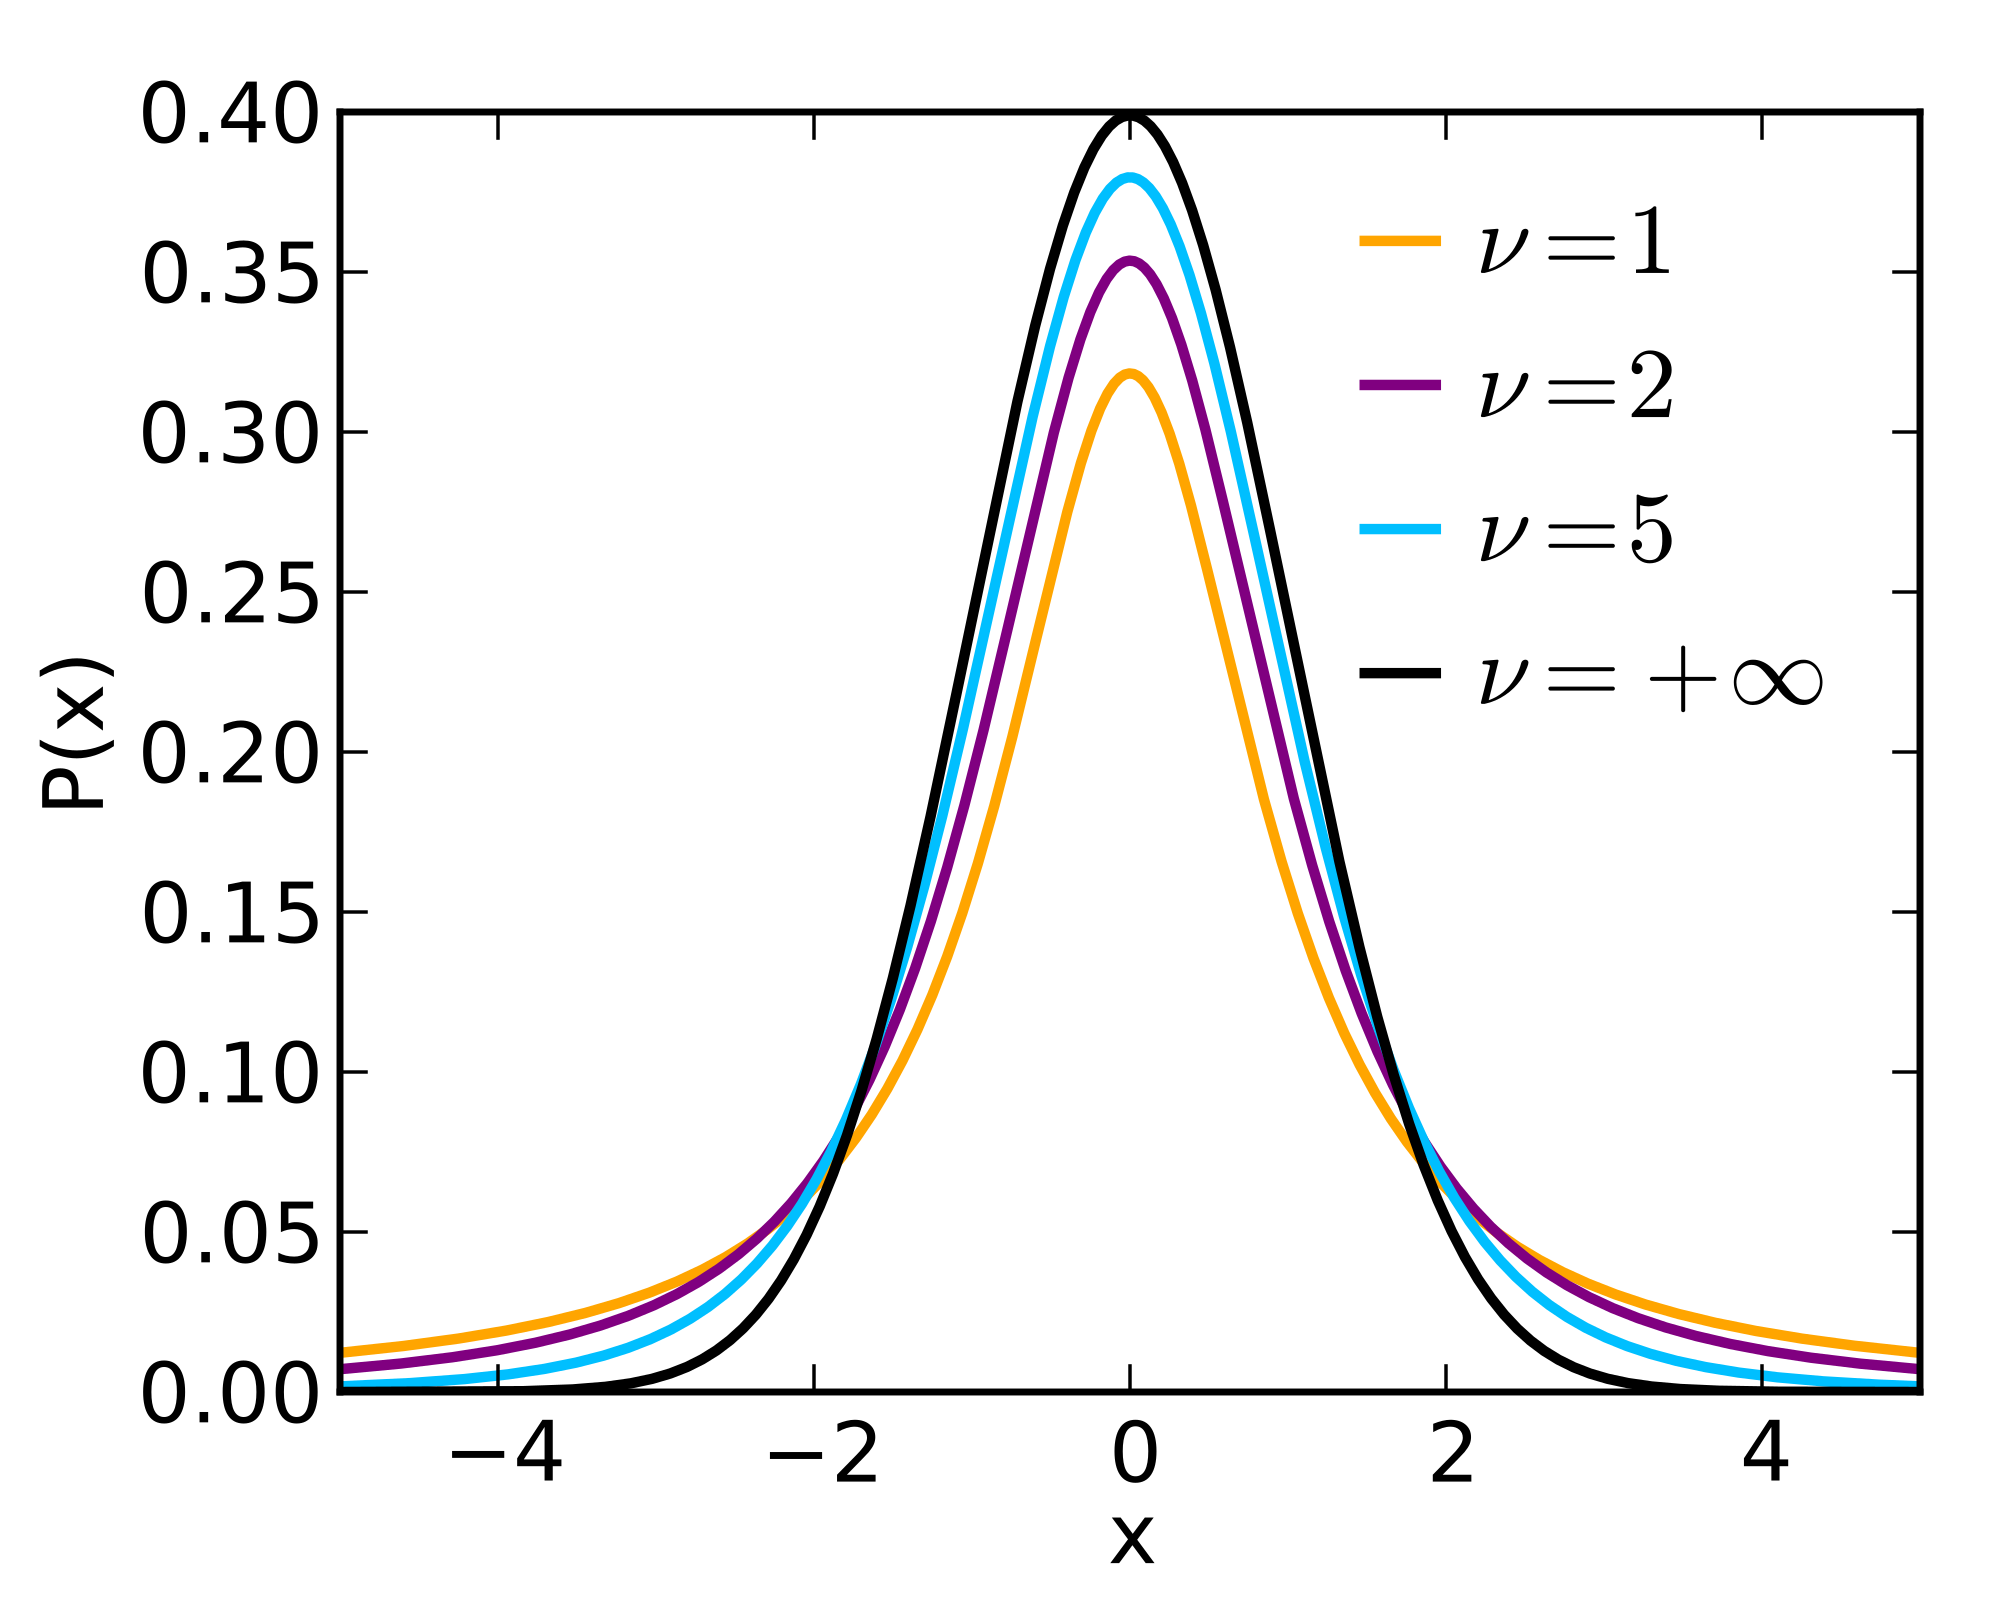
\includegraphics[scale=0.1]{images/t-distr.png}
\end{center}
The $t$-distribution has a bell shape and for values of $n$ greater than approximately 30 it is quite similar to the normal distribution. Consequently, it is a simple matter to compute the probability of observing any value equal to $|t|$ or larger, \textbf{assuming} $\beta_1 = 0$. We call this probability the $p$-value, which we can interpret as follows: \textit{which is the probability that the true $\beta_1$ is 0 if our estimate $\hat{\beta}_1$ is far from 0 according to $t$?} Note that if $\hat{\beta}_1$ is very close to 0 and/or $\text{SE}(\hat{\beta})_1$ is very high, then $t$ will be higher, and so the $p$-value. In contrast, if $\hat{\beta}_1$ is far from 0 and/or the standard error is very low, the $p$-value will be low.
\\\\
Hence, if we see a small $p$-value, then we can infer that there is an association between the predictor and the response. We reject the null hypothesis, that is, we declare a relationship to exist between $X$ and $Y$, if the $p$-value is small enough. Typical $p$-value cutoffs for rejecting the null hypothesis are 5 or 1\%.
\begin{center}
    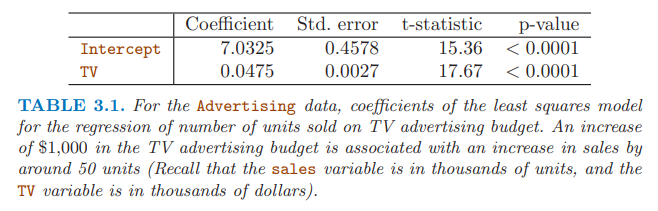
\includegraphics[scale=0.8]{images/p-value table.png}
\end{center}


\chapter{Lec 07 - 08 - Linear Regression II}

\section{$R^2$ Statistic}
The $R^2$ statistic provides a measure of lack of fit of the linear model to the data. It takes the form of a proportion, the proportion of variance explained, and so it always takes on a value between 0 and 1, and is independent of the scale of $Y$. To calculate $R^2$, we use the formula
\[R^2 = \frac{TSS - RSS}{TSS} = 1 - \frac{RSS}{TSS}\]
where
\[TSS = \sum_{i=1}^n (y_i - \bar{y})^2 \quad RSS = \sum_{i=1}^n (y_i - \hat{y}_i)^2\]
TSS (total sum of squares) measures the total variance in the response $Y$, and can be  thought of as the amount of variability inherent in the response before the regression is performed \footnote{note that TSS corresponds to the best prediction we can do without having features}. In contrast, RSS measures the amount of variability that is left unexplained after performing the regression. Hence, TSS - RSS measures the amount of variability in the response that is explained (or removed) by performing the regression, and $R^2$ measures the proportion of variability in $Y$ that can be explained using $X$.\\\\
An $R^2$ statistic that is close to 1 indicates that a large proportion of the variability in the response has been explained by the regression. A number near 0 indicates that the
regression did not explain much of the variability in the response; this might occur because the linear model is wrong, or the inherent error $\sigma^2$ is high, or both.\\\\
This can also be seen by looking at the formulas of TSS and RSS. In particular, RSS can be written as
\[RSS = \sum_{i=1}^n (y_i - (\hat\beta_0 + \hat\beta_1 x_i))^2\]
Recall that $\hat\beta_0$ and $\hat\beta_1$ are estimated in the following way:
\[
\begin{split}
    \hat{\beta}_1 = & \frac{\sum_{i=1}^n (x_i - \overline{x}) (y_i - \overline{y})}{\sum_{i=1}^n (x_i - \overline{x})^2} \\
    \hat{\beta}_0 = & \overline{y} - \hat{\beta}_1 \overline{x}
\end{split}
\]
Then, if $\hat\beta_1 = 0$, which means no correlation between $X$ and $Y$, the RSS formula becomes
\[RSS = \sum_{i=0}^n (y_i - \hat\beta_0)^2 = \sum_{i=0}^n (y_i - \overline{y})^2 = TSS\]
The $R^2$ statistic is a measure of the linear relationship between $X$ and
$Y$. Recall that correlation, defined as
\[\text{Cor}(X,Y) = \frac{\sum_{i=1}^n (x_i - \overline{x})(y_i - \overline{y})}{\sqrt{\sum_{i=1}^n (x_i - \overline{x})^2} \sqrt{\sum_{i=1}^n (y_i - \overline{y})^2}}\]
It can be shown that in the \textit{simple linear regression} setting, $R^2 = \text{Cor}(X,Y)^2$. In other words, the squared correlation and the $R^2$ statistic are identical. However, in the multiple linear regression problem, in which we use several predictors simultaneously to predict the response, this equality does not hold.

\section{Multiple Linear Regression}
Simple linear regression is a useful approach for predicting a response on the basis of a single predictor variable. However, in practice we often have more than one predictor. One option is to run three separate simple linear regressions, each of which uses a different advertising medium as a predictor. However, this approach is not entirely satisfactory.\\\\
Instead of fitting a separate simple linear regression model for each predictor, a better approach is to extend the simple linear regression model so that it can directly accommodate multiple predictors. We can do this by giving each predictor a separate slope coefficient in a single model. In general, suppose that we have $p$ distinct predictors. Then the multiple linear regression model takes the form
\[Y = \beta_0 + \beta_1 X_1 + \beta_2 X_2 + ... + \beta_p X_p + \epsilon\]
We interpret $\beta_j$ as the average effect on $Y$ of a one unit increase in $X_j$, holding all other predictors fixed. Given estimates $\hat\beta_0, \hat\beta_1, . . . \hat\beta_p$, we can make predictions using the formula
\[\hat{y} = \hat\beta_0 + \hat\beta_1 x_1 + \hat\beta_2 x_2 + ... + \hat\beta_p x_p\]
As we did for the simple linear model, we estimate $\beta_0, \beta_1, . . . , \beta_p$ as the values that minimize the sum of squared residuals $RSS = \sum_{i=1}^n (y_i - \hat{y}_i)^2$.
This is done using standard statistical software. The values $\hat\beta_0, \hat\beta_1, . . . \hat\beta_p$ that minimize RSS are the multiple least squares regression coefficient estimates.

\subsection{Example: Qualitative Predictors}
In our discussion so far, we have assumed that all variables in our linear
regression model are quantitative. But in practice, this is not necessarily
the case; often some predictors are qualitative.\\\\
Suppose that we wish to investigate differences in credit card balance between males and females. If a qualitative predictor (also known as a \textit{factor}) only has two \textit{levels}, or possible values, then incorporating it into a regression model is very simple. We simply create an indicator or dummy variable that takes on two possible numerical values. For example, based on the gender variable, we can create a new variable that takes the form
\[
x_i = 
\begin{cases}
    1 & \text{if $i$-th person is female}\\
    0 & \text{if $i$-th person is male}
\end{cases}
\]
and use this variable as a predictor in the regression equation. This results
in the model
\[y_i = \beta_0 + \beta_1 x_i + \epsilon_i = 
\begin{cases}
    \beta_0 + \beta_1 + \epsilon_i & \text{if $i$-th person is female}\\
    \beta_0 + \epsilon_i & \text{if $i$-th person is male}
\end{cases}
\]
Now $\beta_0$ can be interpreted as the average credit card balance among males, $\beta_0 + \beta_1$ as the average credit card balance among females, and $\beta_1$ as the average difference in credit card balance between females and males.
\begin{center}
    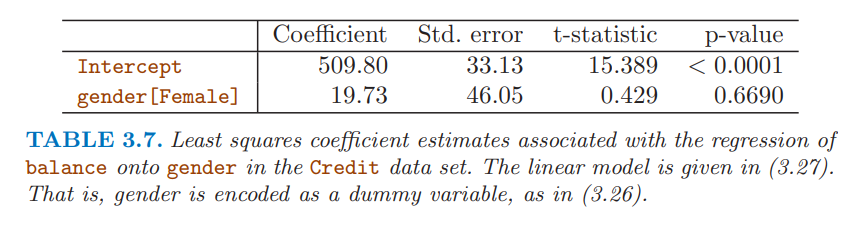
\includegraphics[scale=0.8]{images/dummy_var_1.png}
\end{center}
In the table above we can see that the average credit card debt for males is
estimated to be \$509.80, whereas females are estimated to carry \$19.73 in
additional debt for a total of \$509.80 + \$19.73 = \$529.53. However, we
notice that the p-value for the dummy variable is very high. This indicates
that there is no statistical evidence of a difference in average credit card balance between the genders.\\\\
The decision to code females as 1 and males as 0 is arbitrary, and has no effect on the regression fit, but does alter the interpretation of the coefficients.  If we had coded males as 1 and females as 0, then the estimates for $\beta_0$ and $\beta_1$ would have been 529.53 and -19.73, respectively, leading once again to a prediction of credit card debt of \$529.53 - \$19.73 = \$509.80 for males and a prediction of \$529.53 for females. Alternatively, instead of a 0/1 coding scheme, we could create a dummy variable
\[
x_i = 
\begin{cases}
    1 & \text{if $i$-th person is female}\\
    -1 & \text{if $i$-th person is male}
\end{cases}
\]
and use this variable in the regression equation. This results in the model
\[y_i = \beta_0 + \beta_1 x_i + \epsilon_i = 
\begin{cases}
    \beta_0 + \beta_1 + \epsilon_i & \text{if $i$-th person is female}\\
    \beta_0 - \beta_1 +  \epsilon_i & \text{if $i$-th person is male}
\end{cases}
\]
Now $\beta_0$ can be interpreted as the overall average credit card balance (ignoring the gender effect), and $\beta_1$ is the amount that females are above the average and males are below the average. It is important to note that the final predictions for the credit balances of males and females will be identical regardless of the coding scheme used.\\\\
When a qualitative predictor has \textbf{more} than two levels, a single dummy variable cannot represent all possible values. In this situation, we can create additional dummy variables. For example, for the ethnicity variable we create two dummy variables. The first could be
\[
x_{i1} = 
\begin{cases}
    1 & \text{if $i$-th person is Asian}\\
    0 & \text{if $i$-th person is not Asian}
\end{cases}
\]
and the second could be
\[
x_{i2} = 
\begin{cases}
    1 & \text{if $i$-th person is Caucasian}\\
    0 & \text{if $i$-th person is not Caucasian}
\end{cases}
\]
Then both of these variables can be used in the regression equation, in
order to obtain the model
\[y_i = \beta_0 + \beta_1 x_{i1} + \beta_2x_{i2} + \epsilon_i = 
\begin{cases}
    \beta_0 + \beta_1 + \epsilon_i & \text{if $i$-th person is Asian}\\
    \beta_0 + \beta_2 + \epsilon_i & \text{if $i$-th person is Caucasian}\\
    \beta_0 + \epsilon_i & \text{if $i$-th person is African American}
\end{cases}
\]
Now $\beta_0$ can be interpreted as the average credit card balance for African Americans, $\beta_1$ can be interpreted as the difference in the average balance between the Asian and African American categories, and $\beta_2$ can be interpreted as the difference in the average balance between the Caucasian and African American categories. There will always be one fewer dummy variable than the number of levels. The level with no dummy variable, African American in this example, is known as the baseline.

\section{Predictions}
Once we have fit the multiple regression model, it is straightforward to apply it in  order to predict the response $Y$ on the basis of a set of values for the predictors $X_1, X_2,...,X_p$. However, there are three sorts of uncertainty associated with this prediction.
\begin{enumerate}
    \item The coefficient estimates $\hat\beta_0, \hat\beta_1,..., \hat\beta_p$ are estimates for $\beta_0, \beta_1,...,\beta_p$. That is, the \textit{least squares plane}
    \[\hat{Y} = \hat\beta_0 + \hat\beta_1 X_1 + \hat\beta_2 X_2 + ... + \hat\beta_p X_p + \epsilon\]
    is only an estimate for the true population regression plane
    \[f(X) = \beta_0 + \beta_1 X_1 + \beta_2 X_2 + ... + \beta_p X_p + \epsilon\]
    The inaccuracy in the coefficient estimates is related to the reducible error.

    \item Of course, in practice assuming a linear model for $f(X)$ is almost always an approximation of reality, so there is an additional source of potentially reducible error which we call \textit{model bias}.

    \item  Even if we knew $f(X)$, that is, even if we knew the true values for $\beta_0, \beta_1,...,\beta_p$, the response value cannot be predicted perfectly because of the random error $\epsilon$ (irreducible error).
\end{enumerate}

\section{Extensions of the Linear Model}

\subsection{Non-linear Relationships}
As discussed previously, the linear regression model assumes a linear relationship between the response and predictors. But in some cases, the true relationship between the response and the predictors may be nonlinear. Here we present a very simple way to directly extend the linear model to accommodate non-linear relationships, using \textit{polynomial regression}.
\begin{center}
    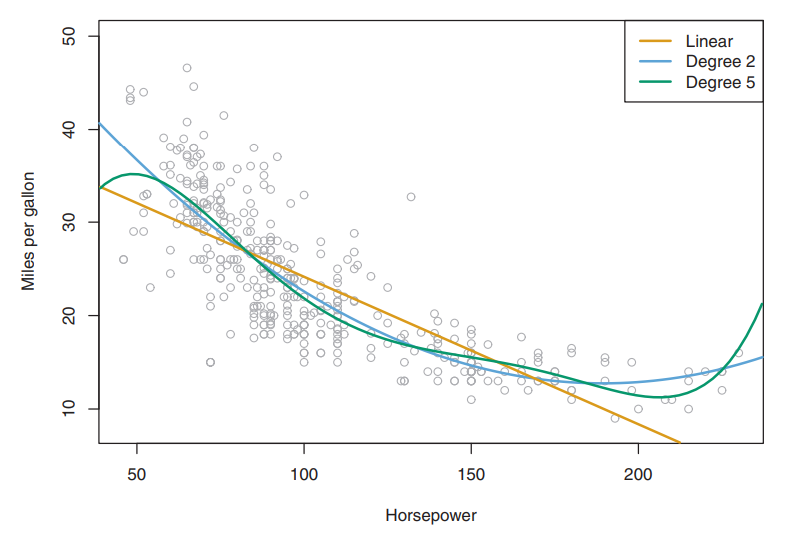
\includegraphics[scale=0.8]{images/pol-reg.png}
\end{center}
Consider the figure above,  in which the mpg (gas mileage in miles per gallon) versus horsepower is shown for a number of cars in the Auto data set. The orange line represents the linear regression fit. There is a pronounced relationship between mpg and horsepower, but it seems clear that this relationship is in fact non-linear: the data suggest a curved relationship. A simple approach for incorporating non-linear associations in a linear model is to include transformed versions of the predictors in the model.\\\\
For example, the points in the figure seem to have a quadratic shape, suggesting that a model of the form
\[mpg = \beta_0 + \beta_1 \times horsepower + \beta_2 \times horsepower^2 + \epsilon\]
may provide a better fit. It involves predicting mpg using a
non-linear function of horsepower. But it is still a linear model! That is, it is simply a multiple linear regression model with $X_1 = horsepower$ and $X_2 = horsepower^2$. So we can use standard linear regression software to estimate $\beta_0, \beta_1$, and $\beta_2$ in order to produce a non-linear fit.\\\\
The blue curve shows the resulting quadratic fit to the data. The quadratic fit appears to be substantially better than the fit obtained when just the linear term is included. The $R^2$ of the quadratic fit is 0.688, compared to 0.606 for the linear fit.\\\\
If including $horsepower^2$ led to such a big improvement in the model, why not include $horsepower^3$, $horsepower^4$, or even $horsepower^5$? The green curve displays the fit that results from including all polynomials up to fifth degree. The resulting fit seems unnecessarily wiggly—that is, it is unclear that including the additional terms really has led to a better fit to the data. 

\subsection{Removing the Additive Assumption}
Consider the standard linear regression model with two variables,
\[Y = \beta_0 + \beta_1 X_1 + \beta_2 X_2 + \epsilon\]
According to this model, if we increase $X_1$ by one unit, then $Y$ will increase by an average of $\beta_1$ units. Notice that the presence of $X_2$ does not alter this statement, that is, regardless of the value of $X_2$, a one-unit increase in $X_1$ will lead to a $\beta_1$-unit increase in $Y$.\\\\
One way of extending this model to allow for interaction effects is to include a third predictor, called an \textit{interaction term}, which is constructed by computing the product of $X_1$ and $X_2$. This results in the model
\[Y = \beta_0 + \beta_1 X_1 + \beta_2 X_2 + \beta_3 X_1X_2 + \epsilon\]
How does inclusion of this interaction term relax the additive assumption? Note that the equation above can be rewritten as
\[Y = \beta_0 +  (\beta_1 + \beta_3X_2)X_1 + \beta_2X_2 + \epsilon\]
Note that the effect of $X_1$ on $Y$ is no longer constant: adjusting $X_2$ will change the impact of $X_1$ on $Y$. For example, suppose that we are interested in studying the productivity of a factory. We wish to predict the number of units produced on the basis of the number of production lines and the total number of workers.\\\\
It seems likely that the effect of increasing the number of production lines will depend on the number of workers, since if no workers are available to operate the lines, then increasing the number of lines will not increase production. This suggests that it would be appropriate to include an interaction term between lines and workers in a linear model to predict units. Suppose that when we fit the model, we obtain
\[
\begin{split}
    units & \approx 1.2+3.4 \times lines + 0.22 \times workers + 1.4 \times (lines \times workers)\\
    & = 1.2 + (3.4+1.4 \times workers) \times lines + 0.22 \times workers.
\end{split}
\]
In other words, adding an additional line will increase the number of units produced by $3.4+1.4 \times workers$. Hence the more workers we have, the stronger will be the effect of lines.\\\\
Consider the Credit data set example we already seen, and suppose that we wish to predict balance using the income (quantitative) and student (qualitative) variables. In the absence of an interaction term, the model takes the form
\[
\begin{split}
    balance_i & \approx \beta_0 + \beta_1 \times income_i + \begin{cases}
    \beta_2 & \text{if $i$-th person is a student}\\
    0 & \text{otherwise}
\end{cases}\\
    & = \beta_1 \times income_i + \begin{cases}
        \beta_0 + \beta_2 & \text{if $i$-th person is a student}\\
        \beta_0 & \text{otherwise}
    \end{cases}
\end{split}
\]
Notice that this amounts to fitting two parallel lines to the data, one for students and one for non-students. The lines for students and non-students have different intercepts, $\beta_0 + \beta_2$ versus $\beta_0$, but the same slope, $\beta_1$.
\begin{center}
    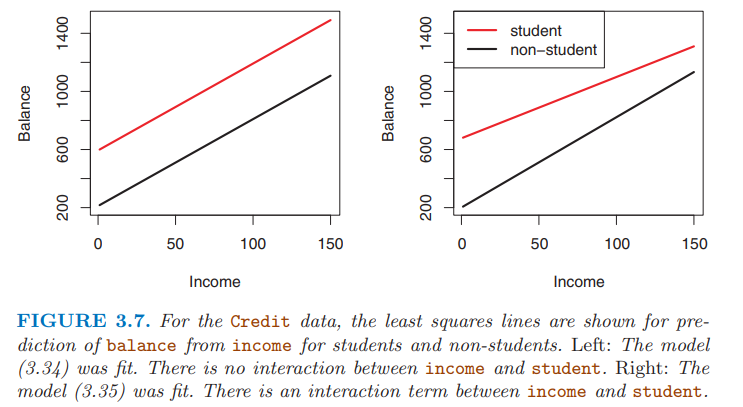
\includegraphics[scale=0.8]{images/creadit card ex. additive.png}
\end{center}
The fact that the lines are parallel means that the average effect on balance of a one-unit increase in income does not depend on whether or not the individual is a student. This represents a potentially serious limitation of the model, since in fact a change in income may have a very different effect on the credit card balance of a student versus a non-student.\\\\
This limitation can be addressed by adding an interaction variable, created by multiplying income with the dummy variable for student. Our model now becomes
\[
\begin{split}
    balance_i & \approx \beta_0 + \beta_1 \times income_i + \begin{cases}
    \beta_2 + \beta_3 \times income_i & \text{if student}\\
    0 & \text{otherwise}
\end{cases}\\
    & = \begin{cases}
        (\beta_0 + \beta_2)+(\beta_1 + \beta_3) \times income_i & \text{if student}\\
        \beta_0 + \beta_1 \times income_i & \text{otherwise}
    \end{cases}
\end{split}
\]
Once again, we have two different regression lines for the students and the non-students. But now those regression lines have different intercepts, $\beta_0+\beta_2$ versus $\beta_0$, as well as different slopes, $\beta_1+\beta_3$ versus $\beta_1$. This allows for the possibility that changes in income may affect the credit card balances of students and non-students differently.\\\\
From the right panel of the figure above we note that the slope for students is lower than the slope for non-students. This suggests that increases in income are associated with smaller increases in credit card balance among students as compared to non-students.

\section{Potential Problems}
When we fit a linear regression model to a particular data set, many problems may occur. Most common among these are the following:
\begin{enumerate}
    \item Non-linearity of the response-predictor relationships.
    \item Correlation of error terms.
    \item Non-constant variance of error terms.
    \item Outliers.
    \item High-leverage points.
    \item Collinearity.
\end{enumerate}

\subsection{Non-linearity of the response-predictor relationships}
The linear regression model assumes that there is a straight-line relationship between the predictors and the response. If the true relationship is far from linear, then virtually all of the conclusions that we draw from the fit are suspect. In addition, the prediction accuracy of the model can be significantly reduced.
\\\\
Residual plots are a useful graphical tool for identifying non-linearity. Given a simple linear regression model, we can plot the residuals, $e_i = y_i - \hat{y}_i$, versus the predictor $x_i$. In the case of a multiple regression model, since there are multiple predictors, we instead plot the residuals versus the predicted (or fitted) values $\hat{y}_i$. Ideally, the residual plot will show no  discernible pattern. The presence of a pattern may indicate a problem with some aspect of the linear model.
\begin{center}
    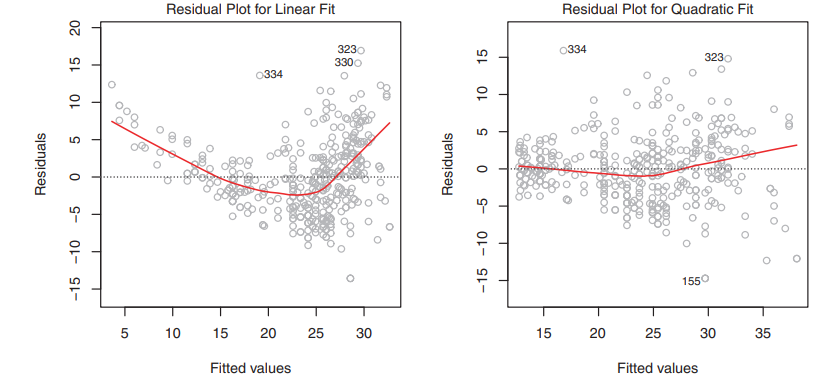
\includegraphics[scale=0.8]{images/residual-plot.png}
\end{center}

\subsection{Correlation of Error Terms}
An important assumption of the linear regression model is that the error terms, $\epsilon_1, \epsilon_2,...,\epsilon_n$, are uncorrelated. What does this mean? For instance, if the errors are uncorrelated, then the fact that $\epsilon_i$ is positive provides little or no information about the sign of $\epsilon_{>i+1}$. The standard errors that are computed for the estimated regression coefficients or the fitted values are based on the assumption of uncorrelated error terms. However, if the error terms are correlated, we may have an unwarranted sense of confidence in our model. Such correlations frequently occur in the context of time series data, which consists of observations for which measurements are obtained at discrete points in time.

\subsection{Non-constant Variance of Error Terms}
Another important assumption of the linear regression model is that the error terms have a constant variance, $\text{Var}(\epsilon_i) = \sigma^2$. The standard errors, confidence intervals, and hypothesis tests associated with the linear model rely upon this assumption.\\\\
Unfortunately, it is often the case that the variances of the error terms are non-constant. For instance, the variances of the error terms may increase with the value of the response. One can identify non-constant variances in the errors, or heteroscedasticity, from the presence of a funnel shape in the residual plot.
\begin{center}
    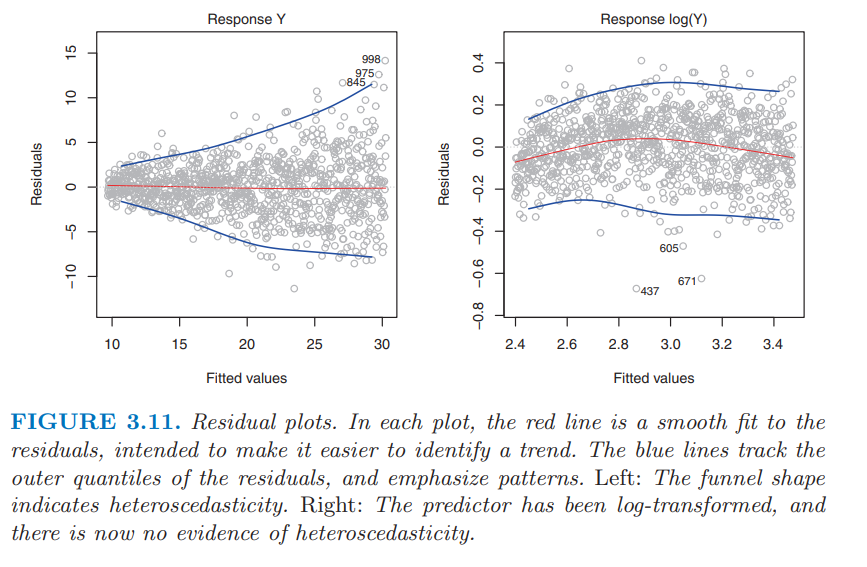
\includegraphics[scale=0.8]{images/non-const-var.png}
\end{center}
When faced with this problem, one possible solution is to transform the response $Y$ using a concave function such as $log \,\,Y$ or $\sqrt{Y}$ . Such a transformation results in a greater amount of shrinkage of the larger responses, leading to a reduction in heteroscedasticity.

\subsection{Outliers}
An outlier is a point for which $y_i$ is far from the value predicted by the model. Outliers can arise for a variety of reasons, such as incorrect recording of an observation during data collection.\\\\
 It is typical for an outlier that does not have an unusual
predictor value to have little effect on the least squares fit. However, even if an outlier does not have much effect on the least squares fit, it can cause other problems. For example, it can drastically affect the RSE or $R^2$ statistics. Since the RSE is used to compute all confidence intervals and p-values, such a dramatic increase caused by a single data point can have implications for the interpretation of the fit. If we believe that an outlier has occurred due to an error in data collection or recording, then one solution is to simply remove the observation. However, care should be taken, since an outlier may instead indicate a deficiency with the model, such as a missing predictor.

\subsection{High Leverage Points}
We just saw that outliers are observations for which the response $y_i$ is unusual given the predictor $x_i$. In contrast, observations with high leverage have an unusual value for $x_i$.
\begin{center}
    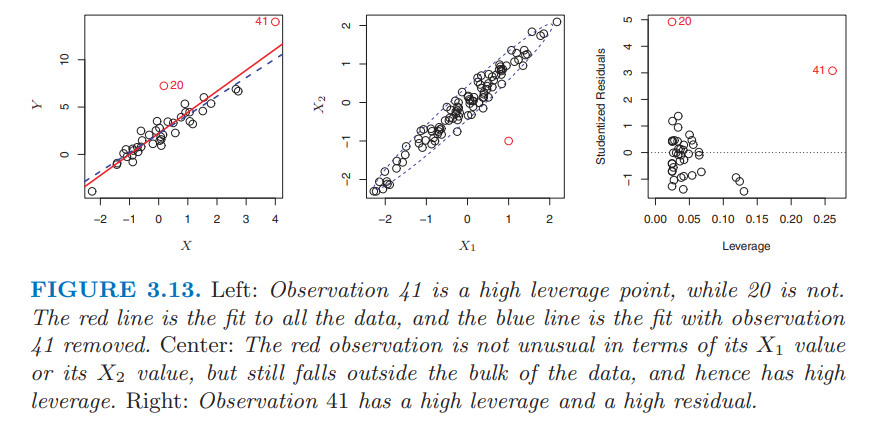
\includegraphics[scale=0.8]{images/high-laverage.png}
\end{center}
Removing the high leverage observation has a much more substantial impact on the least squares line than removing the outlier. In fact, high leverage observations tend to have a sizable impact on the estimated regression line. It is cause for concern if the least squares line is heavily affected by just a couple of observations,
because any problems with these points may invalidate the entire fit. For this reason, it is important to identify high leverage observations.

\subsection{Collinearity}
Collinearity refers to the situation in which two or more predictor variables are closely related to one another. The presence of collinearity can pose problems in the regression context, since it can be difficult to separate out the individual effects of collinear variables on the response.\\\\
Since collinearity reduces the accuracy of the estimates of the regression coefficients, it causes the standard error for $\hat\beta_j$ to grow. Recall that the t-statistic for each predictor is calculated by dividing $\hat\beta_j$ by its standard error. Consequently, collinearity results in a decline in the t-statistic. As a result, in the presence of collinearity, we may fail to reject $H0 : \beta_j = 0$.\\\\
A simple way to detect collinearity is to look at the correlation matrix of the predictors. An element of this matrix that is large in absolute value indicates a pair of highly correlated variables, and therefore a collinearity problem in the data. Unfortunately, not all collinearity problems can be detected by inspection of the correlation matrix: it is possible for collinearity to exist between three or more variables even if no pair of variables has a particularly high correlation. We call this situation \textit{multicollinearity}.

\chapter{Lec 09 - Linear Regression III}

\section{Comparison of Linear Regression with K-Nearest Neighbors}
Linear regression is an example of a parametric approach because it assumes a linear functional form for $f(X)$.  Parametric methods have several advantages. They are often easy to fit, because one need estimate only a small number of coefficients.  But parametric methods do have a disadvantage: by construction, they make strong assumptions about the form of $f(X)$. If the specified functional form is far from the truth, and prediction accuracy is our goal, then the parametric method will perform poorly.\\\\
In contrast, non-parametric methods do not explicitly assume a parametric form for $f(X)$, and thereby provide an alternative and more flexible approach for performing regression. Here we consider one of the simplest and best-known
non-parametric methods, \textit{K-nearest neighbors} regression (KNN regression).\\\\
Given a value for $K$ and a prediction point $x_0$, KNN regression first identifies the $K$ training observations that are closest to $x_0$, represented by $\mathcal{N}_0$. It then estimates $f(x_0)$ using the average of all the training responses in $\mathcal{N}_0$. In other words,
\[\hat{f}(x_0) = \frac{1}{K}\sum_{x_i \in \mathcal{N}_0} y_i\]
In general, the optimal value for $K$ will depend on the bias-variance tradeoff. A small value for $K$ provides the most flexible fit, which will
have low bias but high variance. This variance is due to the fact that the
prediction in a given region is entirely dependent on just one observation.
In contrast, larger values of $K$ provide a smoother and less variable fit; the
prediction in a region is an average of several points, and so changing one observation has a smaller effect. However, the smoothing may cause bias by masking some of the structure in $f(X)$.
\begin{center}
    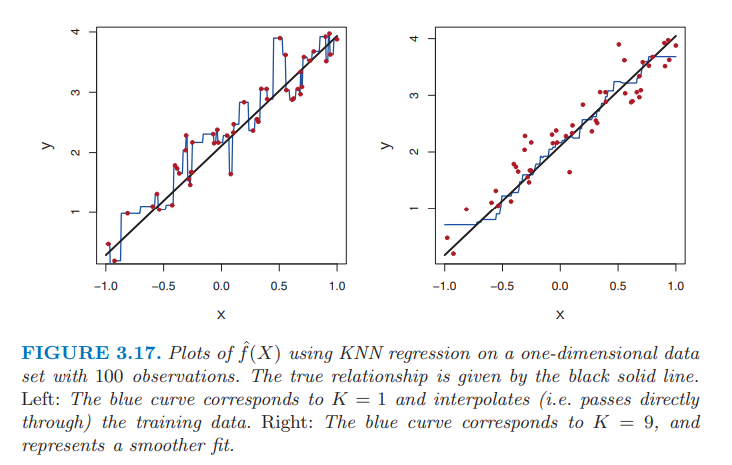
\includegraphics[scale=0.8]{images/linear-reg vs knn.png}
    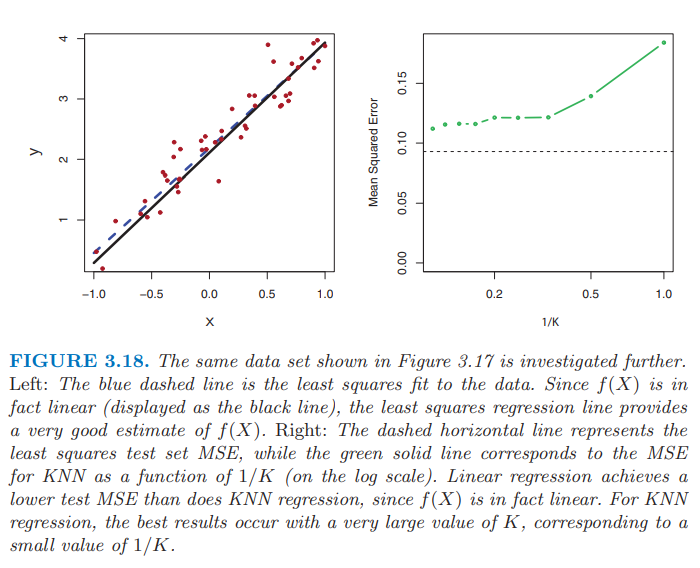
\includegraphics[scale=0.8]{images/knn.png}
\end{center}
The figures above provide an example with data generated from a one-dimensional linear regression model. The black solid lines represent $f(X)$, while the blue curves correspond to the KNN fits using $K = 1$ and $K = 9$. In this case, the $K = 1$ predictions are far too variable, while
the smoother $K = 9$ fit is much closer to $f(X)$. However, since the true
relationship is linear, it is hard for a non-parametric approach to compete with linear regression.
\begin{center}
    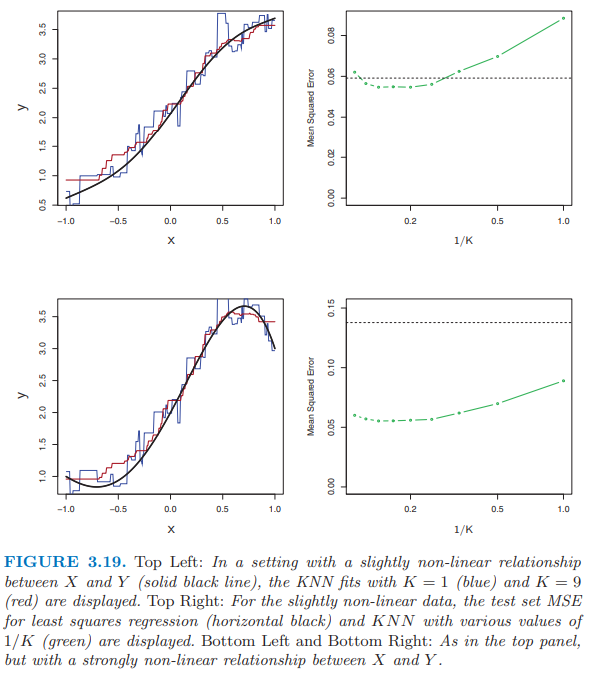
\includegraphics[scale=0.8]{images/linear-reg vs knn 2.png}
\end{center}
The figure above examines the relative performances of least squares regression and KNN under increasing levels of non-linearity in the relationship
between $X$ and $Y$ . In the top row, the true relationship is nearly linear.
In this case we see that the test MSE for linear regression is still superior
to that of KNN for low values of $K$. However, for $K \geq 4$, KNN outperforms linear regression. The second row illustrates a more substantial deviation from linearity. In this situation, KNN substantially outperforms linear regression for all values of $K$.\\\\
When $p = 1$ or $p = 2$, KNN outperforms linear regression. But for $p = 3$ the results are mixed, and for $p \geq 4$ linear regression is superior to KNN. This is caused by the curse of dimensionality that we already discussed.
\begin{center}
    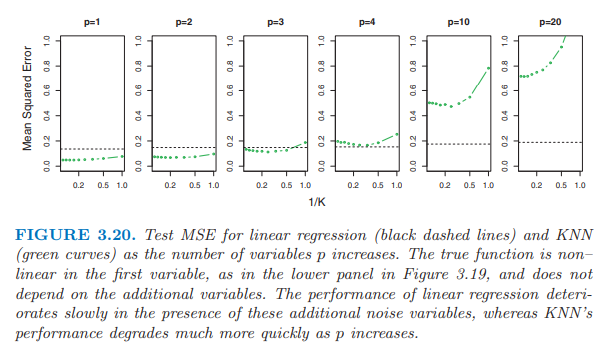
\includegraphics[scale=0.8]{images/curse of dim.png}
\end{center}
Even in problems in which the dimension is small, we might prefer linear regression to KNN from an interpretability standpoint.

\chapter{Lec 10 - Intro to Classification \& Model Selection}

\maketitle

\section{The Classification Setting}
Suppose that we seek to estimate $f$ on the basis of training observations $\{(x_1, y_1), ..., (x_n, y_n)\}$, where now $y_1,...,y_n$ are qualitative. The most common approach for quantifying the accuracy of our estimate $\hat{f}$ is the training error rate, the proportion of mistakes that are made if we apply our estimate $\hat{f}$ to the training observations:
\begin{equation}
    \frac{1}{n} \sum_{i=1}^n I(y_i \neq \hat{y}_i)
    \label{accuracy}
\end{equation}
Here $\hat{y}_i$ is the predicted class label for the $i$-th observation using $\hat{f}$. And $I(y_i \neq \hat{y}_i)$ is an indicator variable that equals 1 if $y_i \neq \hat{y}_i$ and zero if $y_i = \hat{y}_i$. Hence Equation \ref{accuracy} computes the fraction of incorrect classifications.\\\\
As in the regression setting, we are most interested in the error rates that result from applying our classifier to test observations that were not used in training. The \textit{test error} rate associated with a set of test observations of the form $(x_0, y_0)$ is given by
\begin{equation}
    Ave(I(y_0 \neq \hat{y}_0))
    \label{test-accuracy}
\end{equation}
A good classifier is one for which the test error \ref{test-accuracy} is smallest. It is possible to show that the test error rate given in \ref{test-accuracy} is minimized, on average, by a very simple classifier that assigns each observation to the most likely class, given its predictor values.  In other words, we should simply assign a test observation with predictor vector $x_0$ to the class $j$ for which
\begin{equation}
    P(Y=j | X=x_0)
    \label{cond prob}
\end{equation}
is largest. Note that \ref{cond prob} is a conditional probability: it is the probability that $Y = j$, given the observed predictor vector $x_0$. This very simple classifier is called the \textbf{Bayes classifier}. The Bayes classifier produces the lowest possible test error rate, called the \textit{Bayes error rate}.
\paragraph{K-Nearest Neighbors:} 
In theory we would always like to predict qualitative responses using the Bayes classifier. But for real data, we do not know the conditional distribution of $Y$ given $X$, and so computing the Bayes classifier is impossible. Therefore, the Bayes classifier serves as an unattainable gold standard against which to compare other methods. Many approaches attempt to estimate the conditional distribution of $Y$ given $X$, and then classify a given observation to the class with highest estimated probability.\\\\
One such method is the K-nearest neighbors (KNN) classifier. Given a positive integer $K$ and a test observation $x_0$, the KNN classifier first identifies the $K$ points in the training data that are closest to $x_0$, represented by $\mathcal{N}_0$. It then estimates the conditional probability for class $j$ as the fraction of points in $\mathcal{N}_0$ whose response values equal $j$:
\begin{equation}
    P(Y = j | X = x_0) = \frac{1}{K} \sum_{i \in \mathcal{N}_0} I(y_i = j)
\end{equation}
Finally, KNN applies Bayes rule and classifies the test observation $x_0$ to the class with the largest probability.
\begin{center}
    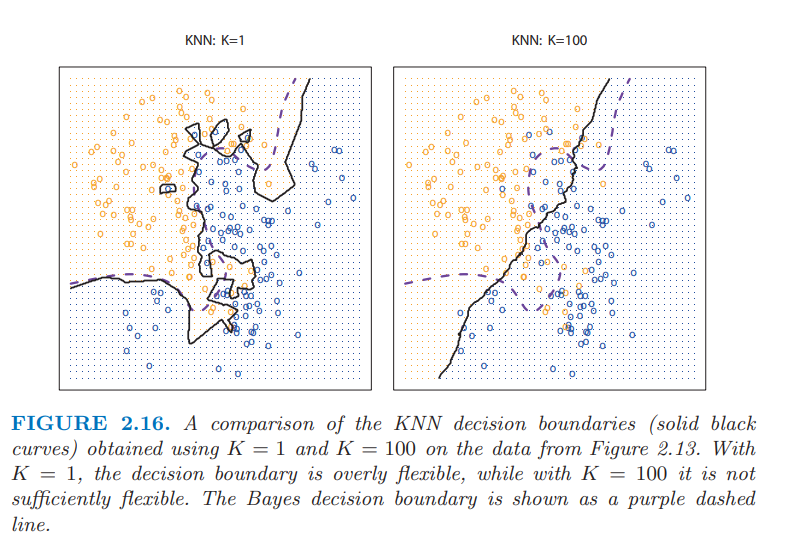
\includegraphics[scale=0.8]{images/knn-classification.png}
\end{center}
The choice of $K$ has a drastic effect on the KNN classifier obtained. When $K = 1$, the decision boundary is overly flexible and finds patterns in the data that don’t correspond to the Bayes decision boundary. This corresponds to a classifier that has low bias but very high variance. As $K$ grows, the method becomes less flexible and produces a decision boundary that is close to linear. This corresponds to a low-variance but high-bias classifier.
\begin{center}
    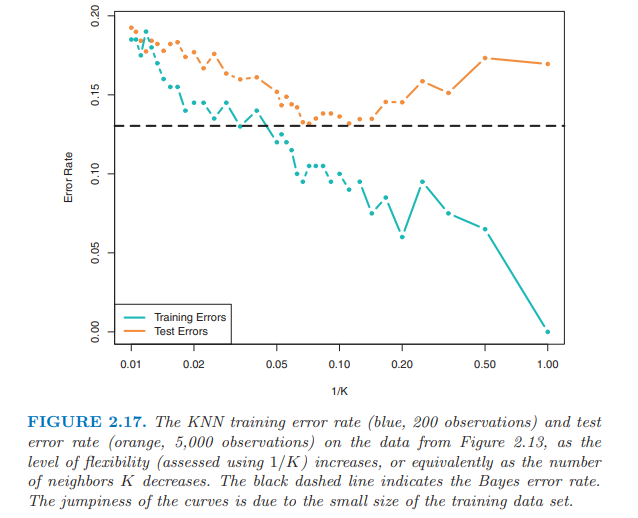
\includegraphics[scale=0.7]{images/knn-training-val error.png}
\end{center}
In Figure above, we have plotted the KNN test and training errors as a function of $1/K$. As $1/K$ increases, the method becomes more flexible. As in the regression setting, the training error rate consistently declines as the flexibility increases. However, the test error exhibits a characteristic U-shape, declining at first (with a
minimum at approximately$ K = 10$) before increasing again when the
method becomes excessively flexible and overfits.

\section{Cross-Validation}
In the absence of a very large designated test set that can be used to
directly estimate the test error rate, a number of techniques can be used to estimate this quantity using the available training data. Here we consider a class of methods that estimate the test error rate by holding out a subset of the training observations from the fitting process, and then applying the statistical learning method to those held out observations.

\subsection{The Validation Set Approach}
Suppose that we would like to estimate the test error associated with fitting a particular statistical learning method on a set of observations. The \textbf{validation set} approach is a very simple strategy for this task.  It involves randomly dividing the available set of observations into two parts, a training set and a \textit{validation set} or \textit{hold-out set}. The model is fit on the training set, and the fitted model is used to predict the responses for the observations in the validation set. The resulting validation set error rate—typically assessed using MSE in the case of a quantitative response—provides an estimate of the test error rate.
\begin{center}
    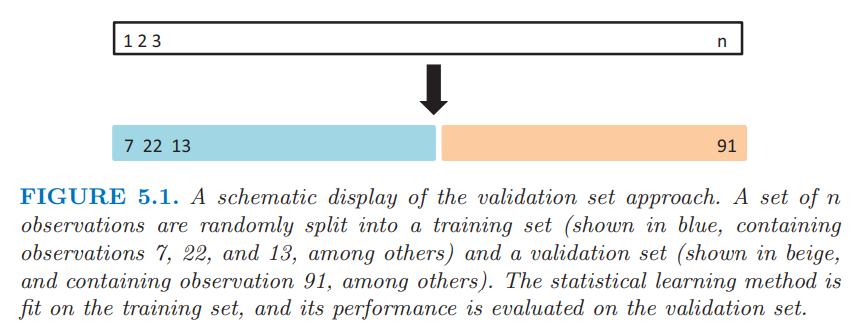
\includegraphics[scale=0.8]{images/cv.png}
\end{center}
The validation set approach is conceptually simple and is easy to implement. But it has two potential drawbacks:
\begin{enumerate}
    \item The validation estimate of the test error rate can be highly variable, depending on precisely which observations are included in the training set and which observations are included in the validation set.

    \item  In the validation approach, only a subset of the observations—those that are included in the training set rather than in the validation set—are used to fit the model. Since statistical methods tend to perform worse when trained on fewer observations, this suggests that the validation set error rate may tend to overestimate the test error rate for the model fit on the entire data set.

\end{enumerate}

\begin{center}
    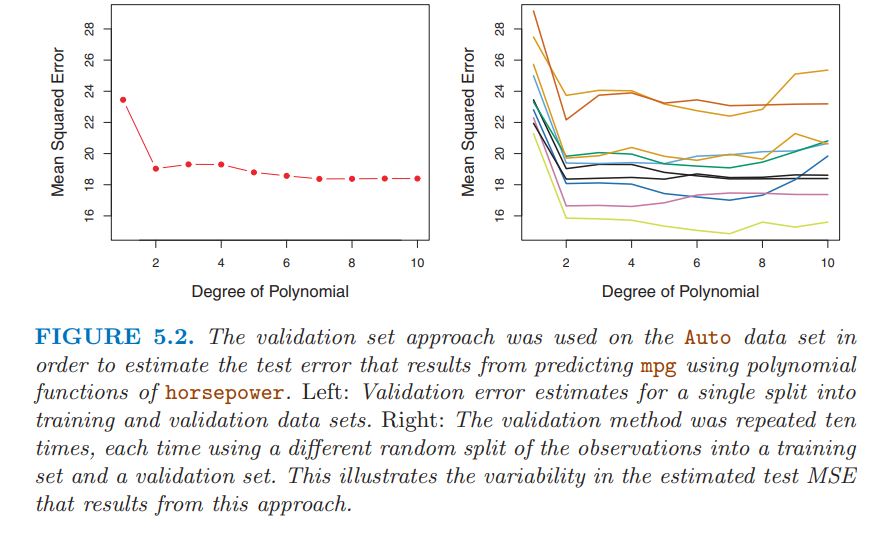
\includegraphics[scale=0.7]{images/cv2.png}
\end{center}
In the coming subsections, we will present \textit{cross-validation}, a refinement of the validation set approach that addresses these two issues.

\subsection{\textit{k}-Fold Cross-Validation}
This approach involves randomly dividing the set of observations into $k$ groups, or folds, of approximately equal size. The first fold is treated as a validation set, and the model is fit on the remaining $k - 1$ folds. The mean squared error, $MSE_1$, is then computed on the observations in the held-out fold. This procedure is repeated $k$ times; each time, a different group of observations is treated as a validation set. This process results in $k$ estimates of the test error, $MSE_1, MSE_2,..., MSE_k$. The $k$-fold CV estimate is computed by averaging these values
\begin{equation}
    CV_{(k)} = \frac{1}{k} \sum_{i=1}^k MSE_i
\end{equation}

\begin{center}
    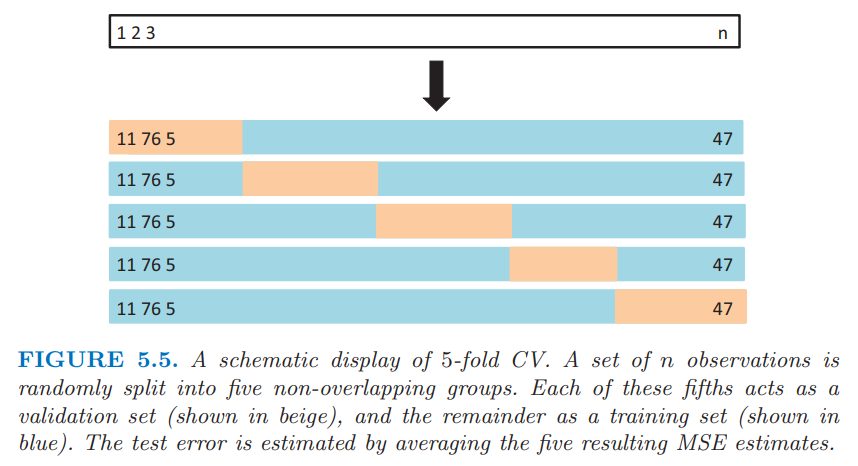
\includegraphics[scale=0.7]{images/k-fold-cv.png}
\end{center}
If we set $k=n$, we'll have $n$ folds or \textit{leave one out cross validation} (LOOCV).  In practice, one typically performs $k$-fold CV using $k = 5$ or $k = 10$. What is the advantage of using $k = 5$ or $k = 10$ rather than $k = n$? The most obvious advantage is computational. LOOCV requires fitting the statistical learning method $n$ times. This has the potential to be computationally expensive.  Putting computational issues aside, a less obvious but potentially more important advantage of $k$-fold CV is that it often gives more accurate estimates of the test error rate than does LOOCV. This has to do with a bias-variance trade-off.\\\\
Previously, we mentioned that the validation set approach can
lead to overestimates of the test error rate, since in this approach the training set used to fit the statistical learning method contains only half the observations of the entire data set. Using this logic, it is not hard to see that LOOCV will give approximately unbiased estimates of the test error, since each training set contains $n - 1$ observations, which is almost as many as the number of observations in the full data set.\\\\
However, we know that bias is not the only source for concern in an estimating procedure; we must also consider the procedure’s variance. It turns out that LOOCV has higher variance than does $k$-fold CV with $k<n$. Why is this the case? When we perform LOOCV, we are in effect averaging the outputs of $n$ fitted models, each of which is trained on an almost identical set of observations; therefore, these outputs are highly (positively) correlated with each other. Since the mean of many highly correlated quantities has higher variance than does the mean of many quantities that are not as highly correlated, the test error estimate resulting from LOOCV tends to have higher variance than does the test error estimate resulting from $k$-fold CV.\\\\
To summarize, there is a bias-variance trade-off associated with the
choice of $k$ in $k$-fold cross-validation. Typically, given these considerations, one performs $k$-fold cross-validation using $k = 5$ or $k = 10$, as these values have been shown empirically to yield test error rate estimates that suffer neither from excessively high bias nor from very high variance.\\\\
When we perform cross-validation, our goal might be to determine how
well a given statistical learning procedure can be expected to perform on independent data; in this case, the actual estimate of the test MSE is of interest. But at other times we are interested only in the location of the minimum point in the estimated test MSE curve. This is because we might be performing cross-validation on a number of statistical learning methods, or on a single method using different levels of flexibility, in order to identify the method that results in the lowest test error.
\begin{center}
    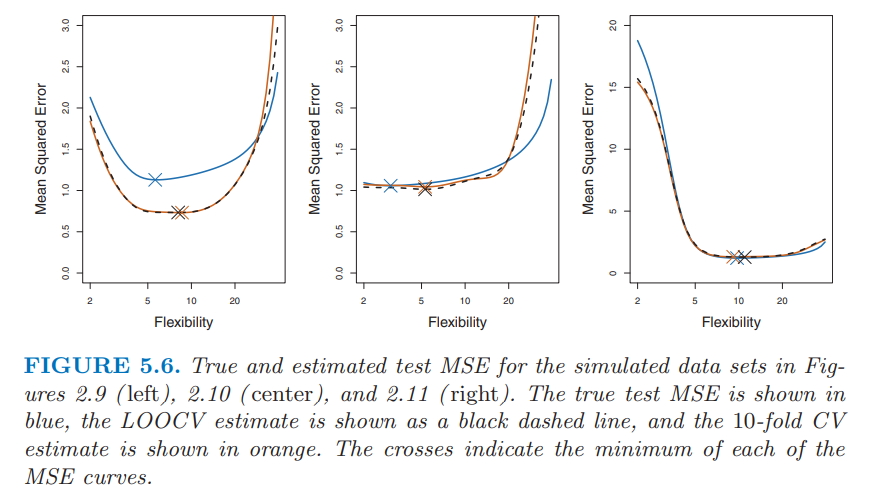
\includegraphics[scale=0.7]{images/k-fold-cv2.png}
\end{center}

\subsubsection{Data Leakage}
One common mistake which arises when performing $k$-fold cross validation is the so called \textit{data leakage} problem. In the context of $k$-fold cross validation, a common mistake is to perform data preparation on the entire dataset \textit{before} performing the cross validation procedure. Although this is a common approach, it is dangerously incorrect in most cases. 
\\\\
The problem with applying data preparation techniques before splitting data for model evaluation is that it can lead to data leakage and, in turn, will likely result in an incorrect estimate of a model’s performance.\\\\
Data leakage refers to a problem where information about the holdout dataset, such as a test or validation dataset, is made available to the model in the training dataset. This leakage is often small and subtle but can have a marked effect on performance.\\\\
The solution is straightforward: data preparation must be fit only on the training set inside the $k$-fold cross validation loop. That is, any coefficients or models prepared for the data preparation process must only use rows of data in the training dataset. Once fit, the data preparation algorithms or models can then be applied to the training set, and to the test set. This might include data transforms, but also other techniques such feature selection, dimensionality reduction, feature engineering and more. 

\chapter{Lec 11 - Model Selection II}

\maketitle

\section{Subset Selection}
In this section we consider some methods for selecting subsets of predictors. To perform best subset selection, we fit a separate least squares regression for each possible combination of the $p$ predictors. That is, we fit all $p$ models selection that contain exactly one predictor, all $p(p-1)/2$ models that contain
exactly two predictors, and so forth. We then look at all of the resulting models, with the goal of identifying the one that is best.\\\\
The problem of selecting the best model from among the $2^p$ possibilities
considered by best subset selection is not trivial. This is usually broken up
into two stages
\begin{center}
    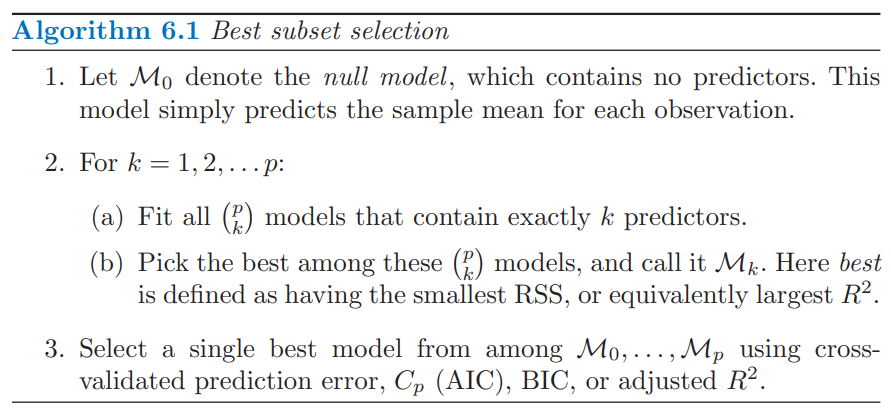
\includegraphics[scale=0.7]{images/best-subset.png}
\end{center}
In the algorithm above, Step 2 identifies the best model (on the training data)
for each subset size, in order to reduce the problem from one of $2^p$ possible models to one of $p + 1$ possible models. Now in order to select a single best model, we must simply choose among these $p + 1$ options. This task must be performed with care, because the RSS of these $p + 1$ models decreases monotonically, and the $R^2$ increases monotonically, as the number of features included in the models increases.\\\\
Therefore, if we use these statistics to select the best model, then we will
always end up with a model involving all of the variables. The problem is
that a low RSS or a high $R^2$ indicates a model with a low \textit{training error}, whereas we wish to choose a model that has a low \textit{test error}.
\\\\
Therefore, in Step 3, we use cross-validated prediction error, in order to select among $\mathcal{M}_0, \mathcal{M}_1, ..., \mathcal{M}_p$. While best subset selection is a simple and conceptually appealing approach, it suffers from computational limitations. The number of possible models that must be considered grows rapidly as $p$ increases.

\subsection{Stepwise Selection}
For computational reasons, best subset selection cannot be applied with
very large $p$. Best subset selection may also suffer from statistical problems when $p$ is large. The larger the search space, the higher the chance of finding models that look good on the training data, even though they might not have any predictive power on future data. Thus an enormous search space can lead to overfitting and high variance of the coefficient estimates. For both of these reasons, stepwise methods, which explore a far more restricted set of models, are attractive alternatives to best subset selection.
\paragraph{Forward Stepwise Selection.} Forward stepwise selection is a computationally efficient alternative to best subset selection. While the best subset selection procedure considers all $2^p$ possible models containing subsets of the $p$ predictors, forward stepwise considers a much smaller set of models. Forward stepwise selection begins with a model containing no predictors, and then adds predictors to the model, one-at-a-time, until all of the predictors are in the model. In particular, at each step the variable that gives the greatest \textit{additional} improvement to the fit is added to the model. More formally, the forward stepwise selection procedure is given in the following algorithm:
\begin{center}
    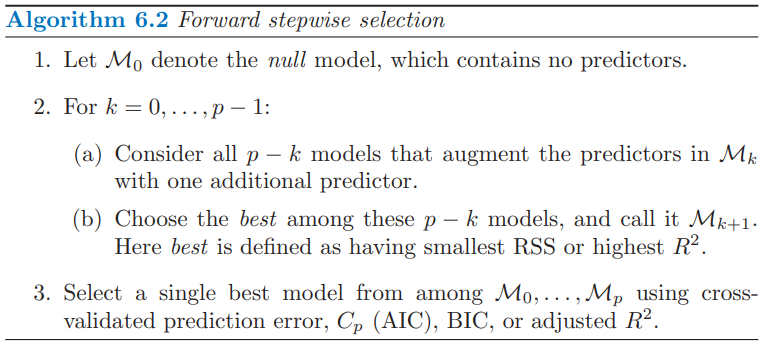
\includegraphics[scale=0.7]{images/forward stepwise.png}
\end{center}
Unlike best subset selection, which involved fitting $2^p$ models, forward
stepwise selection involves fitting one null model, along with $p - k$ models
in the $k$-th iteration, for $k = 0,...,p - 1$. This amounts to a total of $1 + \sum_{k=0}^{p-1} (p-k) = 1 + p(p+1)/2$ models.\\\\
In Step 2(b),  we must identify the best model from among those $p-k$ that augment $\mathcal{M}_k$ with one additional predictor. We can do this by simply choosing the model with the lowest RSS or the highest $R^2$. However, in Step 3, we must identify the best model among a set of models with different numbers of variables. This is more challenging, and
is discussed later.
\paragraph{Backward Stepwise Selection.} Like forward stepwise selection, backward stepwise selection provides an efficient alternative to best subset selection. However, unlike forward stepwise selection, it begins with the full least squares model containing all $p$ predictors, and then iteratively removes the least useful predictor, one-at-a-time.
\begin{center}
    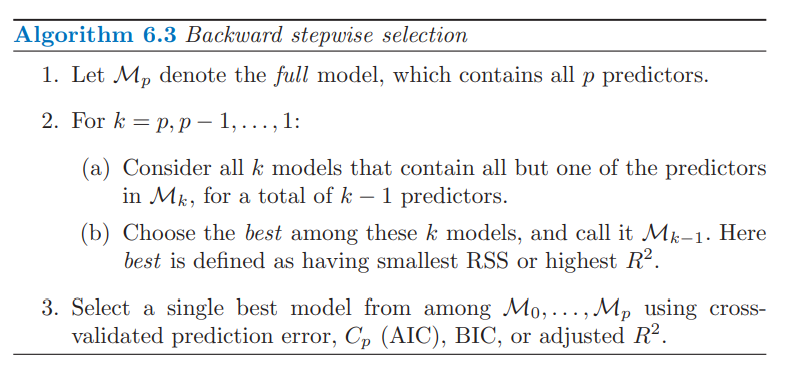
\includegraphics[scale=0.7]{images/backward stepwise.png}
\end{center}
Like forward stepwise selection, the backward selection approach searches
through only $1+p(p+ 1)/2$ models, and so can be applied in settings where
$p$ is too large to apply best subset selection. Also like forward stepwise
selection, backward stepwise selection is not guaranteed to yield the best
model containing a subset of the $p$ predictors.\\\\
Backward selection requires that the number of samples n is larger than
the number of variables $p$ (so that the full model can be fit). In contrast,
forward stepwise can be used even when $n<p$, and so is the only viable
subset method when $p$ is very large.
\paragraph{Hybrid Approaches.} The best subset, forward stepwise, and backward stepwise selection approaches generally give similar but not identical models. As another alternative, hybrid versions of forward and backward stepwise selection are available, in which variables are added to the model sequentially, in analogy to forward selection. However, after adding each new variable, the method may also remove any variables that no longer provide an improvement in the model fit. Such an approach attempts to more closely mimic best subset selection while retaining the computational advantages of forward and backward stepwise selection.

\subsection{Choosing the Optimal Model}
Best subset selection, forward selection, and backward selection result in the creation of a set of models, each of which contains a subset of the $p$ predictors. In order to implement these methods, we need a way to determine
which of these models is best. As we said previously, the model
containing all of the predictors will always have the smallest RSS and the
largest $R^2$, since these quantities are related to the training error. Instead, we wish to choose a model with a low test error.\\\\
In order to select the best model with respect to test error, we need to estimate this test error. There are two common approaches:
\begin{enumerate}
    \item We can indirectly estimate test error by making an adjustment to the training error to account for the bias due to overfitting.

    \item We can directly estimate the test error, using either a validation set approach or a cross-validation approach.
\end{enumerate}
MSE is generally an underestimate of the test MSE. (Recall that MSE = $RSS/n$.) This is because
when we fit a model to the training data using least squares, we specifically estimate the regression coefficients such that the training RSS (but not the test RSS) is as small as possible. Therefore, training set RSS and training set $R^2$ cannot be used to select from among a set of models with different numbers of variables.\\\\
However, a number of techniques for adjusting the training error for the model size are available. We now consider four such approaches: $C_p$, \textit{Akaike information criterion} (AIC), \textit{Bayesian information criterion} (BIC), and adjusted $R^2$.\\\\
For a fitted least squares model containing $d$ predictors, the $C_p$ estimate
of test MSE is computed using the equation
\[C_p = \frac{1}{n} (RSS + 2d \hat{\sigma}^2)\]
where $\hat{\sigma}^2$ is an estimate of the variance of the error  associated with each response measurement. Essentially, the $C_p$ statistic adds a penalty of $2d \hat{\sigma}^2$ to the training RSS in order to adjust for the fact that the training error tends to underestimate the test error. Clearly, the penalty increases as the number of predictors in the model increases; this is intended to adjust for the corresponding decrease in training RSS.\\\\
The AIC criterion is defined for a large class of models fit by maximum
likelihood. In the case of linear models with Gaussian errors, maximum
likelihood and least squares are the same thing. In this case AIC is given by
\[\text{AIC} = \frac{1}{n\hat{\sigma}^2}(\text{RSS} + 2d \hat{\sigma}^2)\]
where, for simplicity, we have omitted an additive constant.\\\\
BIC is derived from a Bayesian point of view, but ends up looking similar
to $C_p$ (and AIC) as well. For the least squares model with $d$ predictors, the BIC is, up to irrelevant constants, given by
\[\text{BIC} = \frac{1}{n} (\text{RSS} + log(n)d\hat{\sigma}^2)\]
Like $C_p$, the BIC will tend to take on a small value for a model with a
low test error, and so generally we select the model that has the lowest
BIC value. Notice that BIC replaces the $2d \hat{\sigma}^2$ used by $C_p$ with a $log(n)d\hat{\sigma}^2$ term, where $n$ is the number of observations. Since $log\, n > 2$ for any $n > 7$, the BIC statistic generally places a heavier penalty on models with many variables, and hence results in the selection of smaller models than $C_p$.\\\\
The adjusted $R^2$ statistic is another popular approach for selecting among
a set of models that contain different numbers of variables. For a least squares model with $d$ variables, the adjusted $R^2$ statistic is calculated as
\[\text{Adjusted } R^2 = 1 - \frac{\text{RSS} / (n - d - 1)}{\text{TSS}/(n-1)}\]
Unlike $C_p$, AIC, and BIC, for which a small value indicates a model with
a low test error, a large value of adjusted $R^2$ indicates a model with a
small test error. Maximizing the adjusted $R^2$ is equivalent to minimizing
$\frac{RSS}{n - d - 1}$. The intuition behind the adjusted $R^2$ is that once all of the correct variables have been included in the model, adding additional noise variables will lead to only a very small decrease in RSS. Since adding noise variables leads to an increase in d, such variables will lead to an increase in $\frac{RSS}{n - d - 1}$, and consequently a decrease in the adjusted $R^2$. Therefore, in theory, the model with the largest adjusted $R^2$ will have only correct variables and no noise variables.
\paragraph{Validation and Cross-Validation} 
As an alternative to the approaches just discussed, we can directly estimate the test error using the validation set and cross-validation methods. We can compute the validation set error or the cross-validation error for each model under consideration, and then select the model for which the resulting estimated test error is smallest. This procedure has an advantage relative to AIC, BIC, $C_p$, and adjusted $R_2$, in that it provides a direct estimate of the test error, and makes fewer assumptions about the true underlying model. It can also be used in a wider range of model selection tasks, even in cases where it is hard to pinpoint the model degrees of freedom (e.g. the number of predictors in the model) or hard to estimate the error variance $\sigma^2$. However, cross-validation is computationally heavier than the previous methods.

\section{Principal Components Regression}
The principal components regression (PCR) approach involves constructing the first $M$ principal components, $Z_1,...,Z_M$, and then using these components as the predictors in a linear regression model that is fit using least squares. The key idea is that often a small number of principal components suffice to explain most of the variability in the data, as well as the relationship with the response. In other words, we assume that the directions in which $X_1,...,X_p$ show the most variation are the directions that are associated with $Y$.\\\\
While this assumption is not guaranteed to be true, it often turns out to be a reasonable enough approximation to give good results. If the assumption underlying PCR holds, then fitting a least squares model to $Z_1,...,Z_M$ will lead to better results than fitting a least squares model to $X_1,...,X_p$, since most or all of the information in the data that relates to the response is contained in $Z_1,...,Z_M$, and by estimating only $M << p$ coefficients we can mitigate overfitting.\\\\
We note that even though PCR provides a simple way to perform regression using $M<p$ predictors, it is \textit{not} a feature selection method. This is because each of the $M$ principal components used in the regression is a linear combination of all $p$ of the original features. In PCR, the number of principal components, $M$, is typically chosen by cross-validation.

\chapter{Lec TBL - Classification}

\section{Classification}
The linear regression model discussed before assumes that the response variable $Y$ is quantitative. But in many situations, the response variable is instead qualitative. For example, eye color is qualitative, taking on values blue, brown, or green. Often qualitative variables are referred to as categorical; we will use these terms interchangeably. In this chapter, we study approaches for predicting qualitative responses, a process that is known as classification.\\\\
Classification problems occur often, perhaps even more so than regression
problems. Some examples include:
\begin{itemize}
    \item A person arrives at the emergency room with a set of symptoms
    that could possibly be attributed to one of three medical conditions.
    Which of the three conditions does the individual have?

    \item An online banking service must be able to determine whether or not
    a transaction being performed on the site is fraudulent, on the basis
    of the user’s IP address, past transaction history, and so forth.

    \item On the basis of DNA sequence data for a number of patients with
    and without a given disease, a biologist would like to figure out which
    DNA mutations are deleterious (disease-causing) and which are not.
    
\end{itemize}
Just as in the regression setting, in the classification setting we have a
set of training observations $(x_1, y_1),...,(x_n, y_n)$ that we can use to build
a classifier. We want our classifier to perform well not only on the training
data, but also on test observations that were not used to train the classifier.

\section{Why Not Linear Regression?}
\label{lin_reg}
We have stated that linear regression is not appropriate in the case of a
qualitative response. Why not? Suppose that we are trying to predict the medical condition of a patient in the emergency room on the basis of her symptoms. In this simplified example, there are three possible diagnoses: \textit{stroke}, \textit{drug overdose}, and \textit{epileptic seizure}. We could consider encoding these values as a quantitative response variable, $Y$, as follows:
\[
Y = \begin{cases}
    1 & \text{if $stroke$}\\
    2 & \text{if \textit{drug overdose}}\\
    3 & \text{if \textit{epileptic seizure}}
\end{cases}
\]
Using this coding, least squares could be used to fit a linear regression model
to predict Y on the basis of a set of predictors $X_1,...,X_p$. Unfortunately, this coding implies an ordering on the outcomes, putting \textit{drug overdose} in between \textit{stroke} and \textit{epileptic seizure}, and insisting that the difference between \textit{stroke} and \textit{drug overdose} is the same as the difference between \textit{drug overdose} and \textit{epileptic seizure}.\\\\
For a binary (two level) qualitative response, the situation is better. For
instance, perhaps there are only two possibilities for the patient’s medical condition: \textit{stroke} and \textit{drug overdose}. We could then potentially use the dummy variable approach to code the response as follows:
\[
Y = \begin{cases}
    0 & \text{if $stroke$}\\
    1 & \text{if \textit{drug overdose}}
\end{cases}
\]
We could then fit a linear regression to this binary response, and predict
\textit{drug overdose} if $\hat{Y} > 0.5$ and \textit{stroke} otherwise. However, if we use linear regression, some of our estimates might be outside the $[0, 1]$ interval, making them hard to interpret as probabilities! The dummy variable approach cannot be easily extended to accommodate qualitative responses with more than two levels. For these
reasons, it is preferable to use a classification method that is truly suited for qualitative response values, such as the ones presented next.

\section{Logistic Regression}
Consider the Default data set, where the response default falls into
one of two categories, Yes or No. Rather than modeling this response $Y$
directly, logistic regression models the probability that $Y$ belongs to a particular category.
\[P(default = Yes | balance)\]
\begin{center}
    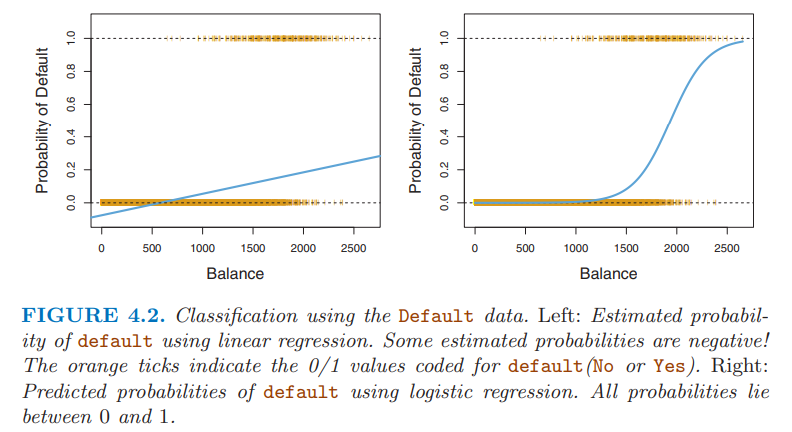
\includegraphics[scale=0.8]{images/logistic_reg.png}
\end{center}
The values of $P(default = Yes|balance)$, which we abbreviate $p(balance)$, will range between 0 and 1. One might predict $default = Yes$ for any individual for whom $p(balance) > 0.5$.\\\\
How should we model the relationship between $p(X) = P(Y = 1|X)$ and $X$? In section \ref{lin_reg} we talked of using a linear regression model to represent
these probabilities:
\[p(X) = \beta_0 + \beta_1X\]
If we use this approach to predict $default=Yes$ using $balance$, for balances close to zero we predict a negative probability of default. To avoid this problem, we must model $p(X)$ using a function that gives outputs between 0 and 1 for all values of $X$. Many functions meet this description. In logistic regression, we use the \textit{logistic function}:
\begin{equation}
    p(X) = \frac{e^{\beta_0 + \beta_1X}}{1 + e^{\beta_0 + \beta_1X}}
    \label{log_reg}
\end{equation}
To fit the model \ref{log_reg}, we use a method called maximum likelihood, which we discuss in the next section. The logistic function will always produce
an \textit{S-shaped} curve, and so regardless of the value of $X$, we will obtain a sensible prediction. After a bit of manipulation of \ref{log_reg}, we find that
\begin{equation}
    \frac{p(X)}{1 - p(X)} = e^{\beta_0 + \beta_1X}
    \label{odds}
\end{equation}
The quantity $p(X)/[1-p(X)]$ is called \textit{the odds}. Values of the odds close to 0 and $\infty$ indicate very low and very high probabilities of default, respectively. For example, on average 1 in 5 people with an odds of 1/4 will default, since p$(X)=0.2$ implies an odds of $\frac{0.2}{1 - 0.2} = 1/4$. By taking the logarithm of both sides of $\ref{odds}$, we arrive at:
\[log\left(\frac{p(X)}{1 - p(X)}\right) = \beta_0 + \beta_1X\]
The left-hand side is called the \textit{log-odds} or \textit{logit}. In a linear regression model, $\beta_1$ gives the average change in $Y$ associated with a one-unit increase in $X$. In contrast, in a logistic regression model, increasing $X$ by one unit changes the log odds by $\beta_1$. However, because the relationship between $p(X)$ and $X$ in \ref{log_reg} is not a straight line, $\beta_1$ does not correspond to the change in $p(X)$ associated with a one-unit increase in $X$. The amount that $p(X)$ changes due to a one-unit change in $X$ will depend on the current value of $X$. But regardless of the value of $X$, if $\beta_1$ is positive then increasing $X$ will be associated with increasing $p(X)$, and if $\beta_1$ is negative then increasing $X$ will be associated with decreasing $p(X)$.

\subsection{Estimating the Regression Coefficients}
The coefficients $\beta_0$ and $\beta_1$ in \ref{log_reg} are unknown, and must be estimated based on the available training data. Although we could use (non-linear) least squares, the more general method of maximum likelihood is preferred, since it has better statistical properties. The basic intuition behind using maximum likelihood
to fit a logistic regression model is as follows: we seek estimates for $\beta_0$ and
$\beta_1$ such that the predicted probability $\hat{p}(xi)$ of default for each individual, using \ref{log_reg}, corresponds as closely as possible to the individual’s observed default status. This intuition can be formalized using a mathematical equation called a \textit{likelihood function}:
\[l(\beta_0, \beta_1) = \prod_{i:y_i = 1} p(x_i) \prod_{i':y_{i'}=0} (1 - p(x_{i'}))\]
The estimates $\hat\beta_0$ and $\hat\beta_1$ are chosen to \textit{maximize} this likelihood function. In the linear regression setting, the least squares approach is in fact a special case of maximum likelihood. Once the coefficients have been estimated, it is a simple matter to compute the probability by plugging  $\hat\beta_0$ and $\hat\beta_1$ into \ref{log_reg}.

\subsection{Multiple Logistic Regression}
We now consider the problem of predicting a binary response using multiple predictors. By analogy with the extension from simple to multiple linear regression, we can generalize as follows:
\[log\left(\frac{p(X)}{1 - p(X)}\right) = \beta_0 + \beta_1 X_1 + ... + \beta_p X_p\]
Just as before, we use the maximum likelihood method to estimate the coefficients.

\subsection{Logistic Regression for $>2$ Response Classes}
We sometimes wish to classify a response variable that has more than two classes. The two-class logistic regression models discussed in the previous sections have multiple-class extensions, but in practice they tend not to be used all that often. One of the reasons is that the method we discuss in the next section, \textit{discriminant analysis}, is popular for multiple-class classification. So we do not go into the details of multiple-class logistic regression here.

\section{Linear Discriminant Analysis}
Logistic regression involves directly modeling $Pr(Y = k|X = x)$ using the logistic function. We now consider an alternative and less direct approach to estimating these probabilities. In this alternative approach, we model the distribution of the predictors $X$ separately in each of the response classes (i.e. given $Y$), and then use Bayes’ theorem to flip these around into estimates for $Pr(Y = k|X = x)$. Why do we need another method, when we have logistic regression? There are several reasons:
\begin{itemize}
    \item When the classes are well-separated, the parameter estimates for the logistic regression model are surprisingly unstable. Linear discriminant analysis does not suffer from this problem.

    \item If $n$ is small and the distribution of the predictors X is approximately normal in each of the classes, the linear discriminant model is again more stable than the logistic regression model.

    \item Linear discriminant analysis is popular when we have more than two response classes.
\end{itemize}

\subsection{Using Bayes’ Theorem for Classification}
Suppose that we wish to classify an observation into one of $K$ classes, where $K > 2$. Let $\pi_k$ represent the overall or prior probability that a randomly chosen observation comes from the $k$th class; Let $f_k(X) \equiv Pr(X = x|Y = k)$ denote the density function of $X$ for an observation that comes from the $k$th class. In other words, $f_k(x)$ is relatively large if there is a high probability that an observation in the $k$th class has $X \approx x$, and it is small otherwise. Then Bayes’
theorem states that \footnote{Note that the denominator serves to normalize the probability between 0 and 1}:
\begin{equation}
    Pr(Y = k|X = x) = \frac{\pi_k f_k(x)}{\sum_{l=1}^K \pi_l f_l(x)}
    \label{lda}
\end{equation}
In accordance with our earlier notation, we will use the abbreviation $p_k(X)
= Pr(Y = k|X)$. Then, we just need to estimate $\pi_k$ and $f_k(X)$ and plug them into \ref{lda} to make a prediction. In general, estimating $\pi_k$ is easy,  we simply compute the fraction of the training observations that belong to the $k$th class. However, estimating $f_k(X)$ tends to be more challenging, unless we assume some simple forms for these densities.\\\\
We know that the Bayes classifier, which classifies an observation to the class for which $p_k(X)$ is largest, has the lowest possible error rate out of all classifiers. If we can find a way to estimate $f_k(X)$, then we can develop a classifier that approximates the Bayes classifier.

\subsection{Linear Discriminant Analysis for $p = 1$}
For now, assume that p = 1, that is, we have only one predictor. We would like to obtain an estimate for $f_k(x)$ that we can plug into \ref{lda}. We will then classify an observation to the class for which $p_k(x)$ is greatest.\\\\
Suppose we assume that $f_k(x)$ is normal or Gaussian. In the one-dimensional setting, the normal density takes the form
\begin{equation}
    f_k(x) = \frac{1}{\sqrt{2\pi}\sigma_k}\text{exp}\left(-\frac{1}{2\sigma_k^2}(x - \mu_k)^2  \right)
    \label{normal_distr}
\end{equation}
where $\mu_k$ and $\sigma_k^2$ are the mean and variance parameters for the $k$th class. For now, let us further assume that $\sigma_1^2 = ... = \sigma_K^2$: that is, there is a shared variance term across all $K$ classes, which for simplicity we can denote by $\sigma^2$. Plugging \ref{normal_distr} into \ref{lda}, we find that
\begin{equation}
    p_k(x) = \frac{\pi_k \frac{1}{\sqrt{2\pi}\sigma}\text{exp}(-\frac{1}{2\sigma^2}(x - \mu_k)^2)}{\sum_{l=1}^K \pi_l \frac{1}{\sqrt{2\pi}\sigma}\text{exp}(-\frac{1}{2\sigma^2}(x - \mu_l)^2)}
    \label{lda_2}
\end{equation}
The Bayes classifier involves assigning an observation X = x to the class for which \ref{lda_2} is largest. Taking the log of \ref{lda_2} and rearranging the terms, it is not hard to show that this is equivalent to assigning the observation to the class for which
\begin{equation}
    \delta_k(x) = x \cdot \frac{\mu_k}{\sigma^2} - \frac{\mu_k^2}{2\sigma^2} + \text{log}(\pi_k)
    \label{discriminant}
\end{equation}
is largest.
\\\\
In practice, even if we are quite certain of our assumption that $X$ is drawn from a Gaussian distribution within each class, we still have to estimate the parameters $\mu_1,...,\mu_K, \pi_1,...,\pi_K$, and $\sigma^2$. The \textit{linear discriminant analysis} (LDA) method approximates the Bayes classifier by computing the following estimates
\[\begin{split}
    \hat{\mu}_k & = \frac{1}{n_k}\sum_{i:y_i = k}x_i\\
    \hat{\sigma}^2 & = \frac{1}{n - K}\sum_{k=1}^K\sum_{i:y_i = k} (x_i - \hat{\mu}_k)^2
\end{split}\] 
where $n$ is the total number of training observations, and $n_k$ is the number of training observations in the $k$th class. The estimate for $\mu_k$ is simply the average of all the training observations from the $k$th class, while $\hat{\sigma}^2$ can be seen as a weighted average of the sample variances for each of the $K$ classes. The LDA classifier plugs these estimates in \ref{discriminant} to make a prediction. The word linear in the classifier’s name stems from the fact that the \textit{discriminant functions} $\delta_k(x)$  are linear functions of $x$.

\subsection{Linear Discriminant Analysis for $p >1$}
We now extend the LDA classifier to the case of multiple predictors. To
do this, we will assume that $X = (X_1, X_2,...,X_p)$ is drawn from a multivariate Gaussian distribution with a class-specific mean vector and a common covariance matrix. The multivariate Gaussian distribution assumes that each individual predictor follows a one-dimensional normal distribution  with some correlation between each pair of predictors.\\\\
To indicate that a $p$-dimensional random variable $X$ has a multivariate Gaussian distribution, we write $X \sim N(\mu, \Sigma)$. Here $E(X) = \mu$ is the mean of $X$ (a vector with p components), and $Cov(X) = \Sigma$ is the $p \times p$ covariance matrix of $X$. 
In the case of $p > 1$ predictors, the LDA classifier assumes that the
observations in the $k$th class are drawn from a multivariate Gaussian distribution $N(\mu_k, \Sigma)$, where $\mu_k$ is a class-specific mean vector, and $\Sigma$ is a covariance matrix that is common to all $K$ classes. In particular $\mu_k$ is a $k$-dimensional vector with one value per class, while $\Sigma$ is a matrix which contains covariances between predictors.
\\\\
The density function $f_k(x)$, the discriminant function $\delta_k(x)$ and the subsequent prediction process are generalization of the ones presented before. Also the estimate of the parameters is done in a similar way as in the one-dimensional case.\\\\
We can perform LDA on the \textbf{Default} data in order to predict whether
or not an individual will default on the basis of credit card balance and student status. The LDA model fit to the 10, 000 training samples results
in a training error rate of 2.75\%. This sounds like a low error rate, but two caveats must be noted.
\begin{itemize}
    \item First of all, training error rates will usually be lower than test error rates, which are the real quantity of interest. The higher the ratio of parameters $p$ to number of samples $n$, the more we expect this overfitting to play a role.

    \item Second, since only 3.33\% of the individuals in the training sample defaulted, a simple but useless classifier that always predicts that each individual will not default, regardless of his or her credit card balance and student status, will result in an error rate of 3.33\%. In other words, the trivial null classifier will achieve an error rate that is only a bit higher than the LDA training set error rate.
\end{itemize}
In practice, a binary classifier such as this one can make two types of
errors: it can incorrectly assign an individual who defaults to the no default category, or it can incorrectly assign an individual who does not default to the default category. It is often of interest to determine which of these two types of errors are being made.
\begin{center}
    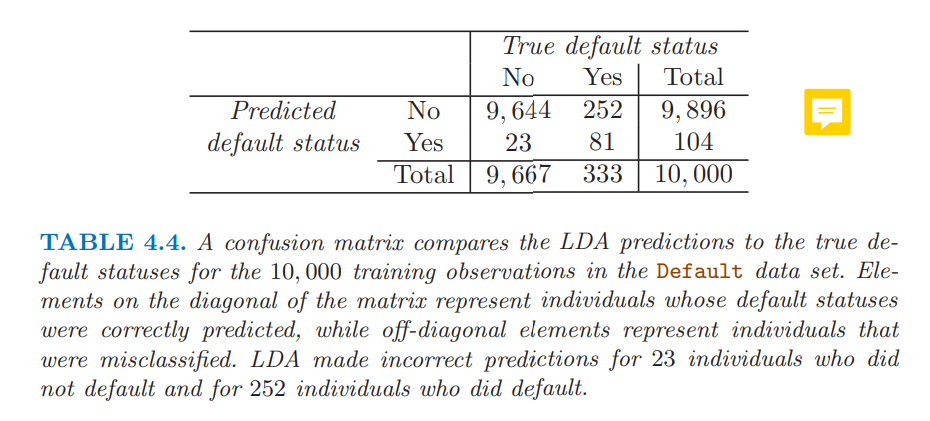
\includegraphics[scale=0.8]{images/confusion-matrix.png}
\end{center}
A \textit{confusion matrix}, shown in the Table above, is a convenient way to display this information. The table reveals that LDA predicted that a total of 104 people would default. Of these people, 81 actually defaulted and 23 did not. Hence only 23 out of 9, 667 of the individuals who did not default were incorrectly labeled. This looks like a pretty low error rate! However, of the 333 individuals who defaulted, 252 (or 75.7\%) were missed by LDA. So while the overall error rate is low, the error rate among individuals who defaulted is very high.\\\\
Class-specific performance is also important in medicine and biology,
where the terms \textit{sensitivity} and \textit{specificity} characterize the performance of a classifier or screening test. In this case the sensitivity is the percentage of true defaulters that are identified, a low 24.3\% in this case. The specificity is the percentage of non-defaulters that are correctly identified, here 9644/9667 = 99,8\%. More in general, the sensitivity is given by $TP/(TP + FN)$, where $TP$ and $FN$ stand for True Positive and False Negative, while the specificity is given by $TN/(TN + FP)$, where $TN$ and $FP$ stand for True Negative and False Positive. The accuracy is instead given by $(TP + TN) / Total = (9644 + 81) / 10000 = 97,25\%$. From the perspective of a credit card company that is trying to identify high-risk individuals, minimize the number of false negative is crucial.\\\\
Why does LDA do such a poor job of classifying the customers who default? As we have
seen, LDA is trying to approximate the Bayes classifier, which has the lowest total error rate out of all classifiers (if the Gaussian model is correct). That is, the Bayes classifier will yield the smallest possible total number of misclassified observations, irrespective of which class the errors come from. We will now see that it is possible to modify LDA in order to develop a classifier that better meets the credit card company’s needs.\\\\
The Bayes classifier works by assigning an observation to the class for which the posterior probability $p_k(X)$ is greatest. In the two-class case, the Bayes classifier, and by extension LDA, uses a threshold of 50\% for the posterior probability of default in order to assign an observation to the default class. However, if we are concerned about incorrectly predicting the default status for individuals who default, then we can consider
lowering this threshold. For instance, we might label any customer with a
posterior probability of default above 20\% to the default class.
\[Pr(default = Yes|X = x) > 0.2\]
With this modification, the classifier will have less false negative, but more false positive.\\\\
How can we decide which threshold value is best? Such a decision must be based on domain knowledge, such as detailed information about the costs associated with default. The \textit{ROC curve} is a popular graphic for simultaneously displaying the two types of errors for all possible thresholds. The overall performance of a classifier, summarized over all possible thresholds, is given by the area under the (ROC) curve (AUC). An ideal ROC curve will hug the top left corner, so the larger the AUC the better the classifier.
\begin{center}
    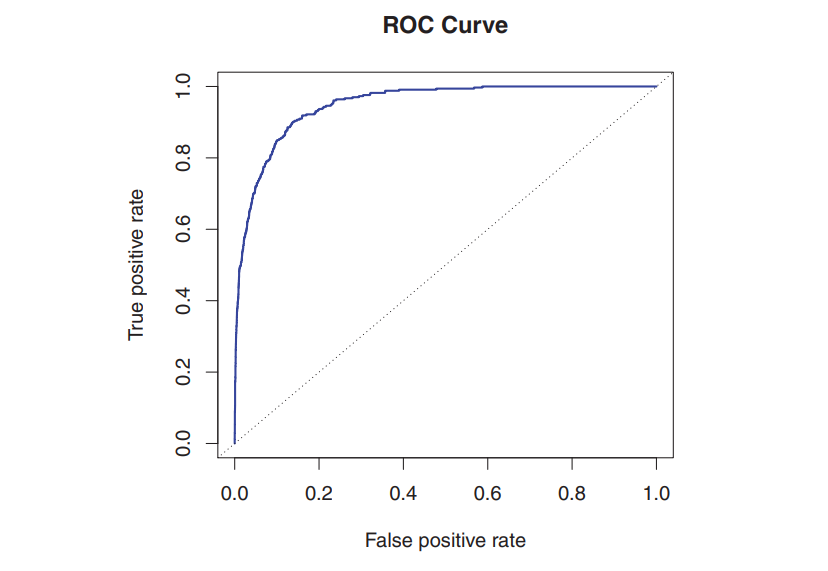
\includegraphics[scale=0.7]{images/ROC.png}
\end{center}
The Figure above shows A ROC curve for the LDA classifier on the Default data. It traces out two types of error as we vary the threshold value for the posterior probability of default. The actual thresholds are not shown. The true positive rate
is the sensitivity. The false positive rate is 1-specificity  The ideal ROC curve hugs the top left corner, indicating a high true positive rate and a low false positive rate. The dotted line represents the random classifier. The best threshold is the one associated with the value closest to the top-left corner. For more information about ROC curve visit the following post: \href{https://towardsdatascience.com/understanding-auc-roc-curve-68b2303cc9c5}{ROC CURVE}.

\section{Quadratic Discriminant Analysis}
As we have discussed, LDA assumes that the observations within each class are drawn from a multivariate Gaussian distribution with a class specific mean vector and a covariance matrix that is common to all K classes. Quadratic discriminant analysis (QDA) provides an alternative approach. Like LDA, the QDA classifier results from assuming that the observations from each class are drawn from a Gaussian distribution, and plugging estimates for the parameters into Bayes’ theorem in order to perform prediction. However, unlike LDA, QDA assumes that each class has its own covariance matrix. Unlike LDA, the quantity $x$ appears as a quadratic function in the discriminant function of QDA.\\\\
Why would one prefer LDA to QDA, or vice-versa? The answer lies in the bias-variance trade-off. When there are $p$ predictors, then estimating a covariance matrix requires estimating $p(p+1)/2$ parameters. QDA estimates a separate covariance matrix for each class, for a total of $Kp(p+1)/2$ parameters.  LDA is a much less flexible classifier than QDA, and so has substantially lower variance. This can potentially lead to improved prediction performance. But there is a trade-off: if LDA’s assumption that the $K$ classes share a common covariance matrix is badly off, then LDA can suffer from high bias. LDA tends to be a better bet than QDA if there are relatively few training observations and so reducing variance is crucial. In contrast, QDA is recommended if the training set is very large, so that the variance of the classifier is not a major concern, or if the assumption of a common covariance matrix for the $K$ classes is clearly untenable.

\section{A Comparison of Classification Methods}
Though their motivations differ, the logistic regression and LDA methods are closely connected. Both logistic regression and LDA produce linear decision boundaries. The only difference between the two approaches lies in how they estimate the parameters, logistic regression uses maximum likelihood, while LDA uses the estimated mean and variance from a normal distribution.
\\\\
LDA assumes that the observations are drawn from a Gaussian distribution with a common covariance matrix in each class, and so can provide some improvements over logistic regression when this assumption approximately holds. Conversely, logistic regression can outperform LDA if these Gaussian assumptions are not met.\\\\
KNN takes a completely different approach from the classifiers seen in this chapter. It is a completely non-parametric approach: no assumptions are made about the shape of the decision boundary. Therefore, we can expect this approach to dominate LDA and logistic regression when the decision boundary is highly non-linear. On the other hand, KNN does not tell us which predictors are important.\\\\
Finally, QDA serves as a compromise between the non-parametric KNN method and the linear LDA and logistic regression approaches. Since QDA assumes a quadratic decision boundary, it can accurately model a wider range of problems than can the linear methods.

\chapter{Lec 15 - 16 - Shrinkage Methods}

\section{Shrinkage Methods}
The subset selection methods described in the previous chapters involve using least squares to fit a linear model that contains a subset of the predictors. As an alternative, we can fit a model containing all $p$ predictors using a technique that constrains or regularizes the coefficient estimates, or equivalently, that shrinks the coefficient estimates towards zero. It turns out that shrinking the coefficient estimates can significantly reduce their variance. The two best-known techniques for shrinking the regression coefficients towards zero are ridge regression and the lasso.

\subsection{Ridge Regression}
Ridge regression is very similar to least squares, except that the coefficients are estimated by minimizing a slightly different quantity. The ridge regression coefficient estimates $\hat{\beta}^R$ are the values that minimize
\begin{equation}
    RSS + \lambda \sum_{j=1}^p \beta_j^2
    \label{ridge-regression}
\end{equation}
where $\lambda \geq 0$ is a tuning parameter, to be determined separately. Equation \ref{ridge-regression} trades off two different criteria. As with least squares, ridge regression seeks coefficient estimates that fit the data well, by making the RSS small. However, the second term, called a shrinkage penalty, is small when $\beta_1,...,\beta_p$ are close to zero, and so it has the effect of shrinking the estimates of $\beta_j$ towards zero. The tuning parameter $\lambda$ serves to control the relative impact of these two terms on the regression coefficient estimates. When $\lambda = 0$, the penalty term has no effect, and ridge regression will produce the least squares estimates. However, as $\lambda \rightarrow \infty$, the impact of the shrinkage penalty grows, and the ridge regression coefficient estimates will approach zero. The shrinkage penalty is applied to $\beta_1,...,\beta_p$, but not to the intercept $\beta_0$. We want to shrink the estimated association of each variable with the response; however, we do not want to shrink the intercept, which is simply a measure of the mean value of the response when $x_{i1} = x_{i2} = ... = x_{ip} = 0$.

\subsubsection{An Application to the Credit Data}
In the Figure below the ridge regression coefficient estimates for the Credit data set are displayed. In the left-hand panel, each curve corresponds to the ridge regression coefficient estimate for one of the ten variables, plotted as a function of $\lambda$.
\begin{center}
    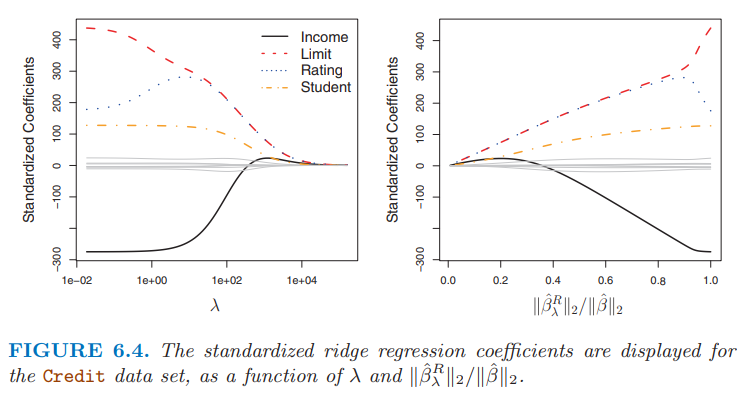
\includegraphics[scale=0.7]{images/ridge-reg.png}
\end{center}
At the extreme left-hand side of the plot, $\lambda$ is essentially zero, and so the corresponding ridge coefficient estimates are the same as the usual least squares estimates. But as $\lambda$ increases, the ridge coefficient estimates shrink towards zero. The right-hand panel of the Figure  displays the same ridge coefficient estimates as the left-hand panel, but instead of displaying $\lambda$ on the x-axis, we now display $||\hat{\beta}_\lambda^R||_2 / ||\hat{\beta}||_2$, where $\hat{\beta}$ denotes the vector of least squares coefficient estimates. The notation $||\hat{\beta}||_2$ denotes the $l_2$ norm of a vector, and is defined as $||\beta||_2 = \sqrt{\sum_{j=1}^p \beta_j^2}$. It measures the distance of $\beta$ from zero. As $\lambda$ increases, the $l_2$ norm of $\hat{\beta}_\lambda^R$ will always decreases, and so will $||\hat{\beta}_\lambda^R||_2 / ||\hat{\beta}||_2$.  The latter quantity ranges from 1 (when $\lambda = 0$) to 0 ((when $\lambda = \infty$). Therefore, we can think of the x-axis in the right-hand panel of the Figure as the amount that the ridge regression coefficient estimates have been shrunken towards zero.\\\\
The standard least squares coefficient estimates are scale invariant: multiplying $X_j$ by a constant $c$ simply leads to a scaling of the least squares coefficient estimates by a factor of $1/c$. In contrast, the ridge regression coefficient estimates can change substantially when multiplying a given predictor by a constant. Therefore, it is best to apply ridge regression after \textit{standardizing the predictors} so that they are all on the same scale.

\subsubsection{Why Does Ridge Regression Improve Over Least Squares?}
Ridge regression’s advantage over least squares is rooted in the bias-variance trade-off. As $\lambda$ increases, the flexibility of the ridge regression fit decreases, leading to decreased variance but increased bias. The green curve in the left-hand panel of the Figure below displays the variance of the ridge regression predictions as a function of $\lambda$.
\begin{center}
    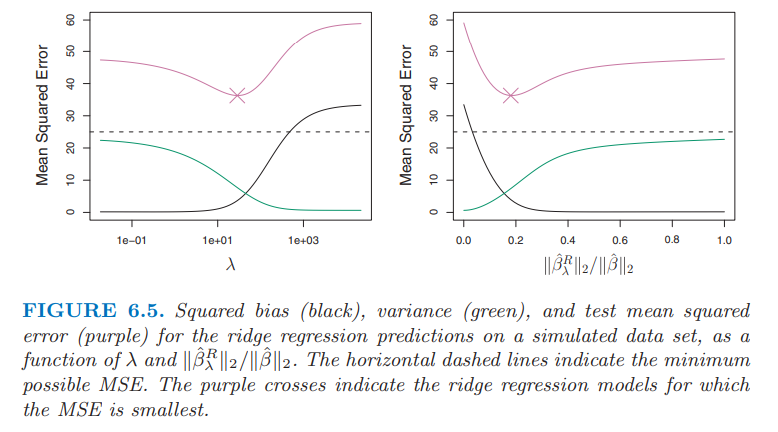
\includegraphics[scale=0.6]{images/ridge-reg-bias-variance.png}
\end{center}
At the least squares coefficient estimates, which correspond
to ridge regression with $\lambda = 0$, the variance is high but there is no bias. But as $\lambda$ increases, the shrinkage of the ridge coefficient estimates leads to a substantial reduction in the variance of the predictions, at the expense of a slight increase in bias. the MSE drops considerably as $\lambda$ increases from 0 to 10. Beyond this point, the decrease in variance due to increasing $\lambda$ slows, and the shrinkage on the coefficients causes them to be significantly underestimated, resulting in a large increase in the bias. The minimum MSE is achieved at approximately $\lambda = 30$.\\\\
Ridge regression works best in situations where the least squares estimates have high variance. Ridge regression also has substantial computational advantages over best subset selection, which requires searching through $2^p$ models. As we discussed previously, even for moderate values of $p$, such a search can be computationally infeasible. In contrast, for any fixed value of $\lambda$, ridge regression only fits a single model, and the model-fitting procedure can be performed quite quickly.

\subsection{The Lasso}
Ridge regression does have one obvious disadvantage. Unlike best subset, forward stepwise, and backward stepwise selection, which will generally select models that involve just a subset of the variables, ridge regression will include all $p$ predictors in the final model. The penalty term will shrink all of the coefficients towards zero, but it will not set any of them exactly to zero (unless $\lambda = \infty$). This may not be a problem for prediction accuracy, but it can create a challenge in model interpretation in settings in which the number of variables $p$ is quite large.\\\\
The lasso is a relatively recent alternative to ridge regression that overcomes this disadvantage. The lasso coefficients, $\hat{\beta}^L_\lambda$ , minimize the quantity
\begin{equation}
    RSS + \lambda \sum_{j=1}^p |\beta_j|
    \label{lasso}
\end{equation}
Comparing \ref{ridge-regression} to \ref{lasso}, we see that the lasso and ridge regression have similar formulations. The only difference is that the $\beta_j^2$ term in the ridge regression penalty has been replaced by $|\beta_j|$ in the lasso penalty. The lasso uses an $l_1$ penalty instead of a $l_2$ penalty. As with ridge regression, the lasso shrinks the coefficient estimates towards zero. However, in the case of the lasso, the $l_1$ penalty has the effect of forcing some of the coefficient estimates to be exactly equal to zero when the tuning parameter $\lambda$ is sufficiently large. Hence, much like best subset selection, the lasso performs \textit{variable selection}. As a result, models generated from the lasso are generally much easier to interpret than those produced by ridge regression. We say that the lasso yields \textit{sparse} models—that is, models that involve only a subset of the variables. 

\subsubsection{The Variable Selection Property of the Lasso}
Why is it that the lasso, unlike ridge regression, results in coefficient estimates that are exactly equal to zero? The figure below illustrates the situation. The least squares solution is marked as $\hat{\beta}$, while the blue diamond and circle represent the lasso and ridge regression constraints, respectively.
\begin{center}
    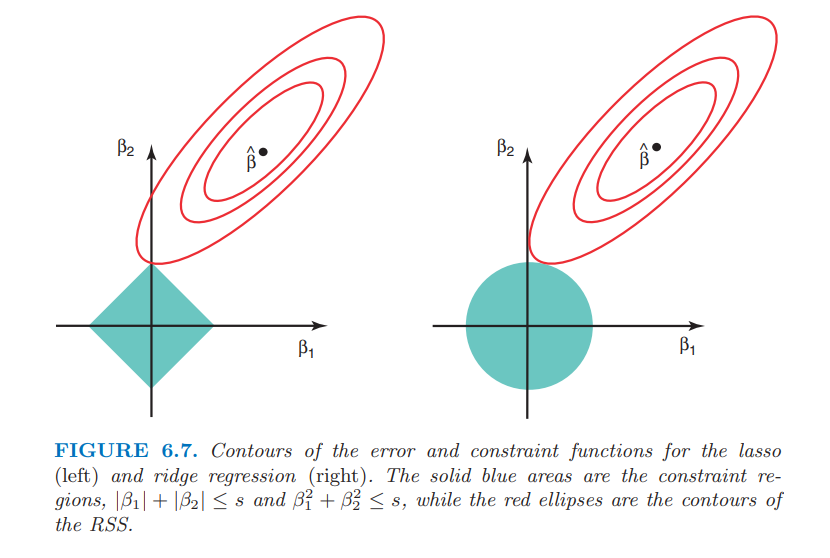
\includegraphics[scale=0.7]{images/ridge-lasso-geom.png}
\end{center}
The ellipses that are centered around $\hat{\beta}$ represent regions of constant
RSS. In other words, all of the points on a given ellipse share a common value of the RSS. As the ellipses expand away from the least squares coefficient estimates, the RSS increases. The lasso and ridge regression coefficient estimates are given by the first point at which an ellipse contacts the constraint region. Since ridge
regression has a circular constraint with no sharp points, this intersection will not generally occur on an axis, and so the ridge regression coefficient estimates will be exclusively non-zero. However, the lasso constraint has corners at each of the axes, and so the ellipse will often intersect the constraint region at an axis. When this occurs, one of the coefficients will equal zero. In higher dimensions, many of the coefficient estimates may equal zero simultaneously.

\subsection{Comparing the Lasso and Ridge Regression}
It is clear that the lasso has a major advantage over ridge regression, in that it produces simpler and more interpretable models that involve only a subset of the predictors. However, which method leads to better prediction accuracy? In general, one might expect the lasso to perform better in a setting where a relatively small number of predictors have substantial coefficients, and the remaining predictors have coefficients that are very small or that equal zero. Ridge regression will perform better when the response is a function of many predictors, all with coefficients of roughly equal size. A technique such as cross-validation can be used in order to determine which approach is better on a particular data set.

\subsection{Bayesian Interpretation for Ridge Regression and the Lasso}
We now show that one can view ridge regression and the lasso through
a Bayesian lens. A Bayesian viewpoint for regression assumes that the coefficient vector $\beta$ has some \textit{prior distribution}, say $p(\beta)$, where $\beta = (\beta_0, \beta_1,...,\beta_p)^T$. The likelihood of the data can be written as $f(Y |X, \beta)$, where $X = (X_1,...,X_p)$. Multiplying the prior distribution by the likelihood gives us (up to a proportionality constant) the \textit{posterior distribution}
\begin{equation}
    p(\beta| X, Y) \propto f(Y|X, \beta) p(\beta|X) = f(Y|X, \beta) p(\beta)
\end{equation}
where the proportionality above follows from Bayes’ theorem, and the equality above follows from the assumption that $X$ is fixed. We assume the usual linear model, and suppose that the errors are independent and drawn from a normal distribution. Furthermore, assume that $p(\beta) = \prod_{j=1}^p g(\beta_j)$, for some density
function $g$. It turns out that ridge regression and the lasso follow naturally
from two special cases of $g$:
\begin{itemize}
    \item  $g$ is a Gaussian distribution with mean zero and standard deviation a function of $\lambda$, then it follows that the posterior mode for $\beta$, that is, the most likely value for $\beta$, given the data, is given by the ridge regression solution.

    \item If $g$ is a double-exponential (Laplace) distribution with mean zero and scale parameter a function of $\lambda$, then it follows that the posterior mode for $\beta$ is the lasso solution.
\end{itemize}
Therefore, from a Bayesian viewpoint, ridge regression and the lasso follow directly from assuming the usual linear model with normal errors, together with a simple prior distribution for $\beta$.
\begin{center}
    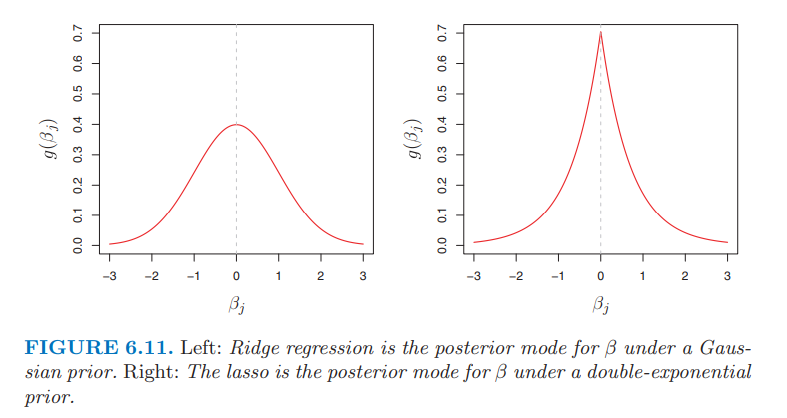
\includegraphics[scale=0.7]{images/ridge-lasso-bayesian.png}
\end{center}

Notice that the lasso prior is steeply peaked at zero, while the Gaussian is flatter and fatter at zero. Hence, the lasso expects a priori that many of the coefficients are (exactly) zero, while ridge assumes the coefficients are randomly distributed about zero.

\subsection{Selecting the Tuning Parameter}
Just as the subset selection approaches require a method to determine which of the models under consideration is best, implementing ridge regression and the lasso requires a method for selecting a value for the tuning parameter $\lambda$. Cross-validation provides a simple way to tackle this problem. We choose a grid of $\lambda$ values, and compute the cross-validation error for each value of $\lambda$. We then select the tuning parameter value for which the cross-validation error is smallest. Finally, the model is re-fit using all of the available observations and the selected value of the tuning parameter.

\section{High-Dimensional Data}
Most traditional statistical techniques for regression and classification are intended for the low-dimensional setting in which $n$, the number of observations, is much greater than $p$, the number of features. In the past 20 years, new technologies have changed the way that data are collected. While $p$ can be extremely large, the number of observations $n$ is often limited due to cost, sample availability, or other considerations.\\\\
Data sets containing more features than observations are often referred
to as \textit{high-dimensional}. Classical approaches such as least squares linear regression are not appropriate in this setting.

\subsection{What Goes Wrong in High Dimensions?}
When the number of features $p$ is as large as, or larger than, the number of observations $n$, least squares cannot (or rather,
should not) be performed. The reason is simple: regardless of whether or not there truly is a relationship between the features and the response, least squares will yield a set of coefficient estimates that result in a perfect fit to the data, such that the residuals are zero.\\\\
An example is shown in the Figure below with $p = 1$ feature (plus an intercept) in two cases: when there are 20 observations, and when there are only two observations.
\begin{center}
    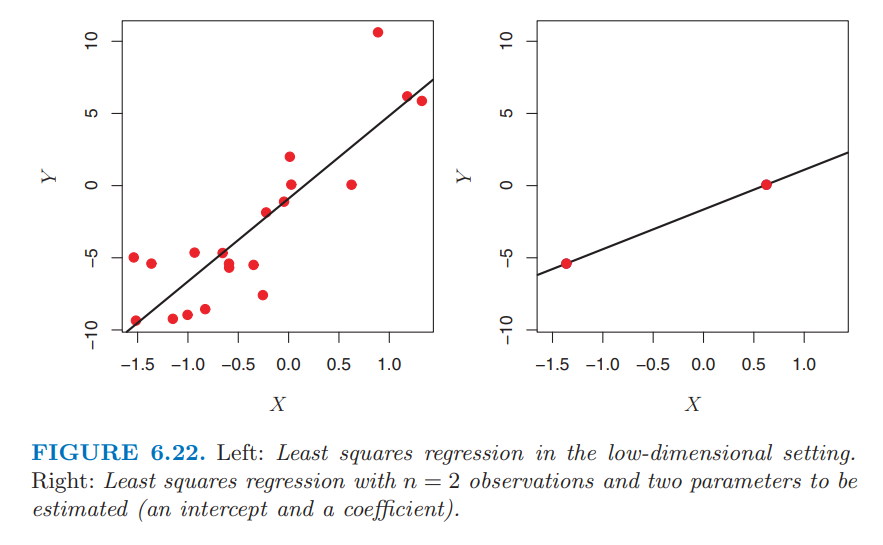
\includegraphics[scale=0.7]{images/high-dimensional.png}
\end{center}
When there are 20 observations, $n>p$, the least squares regression line does not perfectly fit the data. On the other hand, when there are only two observations, then regardless of the values of those observations, the regression line will fit the data exactly. This is problematic because this perfect fit will almost certainly lead to overfitting of the data. The problem is simple: when $p>n$ or $p \approx n$, a simple least squares regression line is too flexible and hence overfits the data.

\subsection{Regression in High Dimensions}
It turns out that many of the methods seen in this chapter for fitting
less flexible least squares models, such as forward stepwise selection, ridge regression, the lasso, and principal components regression, are particularly useful for performing regression in the high-dimensional setting. Essentially, these approaches avoid overfitting by using a less flexible fitting approach than least squares.\\\\
A key principle in the analysis of highdimensional data is the so called \textit{curse of dimensionality}. One might think that as the number of features used to fit a model increases, the quality of the fitted model will increase as well. However, this is not necessary the case. In general, adding additional signal features that are truly associated with the response will improve the fitted model, in the sense of leading to a reduction in test set error. However, adding
noise features that are not truly associated with the response will lead to a deterioration in the fitted model, and consequently an increased test set error. 

\chapter{Lec TBL-2 - Moving Beyond Linearity}

\section{Introduction}
So far, we have mostly focused on linear models. Linear models are relatively simple to describe and implement, and have advantages over other approaches in terms of interpretation and inference. However, standard linear regression can have significant limitations in terms of predictive power.  In this chapter we relax the linearity assumption while still attempting to maintain as much interpretability as possible. We do this by examining very simple extensions of linear models like polynomial regression and step functions, as well as more sophisticated approaches such as splines and generalized additive models.

\begin{itemize}
    \item \textit{Polynomial regression} extends the linear model by adding extra predictors, obtained by raising each of the original predictors to a power. For example, a cubic regression uses three variables, $X, X^2$, and $X^3$, as predictors.

    \item \textit{Step functions} cut the range of a variable into $K$ distinct regions in order to produce a qualitative variable. This has the effect of fitting a piecewise constant function.

    \item \textit{Regression splines} are more flexible than polynomials and step functions, and in fact are an extension of the two. They involve dividing the range of $X$ into $K$ distinct regions. Within each region, a polynomial function is fit to the data. However, these polynomials are constrained so that they join smoothly at the region boundaries, or knots.

    \item \textit{Smoothing splines} are similar to regression splines, but arise in a slightly different situation. Smoothing splines result from minimizing a residual sum of squares criterion subject to a smoothness penalty.

    \item \textit{Generalized additive models} allow us to extend the methods above to deal with multiple predictors.

\end{itemize}

\section{Polynomial Regression}
Historically, the standard way to extend linear regression to settings in which the relationship between the predictors and the response is nonlinear has been to replace the standard linear model with a polynomial function
\begin{equation}
    y_i = \beta_0 + \beta_1x_i + \beta_2x_i^2 + ... + \beta_dx_i^d + \epsilon_i
    \label{polynomial-reg}
\end{equation}
This approach is known as \textit{polynomial regression}. The coefficients in \ref{polynomial-reg} can be easily estimated using least squares linear regression because this is just a standard linear model with predictors $x_i, x_i^2, ..., x_i^d$. Generally speaking, it is unusual to use $d$ greater than 3 or 4 because for large values of $d$, the polynomial curve can become overly flexible and can take on some very strange shapes.

\section{Step Functions}
Using polynomial functions of the features as predictors in a linear model imposes a global structure on the non-linear function of $X$. We can instead use step functions in order to avoid imposing such a global structure. Here we break the range of $X$ into \textit{bins}, and fit a different constant in each bin. This amounts to converting a continuous variable into an \textit{ordered categorical variable}.\\\\
In greater detail, we create cutpoints $c_1, c_2,...,c_K$ in the range of $X$, and then construct $K + 1$ new variables
\[
\begin{split}
    C_0(X) & = I(X<c_1),\\
    C_1(X) & = I(c_1 \leq X < c_2),\\
    C_2(X) & = I(c_2 \leq X < c_3),\\
    & .\\
    & .\\
    & .\\
    C_{K-1}(X) & = I(c_{K-1} \leq X < c_K),\\
    C_K(X) & = I(c_K \leq X)
\end{split}
\]
These are sometimes called \textit{dummy variables}. Notice that for any value of $X$, $C_0(X) + C_1(X) + ... + C_K(X) = 1$, since $X$ must be in exactly one of the $K + 1$ intervals. We then use least squares to fit a linear model using $C_1(X), C_2(X),...,C_K(X)$ as predictors.
\begin{equation}
    y_i = \beta_0 + \beta_1C_1(x_i) + \beta_2C_2(x_i) + ... + \beta_KC_K(x_i) + \epsilon_i
    \label{step-function}
\end{equation}
Note that when $X<c_1$, all of the predictors in \ref{step-function} are zero, so $\beta_0$ can be interpreted as the mean value of $Y$ for $X<c_1$. By comparison, $\beta_j$ represents the average increase in the response for $X$ in $c_j \leq X < c_{j+1}$ relative to $X<c_1$.
\\\\
Unfortunately, unless there are natural breakpoints in the predictors, piecewise-constant functions can miss the action.  Nevertheless, step function approaches are very popular in biostatistics and epidemiology, among other disciplines. For example, 5-year age groups are often used to define the bins.

\section{Basis Functions}
Polynomial and piecewise-constant regression models are in fact special cases of a \textit{basis function} approach. The idea is to have at hand a family of functions or transformations that can be applied to a variable $X$: $b_1(X), b_2(X), ..., b_K(X)$. Instead of fitting a linear model in $X$, we fit the model
\begin{equation}
    y_i = \beta_0 + \beta_1b_1(x_i) + \beta_2b_2(x_i) + ... + \beta_Kb_K(x_i) + \epsilon_i
    \label{basis}
\end{equation}
For polynomial regression, the basis functions are $b_j(x_i) = x_i^j$ and for piecewise constant functions they are $b_j(X_i) = I(c_j \leq x_i < c_{j+1})$. We can think of \ref{basis} as a standard linear model with predictors $b_1(X), b_2(X), ..., b_K(X)$. Hence, we can use least squares to estimate the unknown regression coefficients in \ref{basis}.  Importantly, this means that all of the inference tools for linear models are available in this setting.\\\\
Thus far we have considered the use of polynomial functions and piecewise constant functions for our basis functions; however, many alternatives are possible. For instance, we can use wavelets or Fourier series to construct basis functions. In the next section, we investigate a very common choice for a basis function: \textit{regression splines}.

\section{Regression Splines}
Now we discuss a flexible class of basis functions that extends upon the polynomial regression and piecewise constant regression approaches that we have just seen.

\subsection{Piecewise Polynomials}
Instead of fitting a high-degree polynomial over the entire range of $X$, \textit{piecewise polynomial regression} involves fitting separate low-degree polynomials over different regions of $X$. For example, a piecewise cubic polynomial works by fitting a cubic regression model of the form
\begin{equation}
     y_i = \beta_0 + \beta_1x_i + \beta_2x_i^2 + \beta_3x_i^3 + \epsilon_i
     \label{cubic-pol}
\end{equation}
where the coefficients $\beta_0, \beta_1, \beta_2$, and $\beta_3$ differ in different parts of the range of $X$. The points where the coefficients change are called \textit{knots}.A piecewise cubic polynomial with a single knot at a point $c$ takes the form
\[
y_i =
\begin{cases}
     \beta_{01} + \beta_{11}x_i + \beta_{21}x_i^2 + \beta_{31}x_i^3 + \epsilon_i & \text{if } x_i < c;\\
\beta_{02} + \beta_{12}x_i + \beta_{22}x_i^2 + \beta_{32}x_i^3 + \epsilon_i & \text{if } x_i \geq c.   
\end{cases}
\]
Each of these polynomial functions can be fit using least squares applied to simple functions of the original predictor (more details later). If we place $K$ different knots throughout the range of $X$, then we will end up fitting $K + 1$ different cubic polynomials. Note that we do not need to use a cubic polynomial. For example, we can instead fit piecewise linear functions. In fact, our piecewise constant functions defined previously are piecewise polynomials of degree 0. A piecewise cubic polynomial (4 parameters) fitted with a single knot uses a total of $4 \times 2 = 8$ \textit{degrees of freedom}. Basically, the degrees of freedom are the number of parameters to be estimated.

\subsection{Constraints and Splines}
The top left panel of the Figure below shows a piecewise cubic polynomial fit to
a subset of the Wage data, with a single knot at $age=50$. 
\begin{center}
    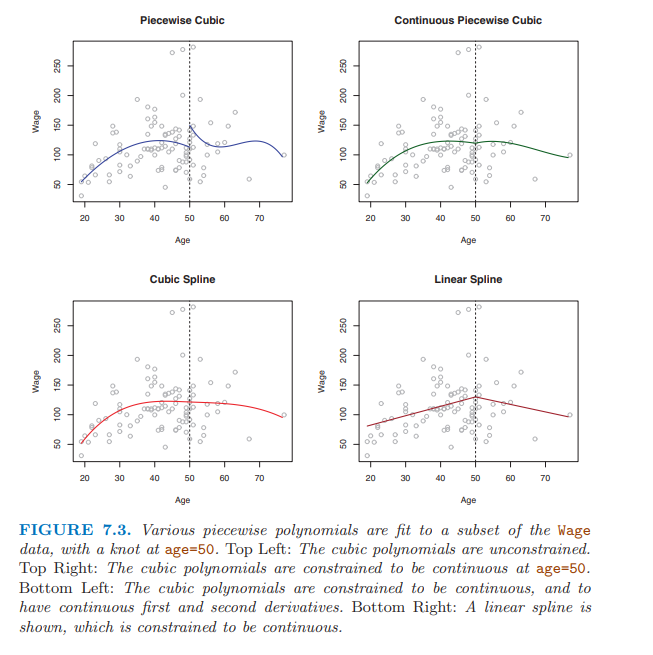
\includegraphics[scale=0.6]{images/B-spline.png}
\end{center}
It  looks wrong because the fitted curve is just too flexible. To remedy this problem, we can fit a piecewise polynomial under the constraint that the fitted curve must be continuous. The top right plot in the Figure shows the resulting fit. This looks better than the top left plot, but the V-shaped join looks unnatural.\\\\
In the lower left plot, we have added two additional constraints: now both
the first and second derivatives of the piecewise polynomials are continuous at $age=50$. In other words, we are requiring that the piecewise polynomial
be not only continuous when $age=50$, but also very \textit{smooth}. So in the top left plot, we are using eight degrees of freedom, but in the bottom left plot we imposed three constraints (continuity, continuity of the first derivative, and continuity of the second derivative) and so are left with five degrees of freedom. The curve in the bottom left plot is called a \textit{cubic spline}. In general, a cubic spline with $K$ knots uses a total of $4 + K$ degrees of freedom.\\\\
The general definition of a degree-$d$ spline is that it is a piecewise degree-$d$ polynomial, with continuity in derivatives up to degree $d - 1$ at each knot. In order to determine the degrees of freedom of a degree-$d$ spline with $K$ knots, we can use the following formula:
\[(d+1)(K+1) - dK\]

\subsection{The Spline Basis Representation}
How can we fit a piecewise degree-$d$ polynomial under the constraint that it (and possibly its first $d - 1$ derivatives) be continuous? It turns out that we can use the basis model \ref{basis} to represent a regression spline. A cubic spline with $K$ knots can be modeled as
\begin{equation}
    y_i = \beta_0 + \beta_1b_1(x_i) + \beta_2b_2(x_i) + ... + \beta_{K+3}b_{K+3}(x_i) + \epsilon_i
    \label{reg-spline}
\end{equation}
for an appropriate choice of basis functions $b_1, b_2,...,b_{K+3}$. The model \ref{reg-spline} can then be fit using least squares.\\\\
The most direct way to represent a cubic spline using \ref{reg-spline} is to start off with a basis for a cubic polynomial, namely, $x, x^2, x^3$, and then add one \textit{truncated power basis} function per knot. A truncated power basis function is defined as 
\begin{equation}
    h(x, \xi) = (x - \xi)^3_+ = 
    \begin{cases}
        (x - \xi)^3 & \text{if } x > \xi\\
        0 & \text{otherwise}
    \end{cases}
\end{equation}
where $\xi$ is the knot. One can show that adding a term of the form $\beta_4h(x, \xi)$ to the model \ref{cubic-pol} for a cubic polynomial will lead to a discontinuity in only the third derivative at $\xi$; the function will remain continuous, with continuous first and second derivatives, at each of the knots.\\\\
In other words, in order to fit a cubic spline to a data set with $K$ knots, we
perform least squares regression with an intercept and $3 + K$ predictors, of the form $X, X^2, X^3, h(X, \xi_1), h(X, \xi_2), ..., h(X, \xi_K)$, where $\xi_1, \xi_2, ..., \xi_K$ are the knots. This amounts to estimating a total of $K + 4$ regression coefficients;  for this reason, fitting a cubic spline with $K$ knots uses $K+4$ degrees of freedom. In general, for a degree-$d$ spline we need $d$ parameters plus one parameter per knot and the intercept.\\\\
Unfortunately, splines can have high variance at the outer range of the predictors, that is, when $X$ takes on either a very small or very large value. A \textit{natural spline} is a regression spline with additional \textit{boundary constraints}: the function is required to be linear at the boundary. This additional constraint means that natural splines are less flexible than regression splines (a natural spline with $K$ knots has $K$ degrees of freedom), and generally produces more stable estimates at the boundaries.

\subsection{Choosing the Number and Locations of the Knots}
When we fit a spline, where should we place the knots? The regression spline is most flexible in regions that contain a lot of knots, because in those regions the polynomial coefficients can change rapidly. Hence, one option is to place more knots in places where we feel the function might vary most rapidly, and to place fewer knots where it seems more stable. While this option can work well, in practice it is common to place knots in a uniform fashion. One way to do this is to specify the desired degrees of freedom, and then have the software automatically place the corresponding number of knots at uniform quantiles of the data.\\\\
How many knots should we use, or equivalently how many degrees of freedom should our spline contain? One option is to try out different numbers of knots and see which produces the best looking curve. A somewhat more objective approach is to use cross-validation.

\subsection{Comparison to Polynomial Regression}
Regression splines often give superior results to polynomial regression. This
is because unlike polynomials, which must use a high degree (exponent in
the highest monomial term, e.g. $X^{15}$) to produce flexible fits, splines introduce flexibility by increasing the number of knots but keeping the degree
fixed. Then, a degree-15 polynomial function will assume very strange shapes more likely to overfit the data. Instead, a regression spline with the same flexibility (in terms of numbers of parameters) can be obtained with a cubic spline with 12 knots, which will produce a smoother fit less sensible to overfitting.

\section{Smoothing Splines}
\subsection{ An Overview of Smoothing Splines}
In the last section we discussed regression splines, which we create by specifying a set of knots, producing a sequence of basis functions, and then using least squares to estimate the spline coefficients. We now introduce a somewhat different approach that also produces a spline.\\\\
In fitting a smooth curve to a set of data, what we really want to do is find some function, say $g(x)$, that fits the observed data well: that is, we want RSS to be small. However, there is a problem with this approach. If we don’t put any constraints on $g(x_i)$, then we can always make RSS zero simply by choosing $g$ such that it interpolates all of the $y_i$, leading to overfitting. What we really want is a function g that makes RSS small, but that is also smooth.\\\\
How might we ensure that $g$ is smooth? There are a number of ways to do this. A natural approach is to find the function $g$ that minimizes
\begin{equation}
    \sum_{i=1}^n (y_i - g(x_i))^2 + \lambda \int g''(t)^2 dt
    \label{smoothing-spline}
\end{equation}
where $\lambda$ is a nonnegative tuning parameter. The function g that minimizes \ref{smoothing-spline} is known as a \textit{smoothing spline}. Equation \ref{smoothing-spline}  takes the “Loss+Penalty” formulation that we encounter in the context of ridge regression and the lasso. The first term is a \textit{loss function} that encourages $g$ to fit the data well, while the second term is a \textit{penalty term} hat penalizes the variability in $g$. The notation $g''(t)$ indicates the second derivative of the function $g$. The first derivative $g'(t)$
measures the slope of a function at $t$, and the second derivative corresponds to the amount by which the slope is changing. Hence, the second derivative is large in absolute value if $g(t)$ is very wiggly near $t$, and it is close to zero otherwise. The integral simply measures the total change in the function $g'(t)$, over its entire range. If $g$ is very smooth, then $g'(t)$ will be close to constant and $\int g''(t)^2 dt$ will take on a small value. Conversely, if $g$ is jumpy and variable, $\int g''(t)^2 dt$ will take on large values.\\\\
The larger the value of $\lambda$, the smoother $g$ will be. When $\lambda \rightarrow \infty$, $g$ will be perfectly smooth—it will just be a straight line that passes as closely as possible to the training points. In fact, in this case, $g$ will be the linear least squares line.\\\\
The function $g(x)$ that minimizes \ref{smoothing-spline}  can be shown to have some special properties: it is a piecewise cubic polynomial with knots at the unique
values of $x_1,...,x_n$, and continuous first and second derivatives at each knot. Furthermore, it is linear in the region outside of the extreme knots. In other words, the function $g(x)$ that minimizes \ref{smoothing-spline} is a natural cubic
spline with knots at $x_1,...,x_n$. However, it is not the same natural cubic
spline that one would get if one applied the basis function approach described previously with knots at $x_1,...,x_n$. Rather, it is a \textit{shrunken} version of such a natural cubic spline, where the value of the tuning parameter $\lambda$ controls the level of shrinkage.

\subsection{Choosing the Smoothing Parameter $\lambda$}
We have seen that a smoothing spline is simply a natural cubic spline with knots at every unique value of $x_i$. It might seem that a smoothing spline will have far too many degrees of freedom, since a knot at each data point allows a great deal of flexibility. But the tuning parameter $\lambda$ controls the roughness of the smoothing spline, and hence the \textit{effective degrees of freedom}.\\\\
In the context of smoothing splines, why do we discuss effective degrees of freedom instead of degrees of freedom? Usually degrees of freedom refer to the number of free parameters, such as the number of coefficients fit in a polynomial or cubic spline. Although a smoothing spline has $n$ parameters and hence $n$ nominal degrees of freedom, these $n$ parameters are heavily constrained or shrunk down. Hence $df_\lambda$ is a measure of the flexibility of the smoothing spline, the higher it is, the more flexible the smoothing spline.\\\\
In fitting a smoothing spline, we do not need to select the number or location of the knots. Instead, we have another problem: we need to choose the value of $\lambda$. It should come as no surprise that one possible solution to this problem
is cross-validation. It turns out that the \textit{leaveone-out} cross-validation error (LOOCV) can be computed very efficiently for smoothing splines.

\section{Generalized Additive Models}
In the previous sections we present a number of approaches for flexibly predicting a response $Y$ on the basis of a single predictor $X$. Here we explore the problem of flexibly predicting $Y$ on the basis of several predictors, $X_1,...,X_p$.\\\\
Generalized additive models (GAMs) provide a general framework for extending a standard linear model by allowing non-linear functions of each of the variables, while maintaining \textit{additivity}.

\subsection{GAMs for Regression Problems}
A natural way to extend the multiple linear regression model in order to allow for non-linear relationships between each feature and the response is to replace each linear component $\beta_jx_{ij}$ with a (smooth) nonlinear function $f_j(x_{ij})$. We would then write the model as
\begin{equation}
    y_i = \beta_0 + \sum_{j=1}^p f_j(x_{ij}) + \epsilon_i
\end{equation}
In the previous sections, we discussed many methods for fitting functions to a single variable. The beauty of GAMs is that we can use these methods as building blocks for fitting an additive model.\\\\
Fitting a GAM with a smoothing spline is not quite as simple as fitting a GAM with a natural spline, since in the case of smoothing splines, least squares cannot be used. However, standard software can be used to fit GAMs using smoothing splines, via an approach known as backfitting.

\subsection{Pros and Cons of GAMs}
Let us summarize the advantages and limitations of a GAM.\\\\
\textbf{Pros:}
\begin{itemize}
    \item GAMs allow us to fit a non-linear $f_j$ to each $X_j$ , so that we can automatically model non-linear relationships that standard linear regression will miss.

    \item The non-linear fits can potentially make more accurate predictions for the response $Y$.

    
    \item Because the model is additive, we can still examine the effect of each $X_j$ on $Y$ individually while holding all of the other variables fixed.

    \item The smoothness of the function $f_j$ for the variable $X_j$ can be summarized via degrees of freedom.
\end{itemize}
\textbf{Cons:}
\begin{itemize}
    \item The main limitation of GAMs is that the model is restricted to be additive. With many variables, important interactions can be missed. However, as with linear regression, we can manually add interaction terms to the GAM model by including additional predictors of the form $X_j \times X_k$.
\end{itemize}


\chapter{Lec 20-21-22 - Tree-Based Methods}

\section{Introduction}
In this chapter, we describe tree-based methods for regression and classification. These involve stratifying or segmenting the predictor space into a number of simple regions. In order to make a prediction for a given observation, we typically use the mean or the mode of the training observations in the region to which it belongs.\\\\
Tree-based methods are simple and useful for interpretation. However,
they typically are not competitive with the best supervised learning approaches in terms of prediction accuracy. Hence in this chapter we also introduce \textit{bagging} and \textit{random forests}. Each of these approaches involves producing multiple trees which are then combined to yield a single consensus prediction.

\section{The Basics of Decision Trees}
Decision trees can be applied to both regression and classification problems.
We first consider regression problems, and then move on to classification.

\subsection{Regression Trees}
In order to motivate regression trees, we begin with a simple example.

\subsubsection{Predicting Baseball Players’ Salaries Using Regression Trees}
We use the Hitters data set to predict a baseball player’s \textit{Salary} based on \textit{Years} (the number of years that he has played in the major leagues) and \textit{Hits} (the number of hits that he made in the previous year). We first remove observations that are missing \textit{Salary} values, and log-transform \textit{Salary} so that its distribution has more of a typical bell-shape. The Figure below  shows a regression tree fit to this data. It consists of a series of splitting rules, starting at the top of the tree. The top split assigns observations having $Years<4.5$ to the left branch.
\begin{center}
    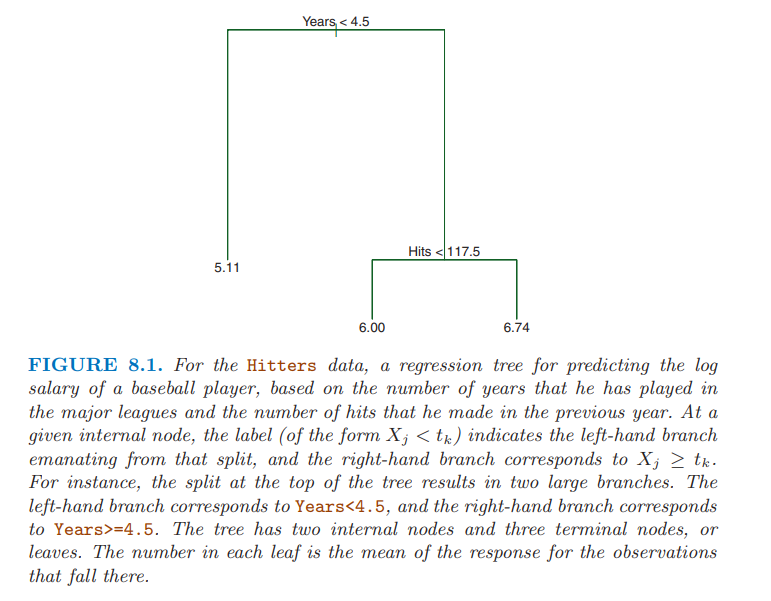
\includegraphics[scale=0.7]{images/reg-tree.png}
\end{center}
The predicted salary for these players is given by the mean response value for the players in the data set with $Years<4.5$. Overall, the tree stratifies
or segments the players into three regions of predictor space: players who have played for four or fewer years, players who have played for five or more years and who made fewer than 118 hits last year, and players who have played for five or more years and who made at least 118 hits last year. The figure below  illustrates the regions as a function of \textit{Years} and \textit{Hits}
\begin{center}
    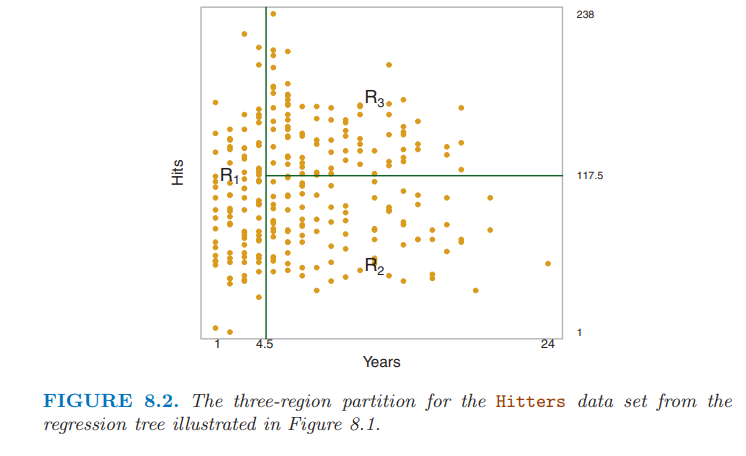
\includegraphics[scale=0.7]{images/reg-tree-2.png}
\end{center}
We might interpret this regression tree as follows: \textit{Years} is the most important factor in determining \textit{Salary}, and players with less experience earn lower salaries than more experienced players. Given that a player is less experienced, the number of hits that he made in the previous year seems to play little role in his salary. But among players who have been in the major leagues for five or more years, the number of hits made in the previous year does affect salary, and players who made more hits last year tend to have higher salaries.

\subsubsection{Prediction via Stratification of the Feature Space}
We now discuss the process of building a regression tree. Roughly speaking,
there are two steps.
\begin{enumerate}
    \item  We divide the predictor space, that is, the set of possible values for $X_1, X_2,...,X_p$, into $J$ distinct and non-overlapping regions, $R_1, R_2,...,R_J$.

    \item For every observation that falls into the region $R_j$ , we make the same prediction, which is simply the mean of the response values for the training observations in $R_j$.
\end{enumerate}
How do we construct the regions $R_1,...,R_J$? In theory, the regions could have any shape. However, we choose to divide the predictor space into high-dimensional rectangles, or boxes, for simplicity and for ease of interpretation of the resulting predictive model. The goal is to find boxes $R_1,...,R_J$ that minimize the RSS, given by
\begin{equation}
    \sum_{j=1}^J\sum_{i \in R_j}(y_i - \hat{y}_{R_j})^2
\end{equation}
where $\hat{y}_{R_j}$ is the mean response for the training observations within the $j$th box. Unfortunately, it is computationally infeasible to consider every
possible partition of the feature space into $J$ boxes. For this reason, we take
a \textit{top-down}, \textit{greedy} approach that is known as \textit{recursive binary splitting}. The approach is top-down because it begins at the top of the tree  and then successively splits the predictor space; each split is indicated via two new branches further down on the tree. It is greedy because at each step of the tree-building process, the best split is made at that particular step, rather than looking ahead and picking a split that will lead to a better tree in some future step.\\\\
In order to perform recursive binary splitting, we first select the predictor $X_j$ and the cutpoint $s$ such that splitting the predictor space into the regions $\{X|X_j < s\}$ and $\{X|X_j \geq s\}$ leads to the greatest possible
reduction in RSS. In greater detail, for any $j$ and $s$, we define the pair of half-planes
\[R_1(j,s) = \{X|X_j < s\} \quad \text{and} \quad R_2(j, s) = \{X|X_j \geq s\}\]
and we seek the value of j and s that minimize the equation
\begin{equation}
    \sum_{i:x_i \in R_1(j, s)}(y_i - \hat{y}_{R_1})^2 + \sum_{i:x_i \in R_2(j, s)}(y_i - \hat{y}_{R_2})^2
    \label{rec-split}
\end{equation}
Finding the values of j and s that minimize \ref{rec-split} can be done quite quickly, especially when the number of features $p$ is not too large. Next, we repeat the process, looking for the best predictor and best cutpoint in order to split the data further so as to minimize the RSS within each of the resulting regions. However, this time, instead of splitting the entire predictor space, we split one of the two previously identified regions. We now have three regions. Again, we look to split one of these three regions further, so as to minimize the RSS. The process continues until a stopping criterion is reached; for instance, we may continue until no region contains more than five observations.

\subsubsection{Tree Pruning}
The process described above may produce good predictions on the training set, but is likely to overfit the data. This is because the resulting tree might be too complex. A smaller tree with fewer splits might lead to lower variance and better interpretation at the cost of a little bias. One possible alternative to the process described above is to build the tree only so long as the decrease in the RSS due to each split exceeds some (high) threshold. This strategy will result in smaller trees, but is too short-sighted since a seemingly worthless split early on in the tree might be followed by a very good split. Therefore, a better strategy is to grow a very large tree $T_0$, and then \textit{prune} it back in order to obtain a subtree. Intuitively, our goal is to select a subtree that leads to the lowest test error rate. Given a subtree, we can estimate its test error using cross-validation or the validation set approach. However, estimating the cross-validation error for every possible subtree would be too cumbersome, since there is an extremely large number of possible subtrees. Instead, we need a way to select a small set of subtrees for consideration.\\\\
\textit{Cost complexity pruning} gives us a way to do just this. Rather than considering every possible subtree, we consider a sequence of trees indexed by a nonnegative tuning parameter $\alpha$. For each value of $\alpha$ there corresponds a subtree $T \subset T_0$ such that
\begin{equation}
    \sum_{m=1}^{|T|}\sum_{i:x_i \in R_m}(y_i - \hat{y}_{R_m})^2 + \alpha|T|
    \label{pruning}
\end{equation}
is minimized. Here $|T|$ indicates the number of terminal nodes of the tree $T$. The tuning parameter $\alpha$ controls a trade-off between the subtree’s complexity and its fit to the training data. Equation \ref{pruning} is reminiscent of the lasso, in which a similar formulation was used in order to control the complexity of a linear model.\\\\
It turns out that as we increase $\alpha$ from zero in \ref{pruning}, branches get pruned from the tree in a nested and predictable fashion, so obtaining the whole sequence of subtrees as a function of $\alpha$ is easy. We can select a value of $\alpha$ using a validation set or using cross-validation. This process is summarized in the Algorithm below.
\begin{center}
    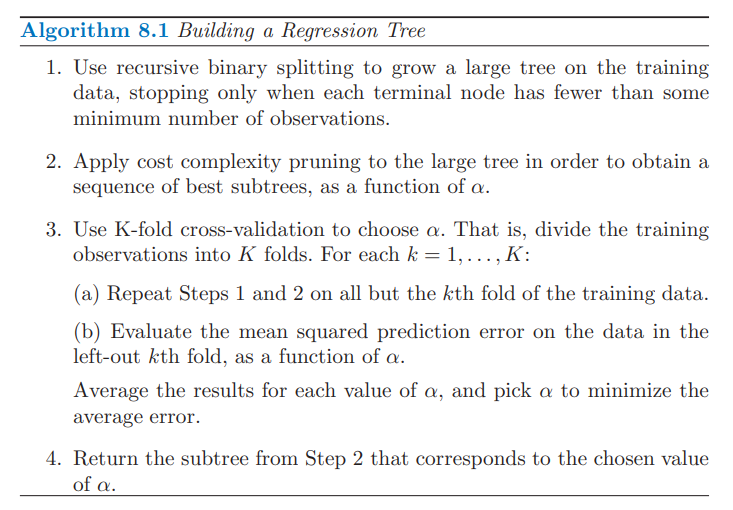
\includegraphics[scale=0.7]{images/pruning.png}
\end{center}

\subsection{Classification Trees}
A \textit{classification tree} is very similar to a regression tree, except that it is used to predict a qualitative response rather than a quantitative one. Recall that  for a regression tree, the predicted response for an observation is given by the mean response of the training observations that belong to the same terminal node. In contrast, for a classification tree, we predict that each observation belongs to the most commonly occurring class of training observations in the region to which it belongs.\\\\
In the classification setting, RSS cannot be used as a criterion for making the binary splits. A natural alternative to RSS is the \textit{classification error rate}, which is simply the fraction of the training observations in that region that do not belong to the most common class:
\begin{equation}
    E = 1 - max_k(\hat{p}_{mk})
\end{equation}
Here $\hat{p}_{mk}$ represents the proportion of training observations in the $m$th region that are from the $k$th class. However, it turns out that classification error is not sufficiently sensitive for tree-growing, and in practice two other measures are preferable.
\\\\
The \textit{Gini index} is defined by
\begin{equation}
    G = \sum_{k=1}^K \hat{p}_{mk}(1 - \hat{p}_{mk})
\end{equation}
a measure of total variance across the $K$ classes. It is not hard to see
that the Gini index takes on a small value if all of the $\hat{p}_{mk}$’s are close to zero or one. For this reason the Gini index is referred to as a measure of \textit{node purity}, a small value indicates that a node contains predominantly observations from a single class.\\\\
An alternative to the Gini index is cross-entropy, given by
\begin{equation}
    D = -\sum_{k=1}^K \hat{p}_{mk} log\, (\hat{p}_{mk})
\end{equation}
One can show that the cross-entropy will take on a value near zero if the $\hat{p}_{mk}$’s are all near zero or near one. Therefore, like the Gini index, the cross-entropy will take on a small value if the $m$th node is pure.\\\\
When building a classification tree, either the Gini index or the cross-entropy are typically used to evaluate the quality of a particular split. Any of these three approaches might be used when pruning the tree, but the classification error rate is preferable if prediction accuracy of the final pruned tree is the goal.\\\\
In our discussion thus far, we have assumed that the predictor variables take on continuous values. However, decision trees can be constructed even in the presence of qualitative predictor variables.\\\\
The figure below has a surprising characteristic: some of the splits yield two terminal nodes that have the same predicted value.
\begin{center}
    \includegraphics[scale=0.8]{images/classification-tree.png}
\end{center}
For instance, consider the split $RestECG<1$ near the bottom right of the unpruned tree. Regardless of the value of \textit{RestECG}, a response value of \textit{Yes} is predicted for those observations. Why, then, is the split performed at all? The split is performed because it leads to increased \textit{node purity}. That is, all 9 of the observations corresponding to the right-hand leaf have a response value of \textit{Yes}, whereas 7/11 of those corresponding to the left-hand leaf have a response value of \textit{Yes}. Why is node purity important? Suppose that we have a test observation that belongs to the region given by that right-hand leaf. Then we can be pretty certain that its response value is \textit{Yes}. In contrast, if a test observation belongs to the region given by the left-hand leaf, then its response value is probably \textit{Yes}, but we are much less certain. Even though the split \textit{RestECG<1} does not reduce the classification error, it improves the Gini index and the cross-entropy, which are more sensitive to node purity.

\subsection{Trees Versus Linear Models}
Regression and classification trees have a very different flavor from the more
classical approaches for regression and classification presented in the previous Chapters, such as linear regression. Which model is better? It depends on the problem at hand. If the relationship between the features and the response is well approximated by a linear model, then an approach such as linear regression
will likely work well, and will outperform a method such as a regression tree that does not exploit this linear structure. If instead there is a highly
non-linear and complex relationship between the features and the response, then decision trees may outperform classical approaches. Furthermore, in certain settings, prediction using a tree may be preferred for the sake of interpretability and visualization.
\begin{center}
    \includegraphics[scale=.7]{images/lin-reg-vs-reg-tree.png}
\end{center}

\subsection{Advantages and Disadvantages of Trees}
Decision trees for regression and classification have a number of advantages
over the more classical approaches:\\\\
\textbf{Pros:}
\begin{itemize}
    \item Trees are very easy to explain to people.
    
    \item Some people believe that decision trees more closely mirror human decision-making than do the regression and classification approaches.

    \item Trees can be displayed graphically.

    \item Trees can easily handle qualitative predictors without the need to create dummy variables. 
\end{itemize}
\textbf{Cons:}
\begin{itemize}
    \item Unfortunately, trees generally do not have the same level of predictive accuracy as some of the other regression and classification approaches.
\end{itemize}
However, by aggregating many decision trees, using methods like \textit{bagging} and \textit{random forests}, the predictive performance of trees can be
substantially improved.

\section{Bagging and Random Forests}
\subsection{Bagging}
The decision trees discussed previously suffer from high variance. This means that if we split the training data into two parts at random, and fit a decision tree to both halves, the results that we get could be quite different. In contrast, a procedure with low variance will yield similar results if applied repeatedly to distinct data sets. \textit{Bootstrap aggregation}, or \textit{bagging}, is a general-purpose procedure for reducing the variance of a statistical learning method; we introduce it here because it is particularly useful and frequently used in the context of decision trees.\\\\
Recall that given a set of $n$ independent observations $Z_1,...,Z_n$, each
with variance $\sigma^2$, the variance of the mean $\Bar{Z}$ of the observations is given by $\sigma^2/n$. In other words, averaging a set of observations reduces variance. Hence a natural way to reduce the variance and hence increase the prediction accuracy of a statistical learning method is to take many training sets from the population, build a separate prediction model using each training set, and average the resulting predictions. Of course, this is not practical because we generally do not have access to multiple training sets. Instead, we can \textit{bootstrap}, by taking repeated samples from the (single) training data set. In this approach we generate $B$ different bootstrapped training data sets. We then train our method on the $b$th bootstrapped training set, and finally average all the predictions. 
\\\\
While bagging can improve predictions for many regression methods, it is particularly useful for decision trees. Each of the $B$ trees is grown deep (on the $b$th bootstrapped training set), and are not pruned. Hence each individual tree has high variance, but low bias. Averaging these $B$ trees reduces the variance. How can bagging be extended to a classification problem where $Y$ is qualitative? In that situation, there are a few possible approaches, but the simplest is as follows. For a given test observation, we can record the class predicted by each of the B trees, and take a \textit{majority vote}: the overall prediction is the most commonly occurring class among the $B$ predictions.

\subsubsection{Out-of-Bag Error Estimation}
It turns out that there is a very straightforward way to estimate the test error of a bagged model, without the need to perform cross-validation or the validation set approach. One can show that on average, each bagged tree makes use of around two-thirds of the observations. The remaining one-third of the observations not used to fit a given bagged tree are referred to as the out-of-bag (OOB) observations. We can predict the response for the $i$th observation using each of the trees in which that observation was OOB. This will yield around $B/3$ predictions for the $i$th observation. In order to obtain a single prediction for the $i$th observation, we can average these predicted responses (or can take a majority vote). This leads to a single OOB prediction for the $i$th observation. An OOB prediction can be obtained in this way for each of the $n$ observations, from which the overall OOB MSE or classification error can be computed. The resulting OOB error is a valid estimate of the test error for the bagged model, since the response for each observation is predicted using only the trees that were not fit using that observation.

\subsubsection{Variable Importance Measures}
As we have discussed, bagging typically results in improved accuracy over
prediction using a single tree. Unfortunately, however, it can be difficult to
interpret the resulting model. When we bag a large number of trees, it is no longer possible to represent the resulting statistical learning procedure using a single tree. Thus, bagging improves prediction accuracy at the expense of interpretability.\\\\
Although the collection of bagged trees is much more difficult to interpret
than a single tree, one can obtain an overall summary of the importance of
each predictor using the RSS (or the Gini index). In the case of bagging regression trees, we can record the total amount that the RSS  is decreased due to splits over a given predictor, averaged over all $B$ trees. A large value indicates an important predictor.

\subsection{Random Forests}
Random forests provide an improvement over bagged trees by way of a small tweak that \textit{decorrelates} the trees. As in bagging, we build a number of decision trees on bootstrapped training samples. But when building these decision trees, each time a split in a tree is considered, a random sample of $m$ predictors is chosen as split candidates from the full set of $p$ predictors. The split is allowed to use only one of those $m$ predictors. Typically we choose $m \approx \sqrt{p}$.\\\\
In other words, in building a random forest, at each split in the tree,
the algorithm is not even allowed to consider a majority of the available
predictors. This may sound crazy, but it has a clever rationale. Suppose that there is one very strong predictor in the data set, along with a number of other moderately strong predictors. Then in the collection of bagged trees, most or all of the trees will use this strong predictor in the top split. Consequently, all of the bagged trees will look quite similar to each other. Hence the predictions from the bagged trees will be highly correlated. Unfortunately,  averaging many highly correlated quantities does not lead to as large of a reduction in variance as averaging many uncorrelated quantities.\\\\
Random forests overcome this problem by forcing each split to consider only a subset of the predictors. Therefore, on average $(p - m)/p$ of the splits will not even consider the strong predictor, and so other predictors will have more of a chance. Using a small value of $m$ in building a random forest will typically be helpful when we have a large number of correlated predictors.


\end{document}
